%%%%%%%%%%%%%%%%%%%%%%%%%%%%%%%%%%%%%%%%%
% Masters/Doctoral Thesis 
% LaTeX Template
% Version 2.3 (25/3/16)
%
% This template has been downloaded from:
% http://www.LaTeXTemplates.com
%
% Version 2.x major modifications by:
% Vel (vel@latextemplates.com)
%
% This template is based on a template by:
% Steve Gunn (http://users.ecs.soton.ac.uk/srg/softwaretools/document/templates/)
% Sunil Patel (http://www.sunilpatel.co.uk/thesis-template/)
%
% Template license:
% CC BY-NC-SA 3.0 (http://creativecommons.org/licenses/by-nc-sa/3.0/)
%
%%%%%%%%%%%%%%%%%%%%%%%%%%%%%%%%%%%%%%%%%

%% Note: To include the bibliography -> run pdflatex main.tex > bibtex main.aux > pdflatex main.tex > pdflatex main.tex

%----------------------------------------------------------------------------------------
%	PACKAGES AND OTHER DOCUMENT CONFIGURATIONS
%----------------------------------------------------------------------------------------

\documentclass[
  12pt, % The default document font size, options: 10pt, 11pt, 12pt
  %oneside, % Two side (alternating margins) for binding by default, uncomment to switch to one side
  %chapterinoneline,% Have the chapter title next to the number in one single line
  english, % ngerman for German
  doublespacing, % Single line spacing, alternatives: singlespacing, onehalfspacing or doublespacing
  %draft, % Uncomment to enable draft mode (no pictures, no links, overfull hboxes indicated)
  %nolistspacing, % If the document is onehalfspacing or doublespacing, uncomment this to set spacing in lists to single
  %liststotoc, % Uncomment to add the list of figures/tables/etc to the table of contents
  %toctotoc, % Uncomment to add the main table of contents to the table of contents
  %parskip, % Uncomment to add space between paragraphs
  %nohyperref, % Uncomment to not load the hyperref package
  %headsepline, % Uncomment to get a line under the header
]{setting} % The class file specifying the document structure

\usepackage[utf8]{inputenc} % Required for inputting international characters
\usepackage[T1]{fontenc} % Output font encoding for international characters
\usepackage{palatino} % Use the Palatino font by default
\usepackage[backend=bibtex,style=numeric-comp,sorting=none,natbib=true]{biblatex} % Use the bibtex backend with the authoryear citation style (which resembles APA)
\addbibresource{main.bib} % The filename of the bibliography
\usepackage[autostyle=true]{csquotes} % Required to generate language-dependent quotes in the bibliography
\usepackage{multirow}
\usepackage{mathrsfs}
\usepackage{amssymb}
\usepackage{amsmath}
\usepackage{pgfmath}
\usepackage{pgffor}
\usepackage{pdflscape}
\usepackage{rotating}
\usepackage{lineno}
\usepackage{enumitem}
\usepackage{courier}
\usepackage{booktabs}
\usepackage{afterpage}
\usepackage[final]{pdfpages}
\usepackage{hyperref}
\usepackage{subfigure}
\usepackage{changepage}
%\usepackage{gensymb}

\renewcommand{\arraystretch}{1.2}
\DeclareMathOperator{\erf}{erf}

\newcommand\blankpage{
  \null
  \thispagestyle{empty}
  \addtocounter{page}{-1}
  \newpage
}

%----------------------------------------------------------------------------------------
%	MARGIN SETTINGS
%----------------------------------------------------------------------------------------

\geometry{
  paper=a4paper, % Change to letterpaper for US letter
  inner=2.0cm, % Inner margin 2.5cm
  outer=2.2cm, % Outer margin 3.8cm
  bindingoffset=2cm, % Binding offset
  top=1.5cm, % Top margin
  bottom=1.5cm, % Bottom margin
  %showframe,% show how the type block is set on the page
}

%----------------------------------------------------------------------------------------
%	THESIS INFORMATION
%----------------------------------------------------------------------------------------

\thesistitle{Search for heavy resonances decaying into a $Z$ boson and a Higgs boson in the 2$l$2$b$ final state in $pp$ collisions at $\sqrt{s}$ = 13 TeV} % Your thesis title, this is used in the title and abstract, print it elsewhere with \ttitle
\supervisor{Shin-Shan Eiko Yu} % Your supervisor's name, this is used in the title page, print it elsewhere with \supname
\examiner{Yuan-Hann Chang} % Your examiner's name, this is not currently used anywhere in the template, print it elsewhere with \examname
\degree{Master of Physics} % Your degree name, this is used in the title page and abstract, print it elsewhere with \degreename
\author{Yee Shian Henry Tong} % Your name, this is used in the title page and abstract, print it elsewhere with \authorname
%\addresses{} % Your address, this is not currently used anywhere in the template, print it elsewhere with \addressname
%\subject{Physical Sciences} % Your subject area, this is not currently used anywhere in the template, print it elsewhere with \subjectname
%\keywords{} % Keywords for your thesis, this is not currently used anywhere in the template, print it elsewhere with \keywordnames
\university{National Central University} % Your university's name and URL, this is used in the title page and abstract, print it elsewhere with \univname
\department{Department of Physics} % Your department's name and URL, this is used in the title page and abstract, print it elsewhere with \deptname
%\group{High Energy Physics Experiment} % Your research group's name and URL, this is used in the title page, print it elsewhere with \groupname
%\faculty{} % Your faculty's name and URL, this is used in the title page and abstract, print it elsewhere with \facname

\hypersetup{pdftitle=\ttitle} % Set the PDF's title to your title
\hypersetup{pdfauthor=\authorname} % Set the PDF's author to your name
%\hypersetup{pdfkeywords=\keywordnames} % Set the PDF's keywords to your keywords

\begin{document}

\frontmatter % Use roman page numbering style (i, ii, iii, iv...) for the pre-content pages
\pagestyle{plain} % Default to the plain heading style until the thesis style is called for the body content

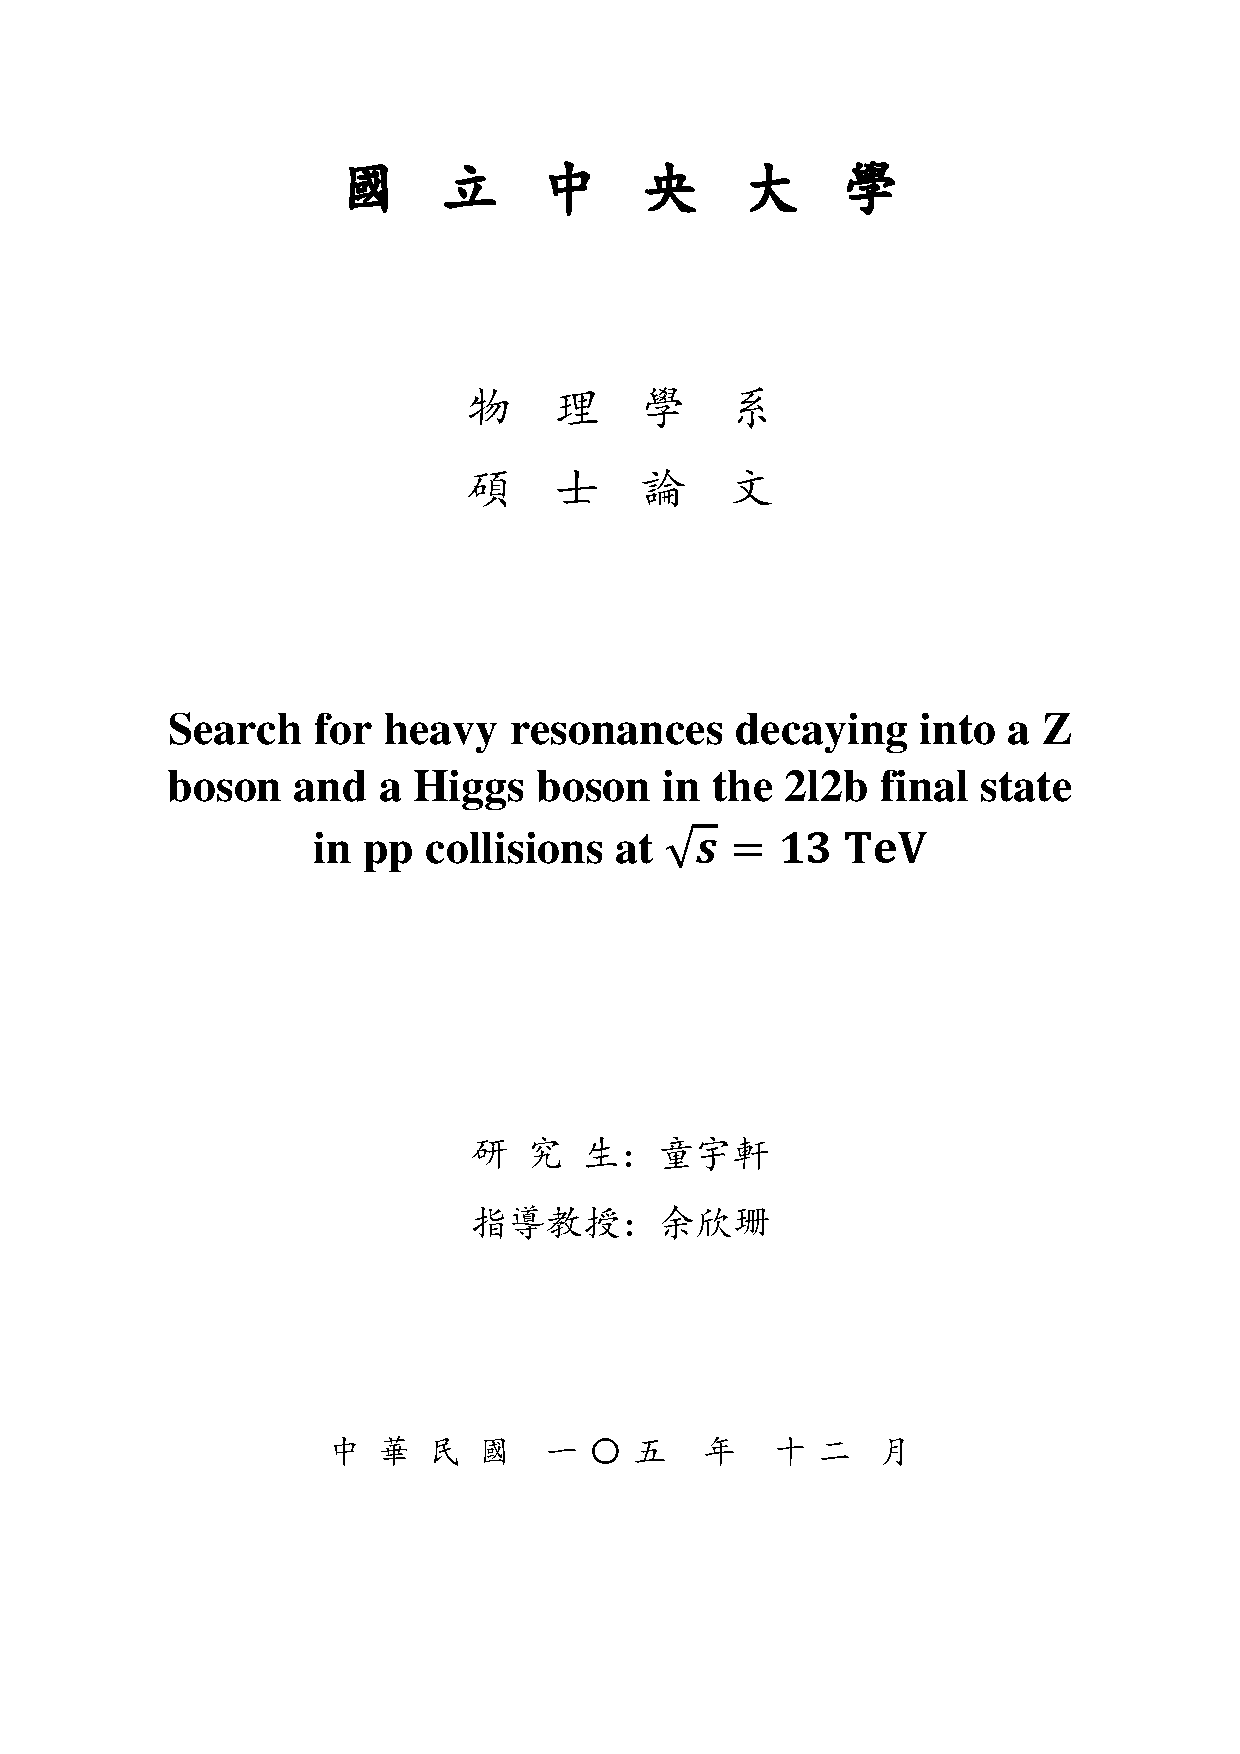
\includepdf{cover.pdf}
\afterpage{\blankpage} % Add a new blank page without page number


%----------------------------------------------------------------------------------------
%	TITLE PAGE
%----------------------------------------------------------------------------------------

\begin{titlepage}
  \begin{center} \setstretch{1.15}
    {\Large \bfseries \ttitle \par}
    \bigskip
    {\normalsize by \par}
    \bigskip
    {\large \authorname \par}
    \bigskip
    {\normalsize Submitted to the \deptname \par in partial fulfillment of the requirements for the degree of \par}
    \bigskip
    {\large \degreename \par}
    \bigskip    
    {at the \par}
    \bigskip
    {\large \MakeUppercase{\univname} \par}
    \bigskip
    {\normalsize November 2016 \par}
    \bigskip
    {\textcopyright \space \univname \space 2016. All rights reserved. \par}
    \bigskip \bigskip \bigskip 
    \begin{flushleft}
      {\large Author \dotfill \par}
    \end{flushleft}
    \begin{flushright} 
      {\deptname \par \today \par}
    \end{flushright}
    \begin{flushleft}
      {\large Certified by \dotfill \par}
    \end{flushleft}
    \begin{flushright} 
      {\supname \par Associate Professor \par Thesis Supervisor \par}
    \end{flushright}
    \begin{flushleft}
      {\large Accepted by \dotfill \par}
    \end{flushleft}
    \begin{flushright} 
      {\examname \par Professor \par Chairman, Thesis Committee \par}
    \end{flushright}
  \end{center}
\end{titlepage}

%\cleardoublepage

%----------------------------------------------------------------------------------------
%	ABSTRACT PAGE
%----------------------------------------------------------------------------------------

\begin{abstract} \setstretch{1.15}
%  \addchaptertocentry{\abstractname} % Add the abstract to the table of contents

  \noindent{\large \textbf{Abstract} \par}
  \bigskip
  \noindent{A search for heavy resonances decaying to a Higgs boson and a $Z$ boson is presented. The analysis is based on the data collected in 2015 with the CMS detector at a center-of-mass energy $\sqrt{s}$ = 13 TeV, corresponding to an integrated luminosity of 2.51 $fb^{-1}$. The Higgs bosons are reconstructed from high momentum $b\bar{b}$ quark pairs that are detected as a single massive jet, while the Z bosons are reconstructed from electron pairs and muon pairs. The analysis is separated in electron and muon channels, with single and double b-tag categories. A 95\% upper limit on the production cross section of $\sigma_{X}\times \mathcal{B}(X\rightarrow ZH)$ is derived from the combination of four categories with a limit of 0.063 $pb$ to 0.265 $pb$ for $m_X$ from 800 to 4000 GeV. \par}
  \bigskip
  \noindent{Thesis Supervisor: \space \supname \par}
  \noindent{Title: \space Associate Professor \par}
  
\end{abstract}

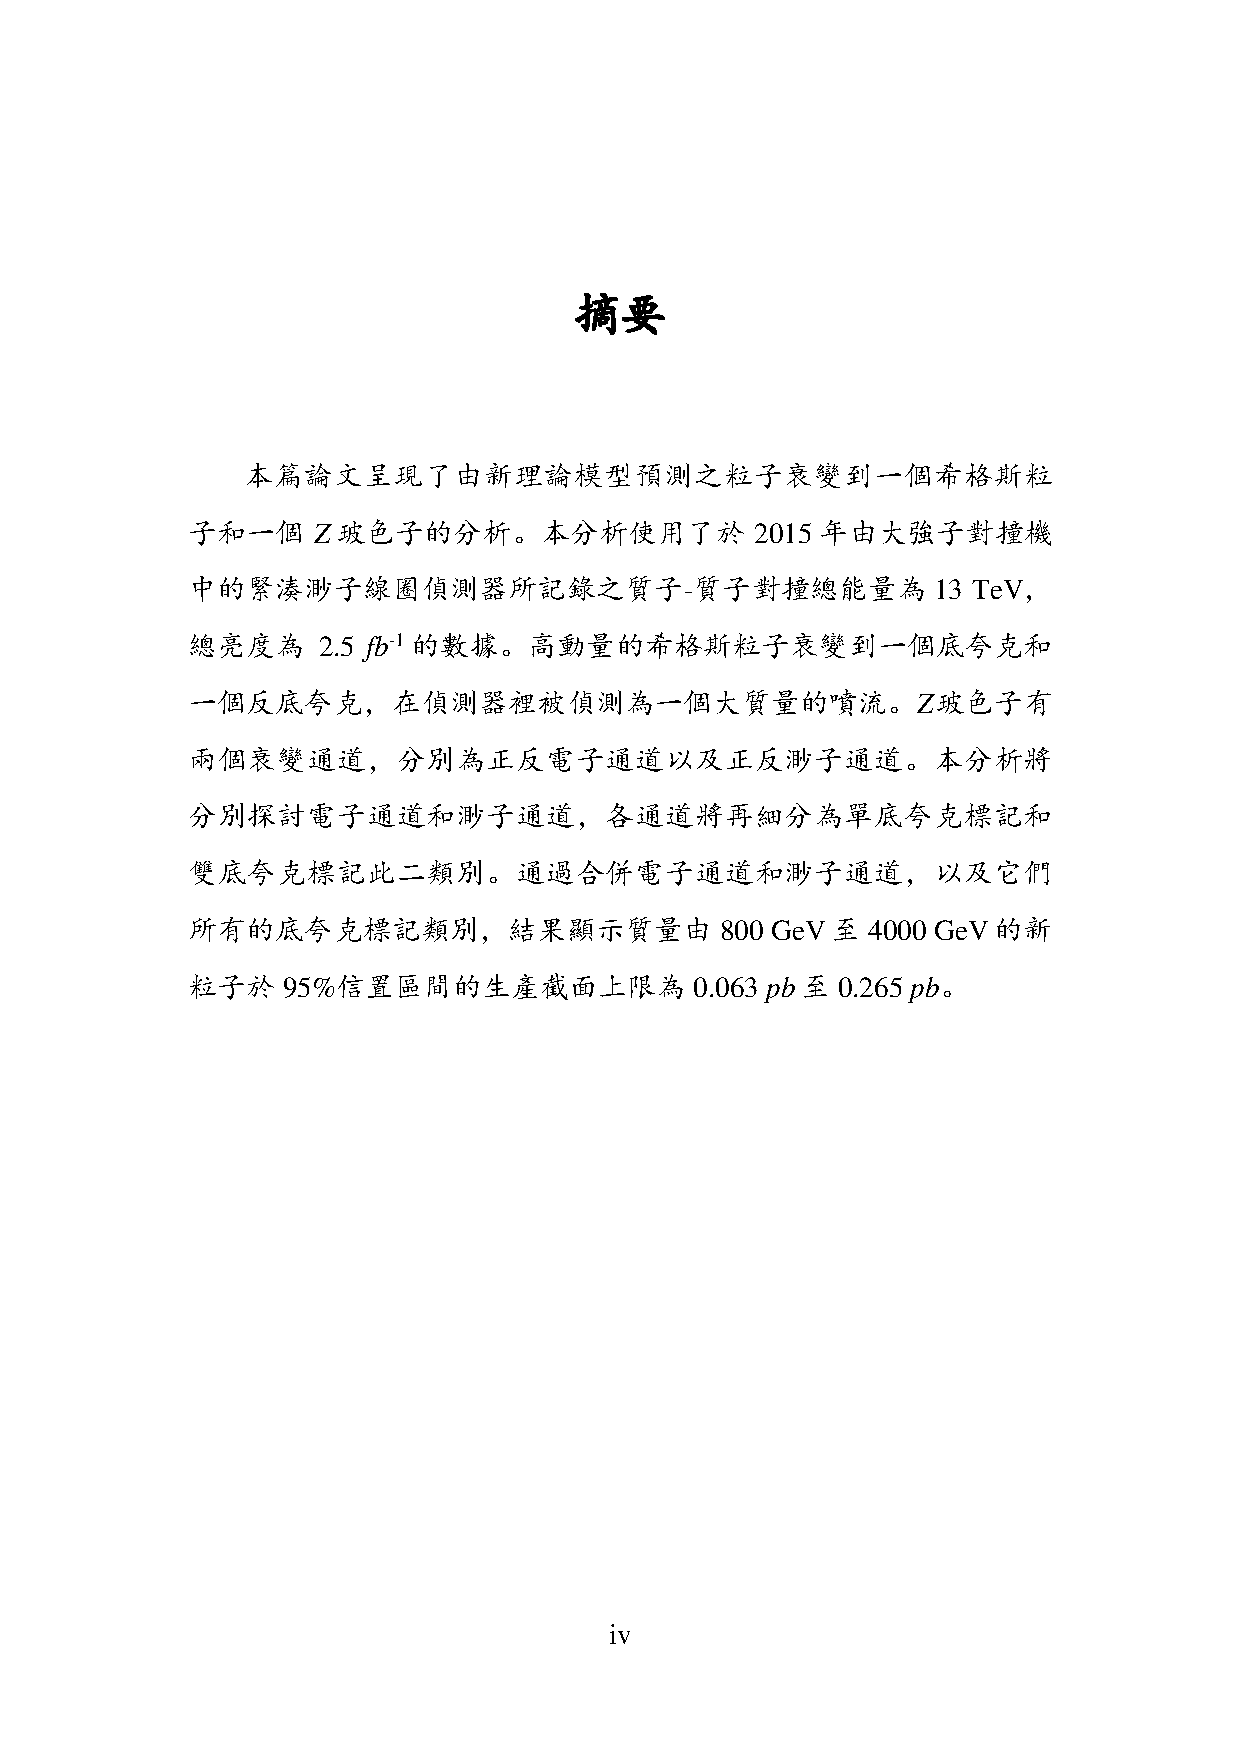
\includepdf{abstract.pdf}

%----------------------------------------------------------------------------------------
%	LIST OF CONTENTS/FIGURES/TABLES PAGES
%----------------------------------------------------------------------------------------

\tableofcontents % Prints the main table of contents
\listoffigures % Prints the list of figures
\listoftables % Prints the list of tables

%----------------------------------------------------------------------------------------
%	THESIS CONTENT - CHAPTERS
%----------------------------------------------------------------------------------------

\mainmatter % Begin numeric (1,2,3...) page numbering
\pagestyle{thesis} % Return the page headers back to the "thesis" style

% Include the chapters of the thesis as separate files from the Chapters folder
% Uncomment the lines as you write the chapters

\begin{linenumbers} %Turn line numbers on unless it is the final version
  
  %% Chapter 1

\newcommand{\tabhead}[1]{\textbf{#1}}
\newcommand{\mj}{$m_j$ }
\newcommand{\mzh}{$m_{ZH}$ }
\newcommand{\ttbar}{$t\bar{t}$ }
\newcommand{\Zjets}{$Z$+jets }
\newcommand{\Zee}{$Z\rightarrow e^+e^-$ }
\newcommand{\Zmm}{$Z\rightarrow \mu^+\mu^-$ }
\newcommand{\Hbb}{$H\rightarrow b\bar{b}$ }

\chapter{Introduction and Theory Overview} \label{Chapter1}

\section{Introduction}

This thesis presents the search of a heavy resonance decaying into a $Z$ boson and a Higgs boson at center-of-mass energy of 13 TeV using 2.51 $fb^{-1}$ proton-proton collision data collected with the CMS detector at the LHC. The $Z$ boson further decays into two charged leptons (electrons or muons), while the Higgs boson decays into two $b$ quarks. The Feymann diagram of the signal production is presented in Figure~\ref{fig:fey_signal}.

In this search, the high-momentum Higgs boson is reconstructed as a massive jet, and is identified by a b-tagging algorithm. The leptonic decay of $Z$ is considered in order to discriminate against the large multijet background. The heavy resonance signal appears as an excess in the spectrum of the invariant mass of the jet and the two leptons. This analysis is a part of the search for heavy resonances decaying into one vector boson plus one Higgs boson ($VH$)~\cite{Khachatryan:2016cfx}.

The organization of this thesis is described as follows. In the next section, a brief overview of Heavy Vector Triplets Model described by a simplified phenomenological Lagrangian is presented. A specific explicit model is then introduced, which is the benchmark model in this analysis. In Chapter~\ref{Chapter2}, an overview of the LHC and the CMS detector with its sub-detectors are presented. Chapter~\ref{Chapter3} reports the data sets and Monte Carlo samples used in this analysis. The reconstruction of physics objects and their selections are also described, and the agreement of data sets and Monte Carlo samples are presented. The estimation of backgrounds based on a data driven strategy is presented in Chapter~\ref{Chapter4}. In Chapter~\ref{Chapter5}, various systematic uncertainties are described. In Chapter~\ref{Chapter6}, the results of this analysis are discussed, and a conclusion is summarized.

\begin{figure}[t]
  \centering
  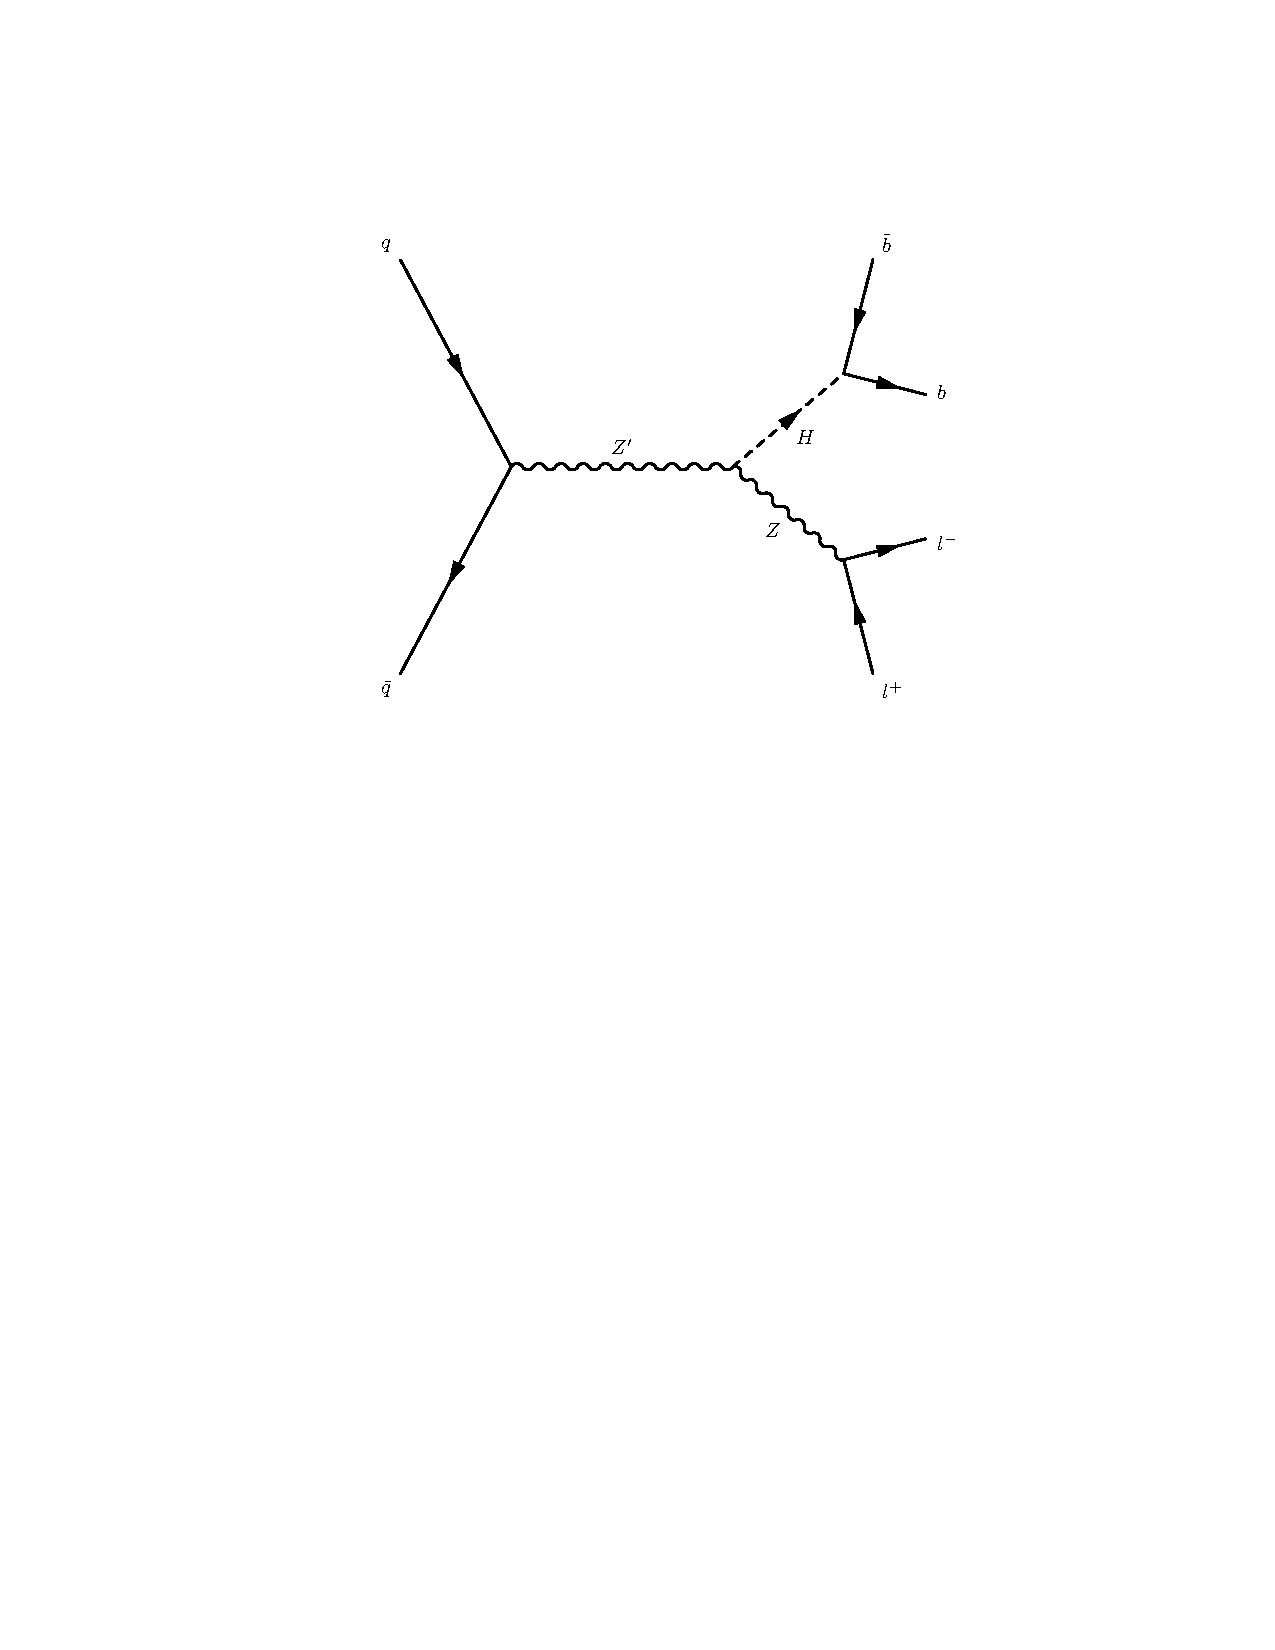
\includegraphics[width=1\textwidth,trim=0 400 0 100,clip=true]{Figures/feymann/qqZpZHllbb.pdf}
  \caption{Feymann diagram of the production of the heavy vector $Z'$, decaying into a $Z$ boson and a Higgs boson. The $Z$ boson further decays into two charged leptons, while the Higgs further decays into two $b$ quarks.}
  \label{fig:fey_signal}
\end{figure}

\section{Theoretical Motivations}

In the Standard Model (SM), the generation of masses for the weak gauge bosons ($W^\pm$ and $Z$) through electroweak symmetry breaking (EWSB) can be explained by the Higgs mechanism~\cite{PhysRevLett.13.508}. The mechanism was confirmed by the ATLAS and CMS experiments~\cite{Aad:2012tfa,Chatrchyan:2012xdj,Chatrchyan:2013lba} at the CERN 50 years after the theory has been proposed.

However, the discovered Higgs boson with mass of 125 GeV is much lighter than the Planck energy, which suggests that the SM may be incomplete. Various theories postulate the existence of new heavy resonances that couple to the SM bosons in an attempt to solve the hierarchy problem or naturalness problem. Some common models include the Little Higgs models~\cite{Han:2003wu,Perelstein:2005ka} and strongly coupled Composite Higgs~\cite{Contino:2011np,Marzocca:2012zn}. 

Various models can be generalized in the Heavy Vector Triplet (HVT) framework~\cite{Pappadopulo:2014qza}, which is a simplified approach based on a phenomenological Lagrangian. In the Simplified Model, only the relevant couplings and mass parameters are retained. The reason for this is that resonant searches are typically not sensitive to all the free parameters of the specific model, but only to those parameters that are related to the resonance mass and the interactions involved in its decay and production.

\subsection{Heavy Vector Triplet} \label{sec:hvtmodel}

Consider a heavy vector boson $V_\mu^a$, $a$ = 1,2,3, the simplified Lagrangian is described as
\begin{equation} \label{eq:simpleLag}
  \begin{aligned}
    \mathcal{L}_V = &-\frac{1}{4}D_{[\mu}V_{\nu]}^aD^{[\mu}V^{\nu]a}+\frac{m_V^2}{2}V_\mu^aV^{\mu a}\\
    &+ig_Vc_HV_\mu^aH^\dagger\tau^a\bar{D}^\mu H+\frac{g^2}{g_V}c_FV_\mu^a\sum\limits_{f}\bar{f}_L\gamma^\mu\tau^af_L\\
    &+\textup{quadrilinear terms}
  \end{aligned}
\end{equation}

The first term\footnote{The term \(D_{[\mu}V_{\nu]}^a = D_\mu V_\nu^a - D_\nu V_\mu^a\), where \(D_\mu V_\nu^a = \partial_\mu V_\nu^a + g\varepsilon^{abc}W_\mu^bV_\nu^c\).} in Eq.~\ref{eq:simpleLag} describes the interactions of $V$ with the SM weak bosons. The second term in the equation is the interactions of $V$ with itself, where the mass parameter $m_V$ does not coincide with the physical mass of the resonances. The third and fourth terms of the equation contains the interactions of $V$ with the Higgs current\footnote{The Higgs current term \(iH^\dagger\tau^a\bar{D}^\mu H = iH^\dagger\tau^aD^\mu H - iD^\mu H^\dagger\tau^aH\).} and with the SM left-handed fermionic currents\footnote{The fermionic currents \(\sum\bar{f}_L\gamma^\mu\tau^af_L\) involve the interactions of $V$ to leptons, light quarks and the third quarks family.}, respectively. The quadrilinear terms\footnote{The quadrilinear terms can be written as \[\frac{g_V}{2}c_{VVV}\varepsilon_{abc}V_\mu^aV_\nu^bD^{[\mu}V^{\nu]c} + g_V^2c_{VVHH}V_\mu^aV^{\nu a}H^\dagger H - \frac{g}{2}c_{VVW}\varepsilon_{abc}W^{\mu\nu a}V_\mu^bV_\nu^c.\]} do not contribute directly to $V$ decays and single production processes, therefore these terms can be disregarded.

In Eq.~\ref{eq:simpleLag}, besides the $SU$(2)$_L$ coupling constant $g$, another coupling constant $g_V$ is introduced to represent the strength of $V$ interactions. In addition, the term $c_H$ describes the $V$ interactions with the SM vector bosons and with the Higgs. Similarly, the term $c_F$ describes the $V$ interactions with fermions. They are expected to be of the order of unity in most models. 

\subsubsection*{Masses}

After the EWSB, only the photon stays massless due to the unbroken $U$(1)$_{EM}$, while the weak bosons acquire a mass and a mixing with heavy vector $V$. The mass matrix of the ($Z$, $V^0$) and the ($W^\pm$, $V^\pm$) are 
\begin{equation} \label{eq:matrixN}
  \mathcal{M}_N^2 =
  \begin{pmatrix}
    \hat{m}_Z^2 &
    c_H\xi\hat{m}_Z\hat{m}_V \\
    c_H\xi\hat{m}_Z\hat{m}_V &
    \hat{m}_V^2 \\
  \end{pmatrix}
\end{equation}
and
\begin{equation} \label{eq:matrixC}
  \mathcal{M}_C^2 =
  \begin{pmatrix}
    \hat{m}_W^2 &
    c_H\xi\hat{m}_W\hat{m}_V \\
    c_H\xi\hat{m}_W\hat{m}_V &
    \hat{m}_V^2 \\
  \end{pmatrix}
\end{equation}
respectively, where
\[\hat{m}_Z = \frac{e}{2\sin\theta_W\cos\theta_W}\hat{v}\]
\[\hat{m}_W = \cos\theta_W\hat{m}_Z\]
\[\hat{m}_V^2 = m_V^2 + g_V^2c_{VVHH}\hat{v}^2\]
\[\xi = \frac{g_V\hat{v}}{2\hat{m}_V}\]
Note that $e \approx \sqrt{4\pi/137}$, $\hat{v}$ is the Higgs field Vacuum Expectation Value, which has a value of 246 GeV, and $\theta_W$ is the weak mixing angle.

By taking the determinant of the mass matrices in Eq.~\ref{eq:matrixN} and Eq.~\ref{eq:matrixC}, the relation of the physical masses $M$ between charged and neutral heavy vectors are connected by $\theta_W$.
\begin{equation}
  m_W^2M_\pm^2 = \cos^2\theta_Wm_Z^2M_0^2
\end{equation}

In the experimental searches, the masses of new vectors should be at or above TeV scale, but the masses of SM bosons $m_{W,Z}$ should be preserved at about 100 GeV. A hierarchy in the mass spectrum is required to have
\begin{equation} \label{eq:massLimit}
  \frac{\hat{m}_{W,Z}}{\hat{m}_V} \sim \frac{m_{W,Z}}{M_{\pm,0}} \ll 1
\end{equation}

Under the limit in Eq.~\ref{eq:massLimit}, by expanding the determinant of the mass matrices in Eq.~\ref{eq:matrixN} and Eq.~\ref{eq:matrixC}, a simple approximate expressions for $m_W$ and $m_Z$ are given by
\[m_Z^2 \approx \hat{m}_Z^2(1-c_H^2\xi^2)\]
\[m_W^2 \approx \hat{m}_W^2(1-c_H^2\xi^2)\]
Since $\hat{m}_W = \cos\theta_W\hat{m}_Z$, the $W$-$Z$ mass ratio is given by 
\begin{equation} \label{eq:weakMass}
  \frac{m_W^2}{m_Z^2} \simeq \cos^2\theta_W
\end{equation}

Experimentally, the value of $\cos^2\theta_W$ is about 0.77. The charged and neutral $V$s are degenerated by
\begin{equation} \label{eq:hvtMass}
  M_\pm^2 = M_0^2 (1+\mathcal{O}(\%))
\end{equation}

It is clear that the mass splitting of charged and neutral states of $V$ is small enough to be ignored. This implies that the two states have comparable production rates.

\subsubsection*{Decay Widths}

Given that the mixing angles between weak bosons and $V$ are small due to the hierarchy in the mass spectrum, the couplings of the neutral and charged $V$ to left- and right-handed fermion chiralities can be written as
\begin{equation} \label{eq:LRcoupling}
  \begin{cases}
    g_L^N \simeq\frac{g^2}{g_V}\frac{c_F}{2}, \quad g_R^N \simeq 0 \\
    g_L^C \simeq\frac{g^2}{g_V}\frac{c_F}{\sqrt{2}}, \quad g_R^C = 0
  \end{cases}
\end{equation}
The ($g_{L,R}^{W,Z}$)$_{SM}$ in the Eq.~\ref{eq:LRcoupling} is the ordinary SM $W$ and $Z$ couplings with a normalization of $g_L^W = g/\sqrt{2}$. The $g$ is electroweak coupling which has a value of 0.65.

The decay width $\Gamma$ for fermionic channels can be written as
\begin{equation} \label{eq:fermionWidth}
  \Gamma_{V_\pm\rightarrow f\bar{f}'} \simeq 2\Gamma_{V_0\rightarrow f\bar{f}} \simeq N_c[f](\frac{g^2c_F}{g_V})^2\frac{M_V}{48\pi}
\end{equation}
where $N_c[f]$ is the number of colors (3 for di-quarks and 1 for di-leptons). The parameters $c_F={c_l,c_q,c_3}$ control the relative branching ratios (BR) to leptons, light quarks and the third family quarks.

The decay width for bosonic channels are
\begin{equation} \label{eq:bosonWidth}
  \Gamma_{V_0\rightarrow W_L^+W_L^-}\simeq\Gamma_{V_\pm\rightarrow W_L^\pm Z_L}\simeq\Gamma_{V_0\rightarrow Z_Lh}\simeq\Gamma_{V_\pm\rightarrow W_L^\pm h}\simeq\frac{g_V^2c_H^2M_V}{192\pi}[1+\mathcal{O}(\xi^2)]
\end{equation}
The channels that are not reported in the Eq.~\ref{eq:fermionWidth} and Eq.~\ref{eq:bosonWidth} are either forbidden or suppressed.

Since the $M_V$ is in the order of TeV scale, the $\xi$ should be very small. In this case, for a given resonance mass, the decay widths are fixed by the couplings $g^2c_F/g_V$ and $g_Vc_H$. The BRs and the production rate are controlled by the two parameters $g^2c_F/g_V$ and $g_Vc_H$.

\begin{figure}[t]
  \centering
  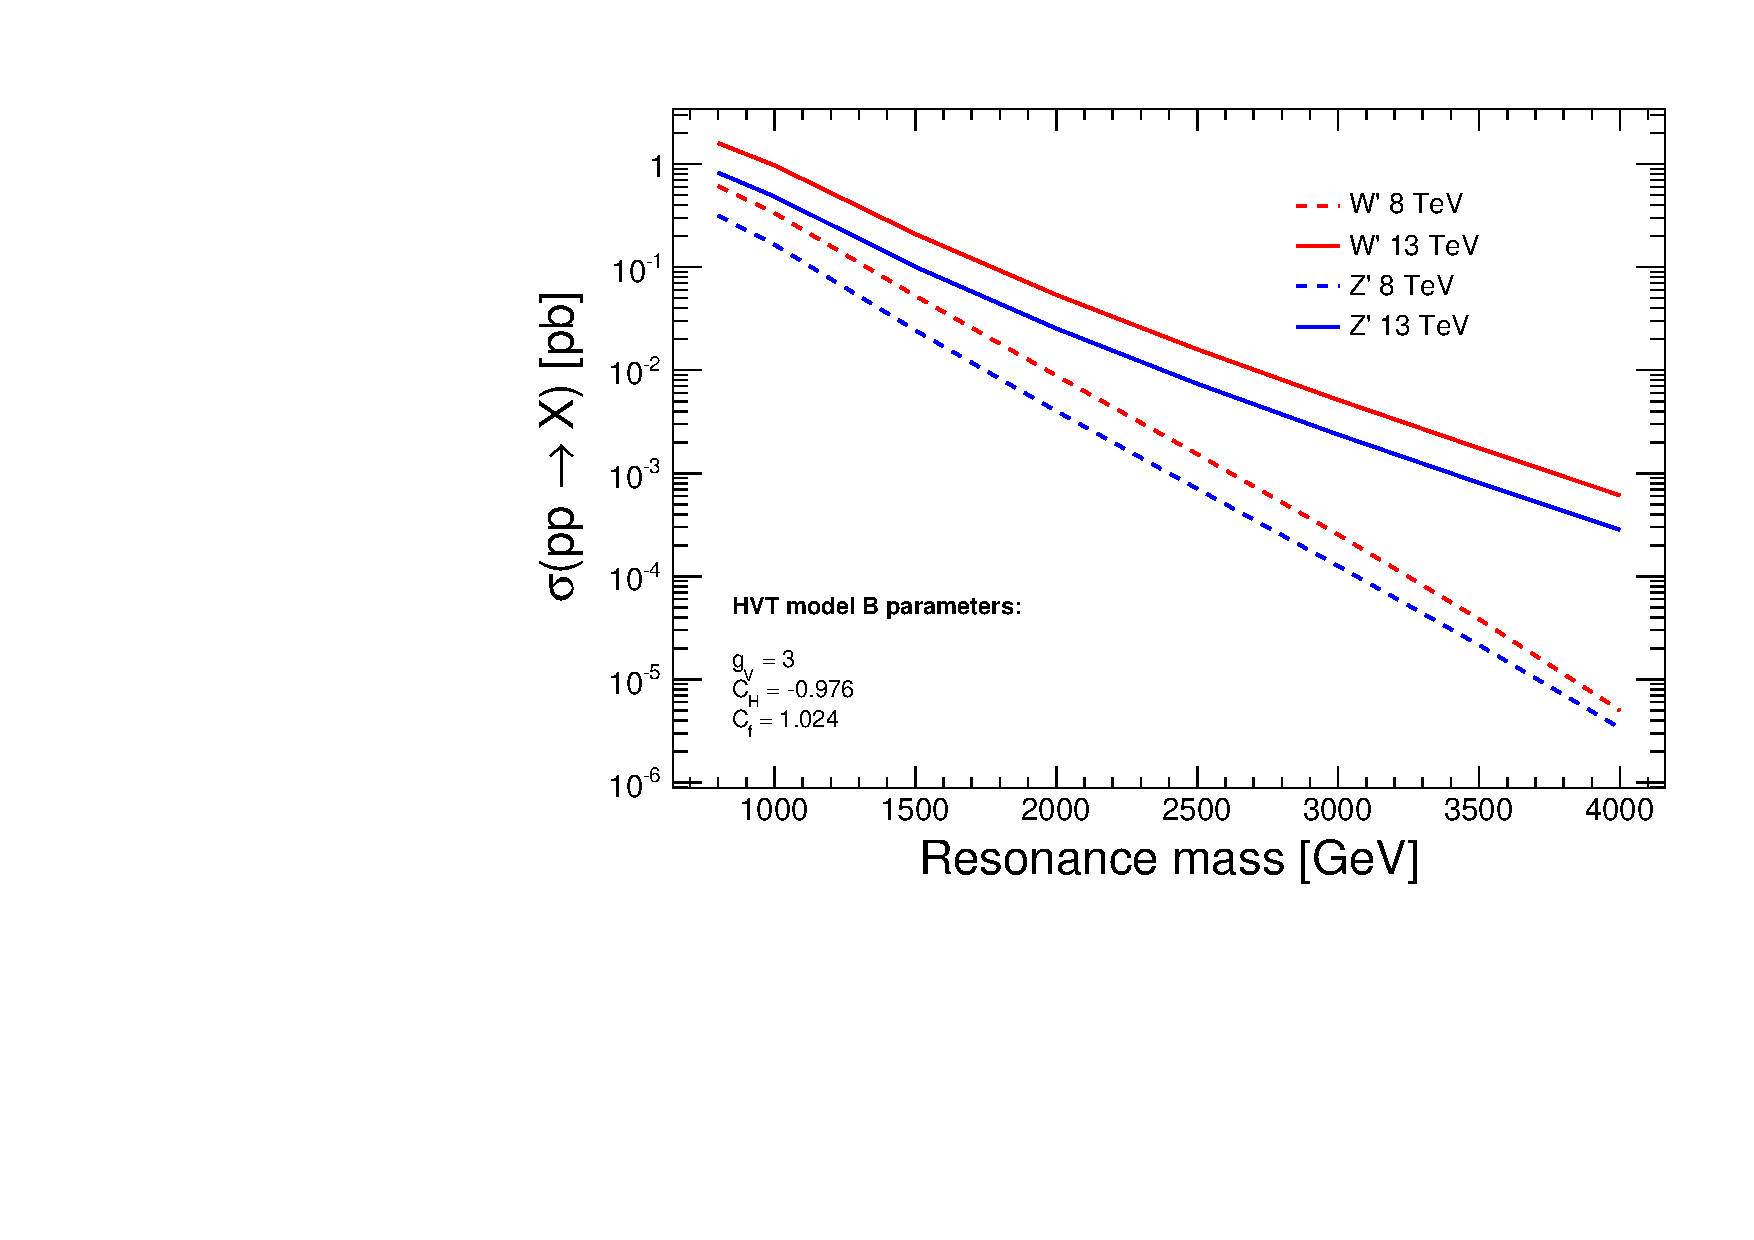
\includegraphics[width=0.55\textwidth]{Figures/hvt-xsec.pdf}
  \caption{Theoretical production cross section as a function of resonance mass for HVT Minimal Composite Higgs Model.}
  \label{fig:hvt_xsec}
\end{figure}

\subsection{Explicit Model} \label{sec:modelb}

It is now clear that the explicit model can be entirely described in terms of the two couplings $g^2c_F/g_V$ and $g_Vc_H$ and the mass $M_V$ with a good approximation~\cite{Pappadopulo:2014qza}.

Consider a strongly coupled scenario, so called Minimal Composite Higgs Model, where the Higgs doublet emerges from the spontaneous symmetry breaking of a global $SO$(5) symmetry to an $SO$(4) subgroup. In this scenario, the parameters $c_H$ and $c_F$ are fixed, \[c_H \sim -1, \quad c_F \sim 1\]

In addition, $g_V \gtrsim$ 3 is set to represent the strong coupling. In this case, the dominant BRs are bosonic decays due to $g_Vc_H \simeq -g_V$ in Eq.~\ref{eq:bosonWidth}, while the fermionic decays are extremely suppressed due to $g^2c_F/g_V \simeq g^2/g_V$ in Eq.~\ref{eq:fermionWidth}.

The results of this model is particularly interesting for the present search, since it predicts signal cross sections in the order of $fb$ for resonances up to 2$\sim$3 TeV (Figure~\ref{fig:hvt_xsec}), branching ratios to vector bosons close to the unity (Figure~\ref{fig:hvt_brs}), and thus being accessible at the LHC Run-II.

If the coupling is very large (for example $g_V$ = 8), the total width will be increased since the width of decays to dibosons grows with $g_V$ from Eq.~\ref{eq:bosonWidth}. But a very large coupling leads to an extremely broad resonance, which is not interesting to the experimental searches for a narrow resonance. Therefore, the $g_v$ has been constrained by $g_V \lesssim 4\pi$.

\begin{figure}[t]
  \centering
  \begin{tabular}{cc}
    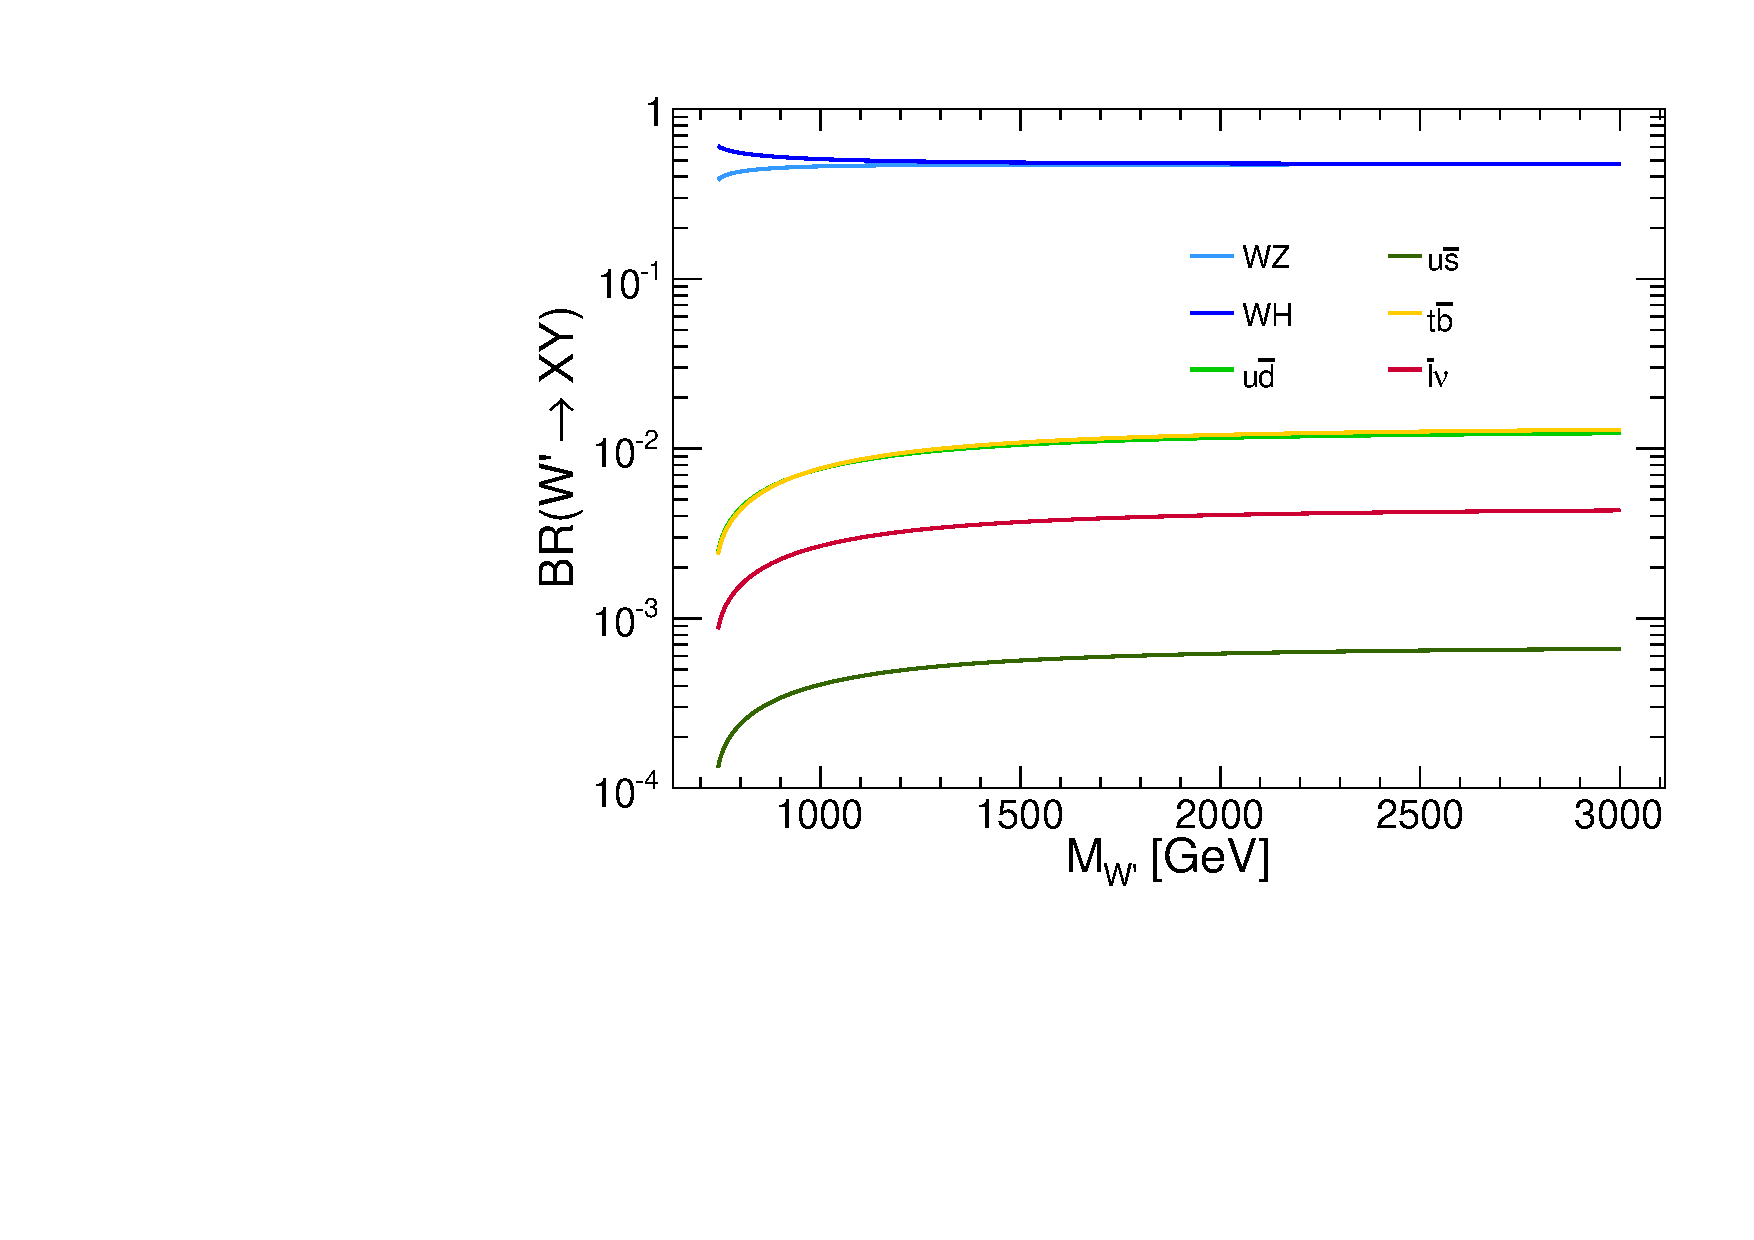
\includegraphics[width=0.5\textwidth]{Figures/hvt-wp-brs.pdf} &
    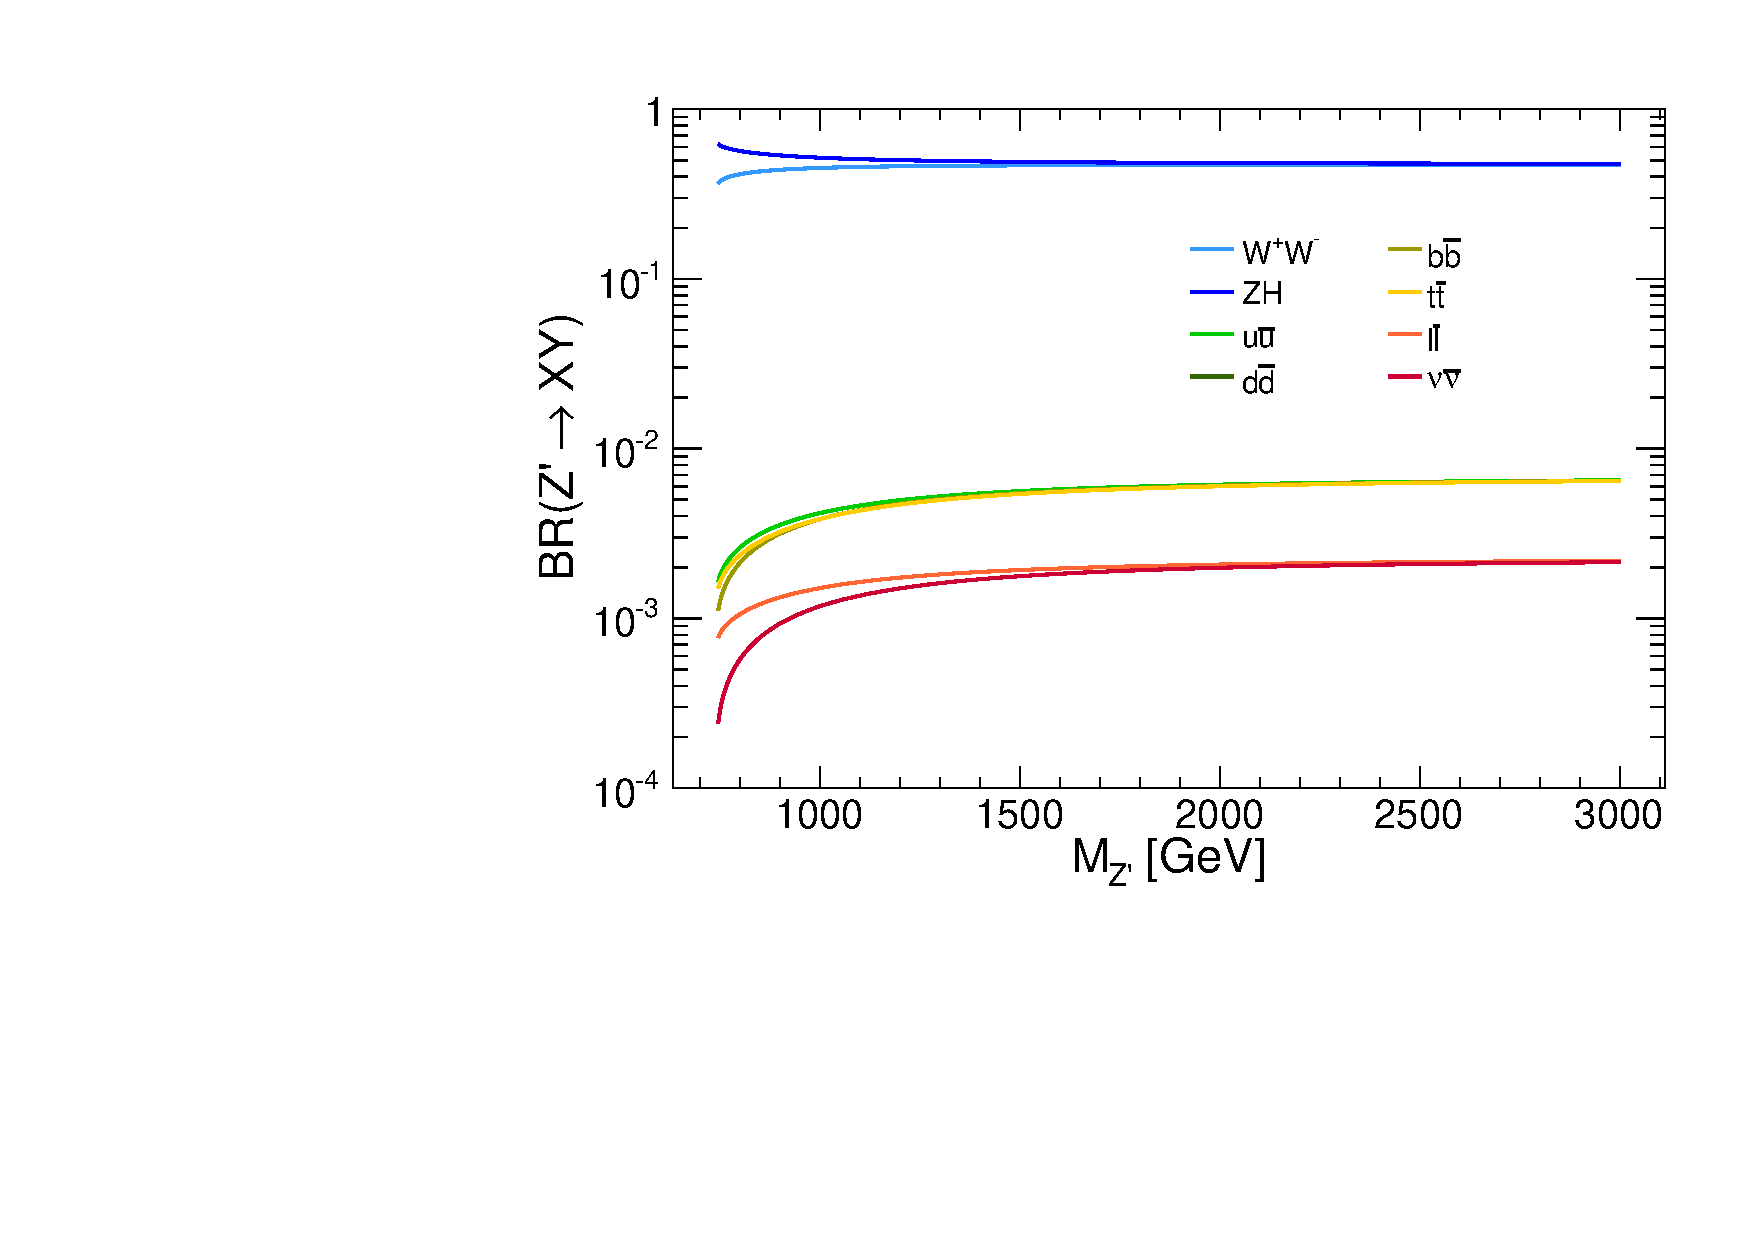
\includegraphics[width=0.5\textwidth]{Figures/hvt-zp-brs.pdf} \\
  \end{tabular}
  \caption{Branching ratios as a function of the resonance mass for a W' (left) and Z' (right) in the HVT Minimal Composite Higgs Model.}
  \label{fig:hvt_brs}
\end{figure}

  %\include{Chapters/Chapter2} 
  %\include{Chapters/Chapter3}
    \chapter{Introduction and Theory Overview} \label{chap:1}

\section{Introduction}
The analysis is aim at searching for heavy resonances decaying to a pair of Higgs
bosons in the four b quark final state using 35.9$fb^{-1}$ proton-proton collison data at center-of-mass energy 13 TeV collected with the CMS detector at the LHC. The figure 1.1 shows the feynman diagram of the channel. 

The Higgs tagging process uses the b-tagging algorithm, N-subjetness variable, and the mass of the jets. The analysis is searching for a bump in the dominant background of multi-jet events.


\begin{figure}[t]
  \begin{center}

    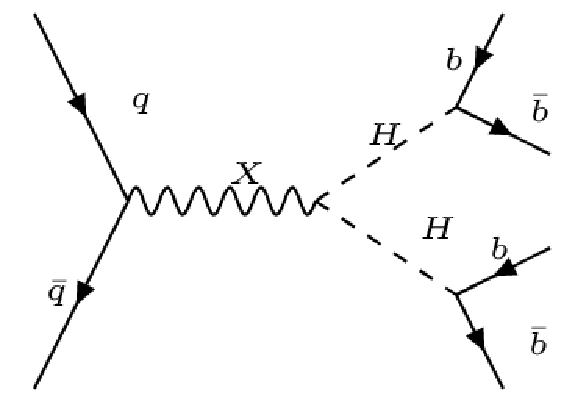
\includegraphics[width=0.5\textwidth]{Figures/Screenshot_20170601_160641.pdf} 
    \end{center}
  \caption{The feynman diagram of q$\bar{q}$ $\rightarrow$ X $\rightarrow$ HH $\rightarrow$ $b\bar{b}b\bar{b}$.}
\end{figure}

In \autoref{chap:1}, an overview of Wrapped Extra Dimension theory, signal model, and motivation is presented. In \autoref{chap:2}, the LHC and the CMS detector are simply introduced. In \autoref{chap:3}, the information of the data and the Monte Carlo Simulation is shown along with the comparison of shape of each discripant variable. The reconstruction and the selection of the event is also fully detailed. In \autoref{chap:4}, the background estimation method based on data driven is presented. All sysyematic uncertainted considered is documented in \autoref{chap:5}. Finally, the result of 95$\% $ CL$_{s}$ upper limit of cross section $\times$ branch ratio is shwon in \autoref{chap:6}. 

\section{Theory}
%http://dx.doi.org/10.1016/j.physletb.2012.08.021
%http://www.sciencedirect.com/science/article/pii/S037026931200857X

The discovery of the boson whose mass around 125 GeV and with properties close to Higgs mechanism in the Standard model has incited the search under Higgs potential including Higgs self-coupling\citep{jetarea_fastjet_pu,HiggsdiscoveryAtlas}. Especially, it is a worth explored channel to finding new physic beyond Standard model. 
Targeting heavy resonance, the model Wrapped Extra Dimension is considered. 

\subsection{Wraped Extra Dimension} 

%https://journals.aps.org/prl/pdf/10.1103/PhysRevLett.83.3370
To solve the hierarchy problem, Wrapped Extra dimension proposed by Randall and Sundrum postulates a scenario that the SM particles and forces associating with gravity force are confined to a four-dimension subspace within (4+n)-dimension spacetime, referred to as "3-brane", 
to explain the fact that we do not see experimental signs of the extra dimensions\citep{Randall:1999ee}.  The spacetime metrix takes the form\citep{Oliveira:2014kla}:

\begin{equation} \label{eq1}
\begin{split}
ds^2 = e^{-2\sigma(\phi)}\eta_{\mu\nu}dx^{\mu}dx^{\nu} + r^2_{c}d\phi^2, 
\end{split}
\end{equation}
where $\mu$ and $\nu$ run over 1, 2, 3, and 4, and $\phi$ is the fifth dimension. Its classical action is 

\begin{equation} \label{eq1}
\begin{split}
S = S_{Gravity}+S_{TeV}+S_{Planck}+S_{Matter},
\end{split}
\end{equation},
where $S_{Gravity}$ is the action of bulk gravity, and $S_{Matter}$ is the action of matter field. The actions can be written as:

\begin{equation} \label{eq1}
\begin{split}
S_{i=TeV/Planck}=-\int d^4x \sqrt{g(\phi =0,\pi)}\Lambda_{i=TeV/Planck}\\
S_{Gravity}=\int d^4 \int ^{\pi}_{\pi} d\phi \sqrt{g}(-\Lambda_{bulk}+2M^3_{5}R),
\end{split}
\end{equation}
where $\Lambda$ is hte vacuum energy density, R is Ricci metrix. We arrive at:

\begin{equation} \label{eq1}
\begin{split}
\sigma(\phi)=r_{c}|\phi | \sqrt{\frac{-\Lambda}{24M^2_5}}\equiv r_c|\phi |k \\
k\equiv  \sqrt{\frac{-\Lambda}{24M^2_5}}, \\
\end{split}
\end{equation}
where k is referred as curvature factor. We can integrate the fifth dimension and get four-dimension Planck mass: 
\begin{equation} \label{eq1}
\begin{split}
\bar{M}^2_{Pl}=\frac{M^3_5}{k}(1=e^{-2\pi kr_c}).
\end{split}
\end{equation}

Finally, we get the spacetime metrix:  
\begin{equation} \label{eq1}
\begin{split}
ds^2 = e^{-2kr_c\phi}\eta_{\mu\nu}dx^{\mu}dx^{\nu} + r^2_{c}d\phi^2, 
\end{split}
\end{equation}


where k is a scale of the order of the Planck scale, xm are
coordinates for the familiar four dimensions, while 0 $\leq$ $\phi$ $\leq$ $\pi$ is the coordinate for an extra dimension, which is
a finite interval whose size is set by $r_c$. The exponential is the source of large hierarchy between weak and the observed Planck scale.  


%https://journals.aps.org/prl/pdf/10.1103/PhysRevLett.83.4922
%https://arxiv.org/pdf/hep-ph/9911406.pdf

%https://arxiv.org/pdf/hep-ph/9909255.pdf
%https://arxiv.org/pdf/hep-ph/0701186.pdf
%https://arxiv.org/pdf/hep-ph/0701150.pdf
There are models predicting the existence of new particles, such as spin-0 radion and spin-2 graviton\citep{Davoudiasl:1999jd,Agashe:2007zd,Fitzpatrick:2007qr}. For example, a radion scalar is added to stablize the $r_c$ in RS theory without a fune-tuning of parameters\citep{Goldberger:1999uk}. Other model proves that
a radion field can remove the constraints between two branes without a stablized radius\citep{Csaki:1999mp}, and that 
%https://arxiv.org/pdf/hep-th/0008151.pdf
a radion scalar can exist with radus stabilization in bulk scalar field while assuming stabilization exists\citep{Csaki:2000zn}.
A possible mixing of the radion which is the only graviscalar in RS model and the Higgs is proposed\citep{Giudice:2000av}.
%https://arxiv.org/pdf/hep-ph/0002178.pdf
However, according to the latest experimental data, the mixing is expected to be small. Therefore, the contribution of the mixing is not considered in this analysis\citep{Desai:2013pga}.
%https://arxiv.org/pdf/1307.3765.pdf

We follow the ref.\citep{Agashe:2013kyb} to calculate the cross section of bulk graviton.
\begin{equation} \label{eq1}
\begin{split}
gg \rightarrow KK graviton \rightarrow ZZ, WW, hh (and t\bar{t}, b\bar{b}) \\
\textit{L}_{prod.} = 0.053 (\frac{k}{M_{Pl}M_{G}})\eta^{\mu\alpha}\eta^{\nu\beta}h^{(1)}_{\alpha\beta}T^{gluon}_{\mu \nu}(x), 
\end{split}
\end{equation}
where the $M_G$ is the mass of KK graviton, and $T^{gluon}_{\mu \nu}$ is four-dimesion four-momentum of SM gluon. The implementation of the calcuation is described in ref.\citep{Oliveira:2014kla}. The model which is capable of calculating the correction of next-to-leading-order QCD induced spin-2 particle is used. The cross section is calculated by \textsf{MG5\_aMC@NLO}.
Because of the Higgs-like property of radion, the cross section of radion is calculated by rescaling the cross section of Higgs like particle\citep{Agashe:2013kyb,AN-16-300}. The production of Higgs-like particle by gluon-gluon fusion is followed by ref.\citep{Catani:2003zt,Heinemeyer:2013tqa}, which is calcuated in next-to-next-to-leading-order QCD induced soft-gluon resummation. The Higgs-like calculation is up to 1 TeV, and it is constant for mass above 1 TeV. The cross section of radion is based on the cross section of Higgs-like multiplied by k factor. 
In the calcuation of both signal, CTEQ6LPDF is used\citep{Nadolsky:2008zw}.  

\subsection{Motivation} 
%https://arxiv.org/pdf/1512.04357.pdf
There are models predicting heavy resonances decaying into VV\citep{Brehmer:2015dan}.
%https://arxiv.org/abs/1506.00962
%https://arxiv.org/abs/1503.04677
%https://arxiv.org/abs/1409.6190
%https://arxiv.org/abs/1405.1994
Several researches on these channels are performed in both CMS and ATLAS.
There are also the combinations of these analyses\citep{Khachatryan:2014hpa,ATLASZV,ATLASWV,ATLASVV}.
%https://arxiv.org/abs/1405.3447
%https://arxiv.org/abs/1512.05099
The combination from ATLAS excludes the resonance of Bulk Graviton from below 810 GeV\citep{Aad:2015ipg}, and despit the combination from CMS fails to exclude any mass spectum of Bulk Graviton given a less sensitive model, it sets the upper limit of 10 fb of cross section of Bulk Graviton through $M_X$ from 600 to 2500 GeV\citep{CMSZVWV}.
%https://arxiv.org/pdf/1503.04114.pdf
%https://arxiv.org/pdf/1506.00285.pdf
Besides, searches for Bulk Graviton decaying into HH in four b-flavored quarks final state have been perfromed by CMS and ATLAS at $\sqrt{s}$ = 8 TeV\citep{Khachatryan:2015year,Aad:2015uka}. They exlude the mass region below 830 and 720 GeV respectively. The intermediate region of the mass of heavy resonances ( $M_X \thickapprox$ 2 TeV ) is left interesting to be explored.
 



%
%\begin{figure}[t]
%  \centering
%  \begin{tabular}{cc}
%    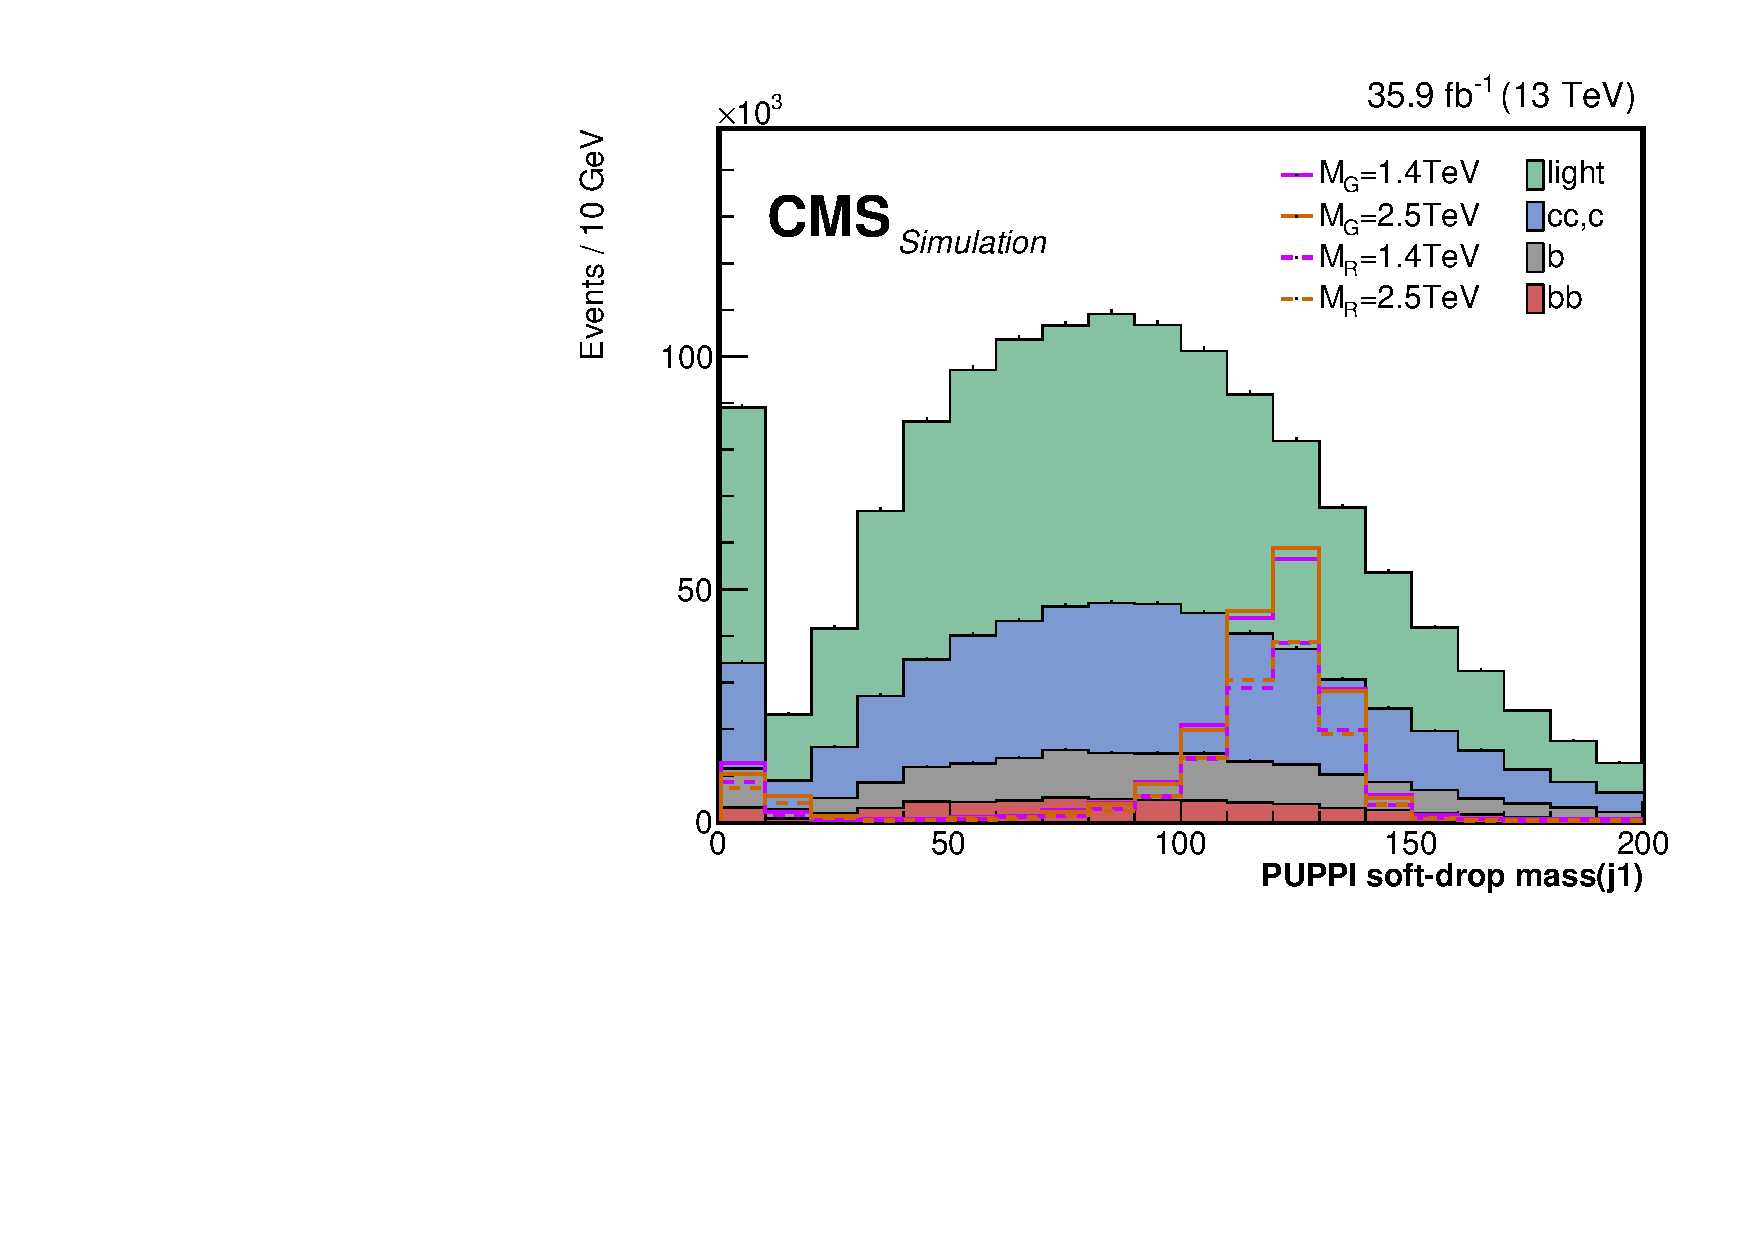
\includegraphics[width=0.5\textwidth]{Figures/MC_N1/puppiSDMassThea_j0.pdf} &
%    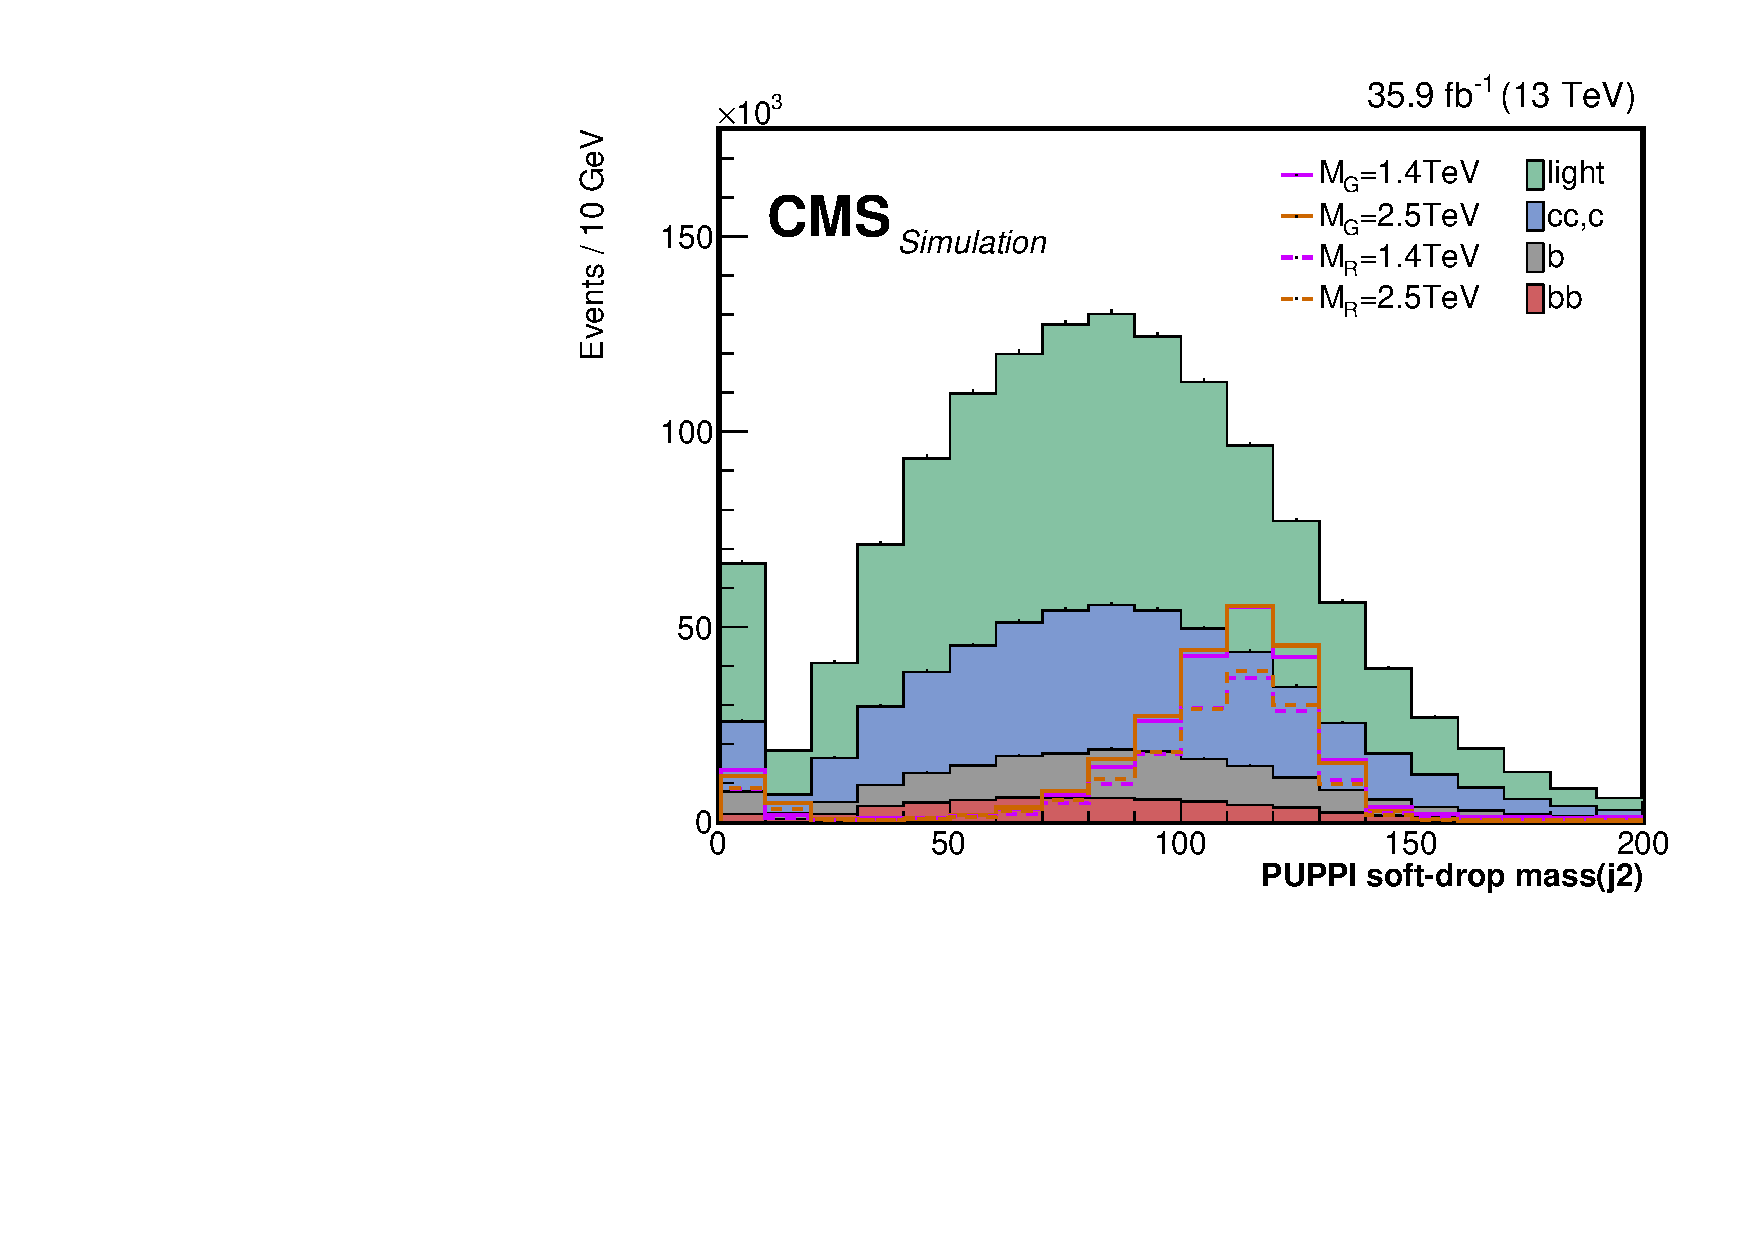
\includegraphics[width=0.5\textwidth]{Figures/MC_N1/puppiSDMassThea_j1.pdf} \\
%     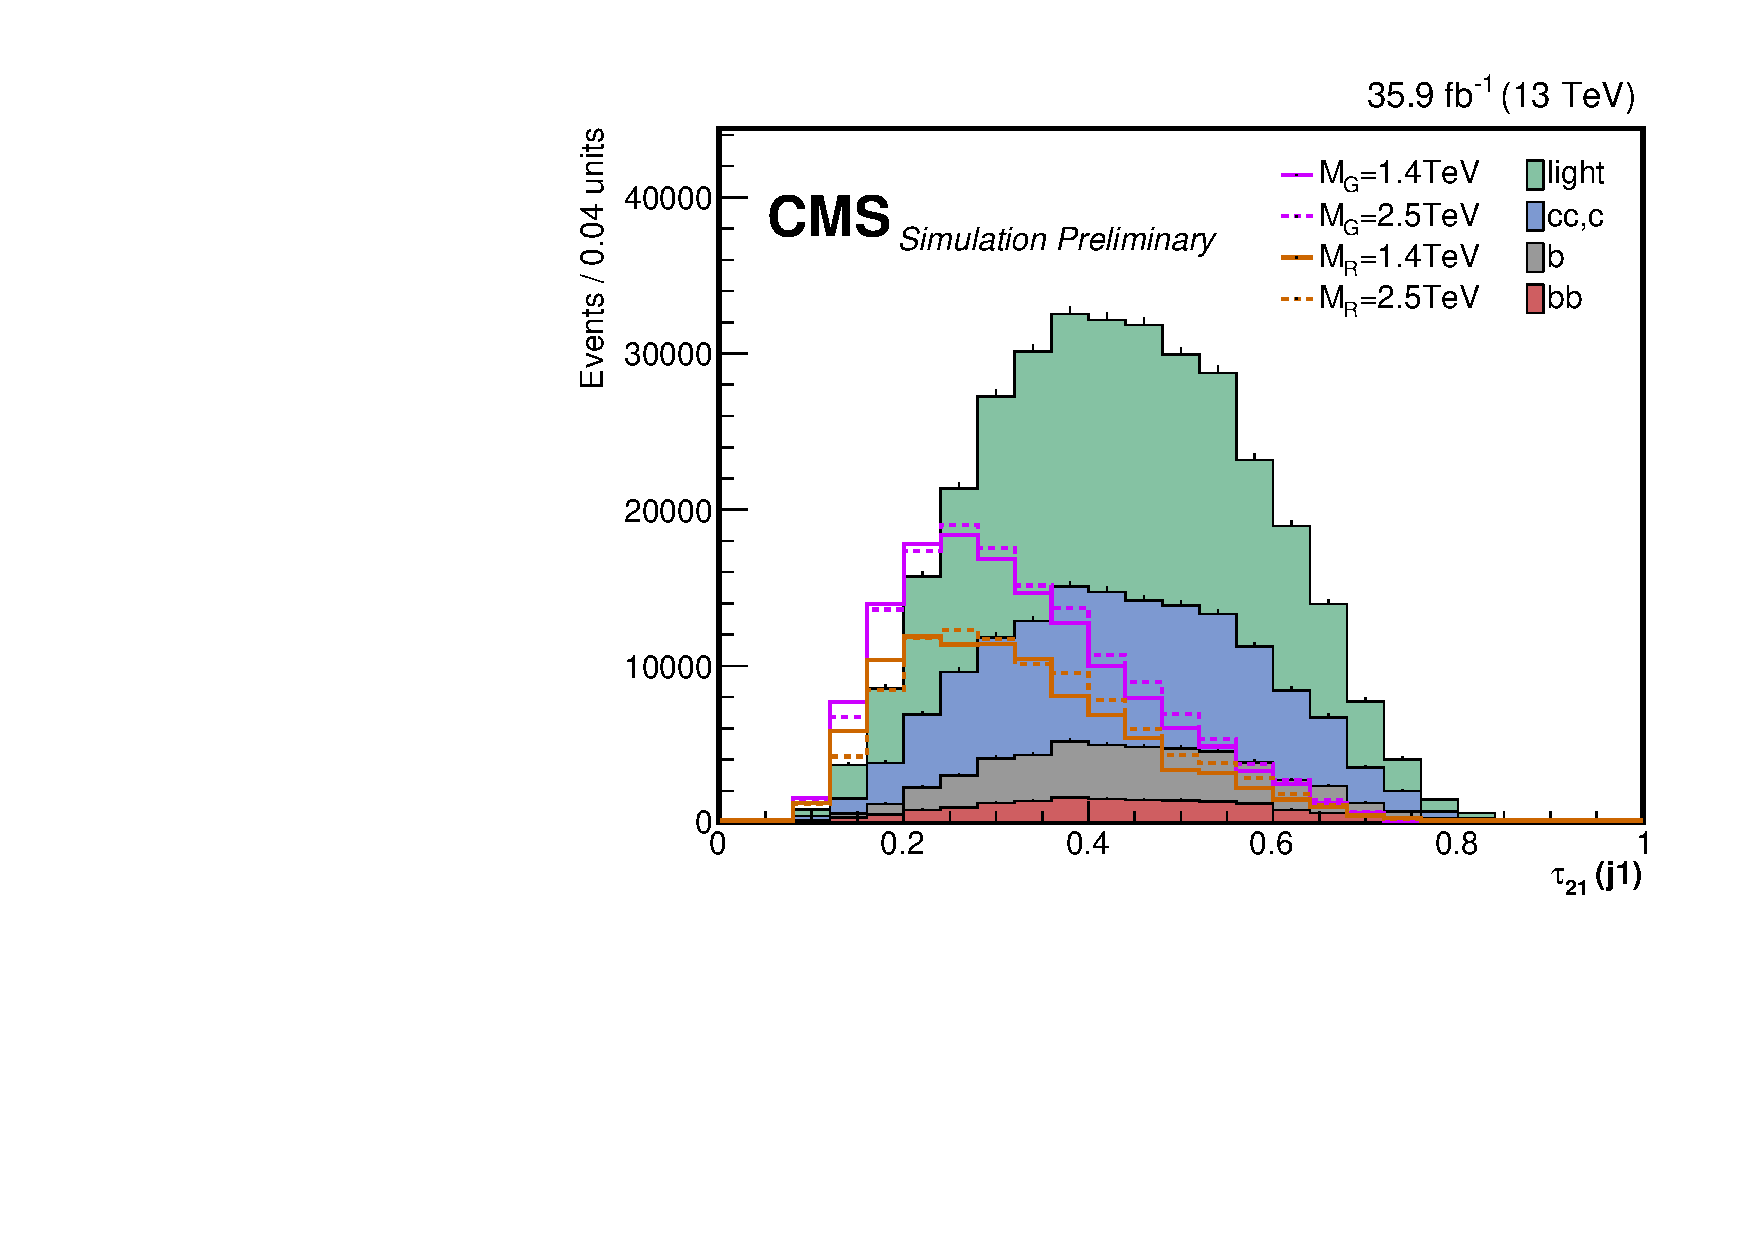
\includegraphics[width=0.5\textwidth]{Figures/MC_N1/puppiTau21_j0.pdf} &
%    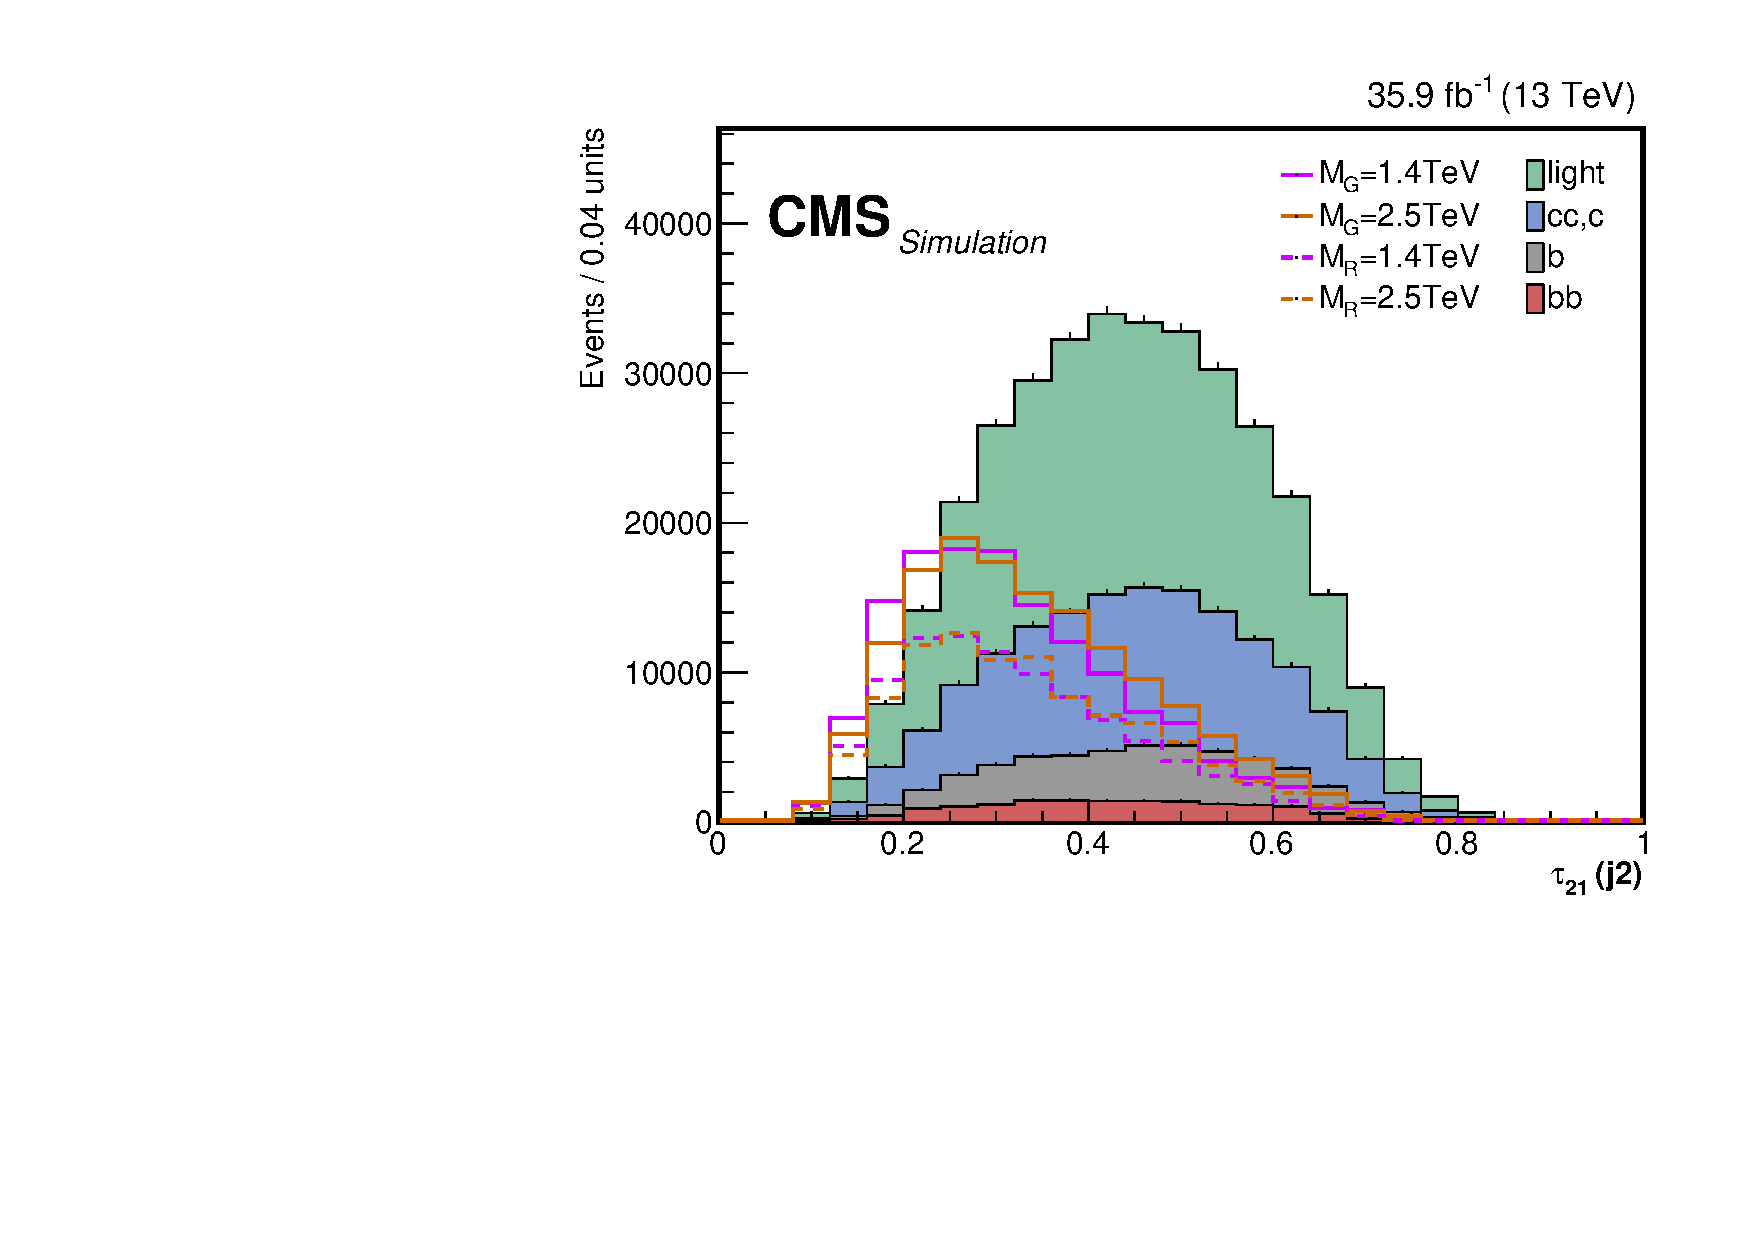
\includegraphics[width=0.5\textwidth]{Figures/MC_N1/puppiTau21_j1.pdf} \\
%     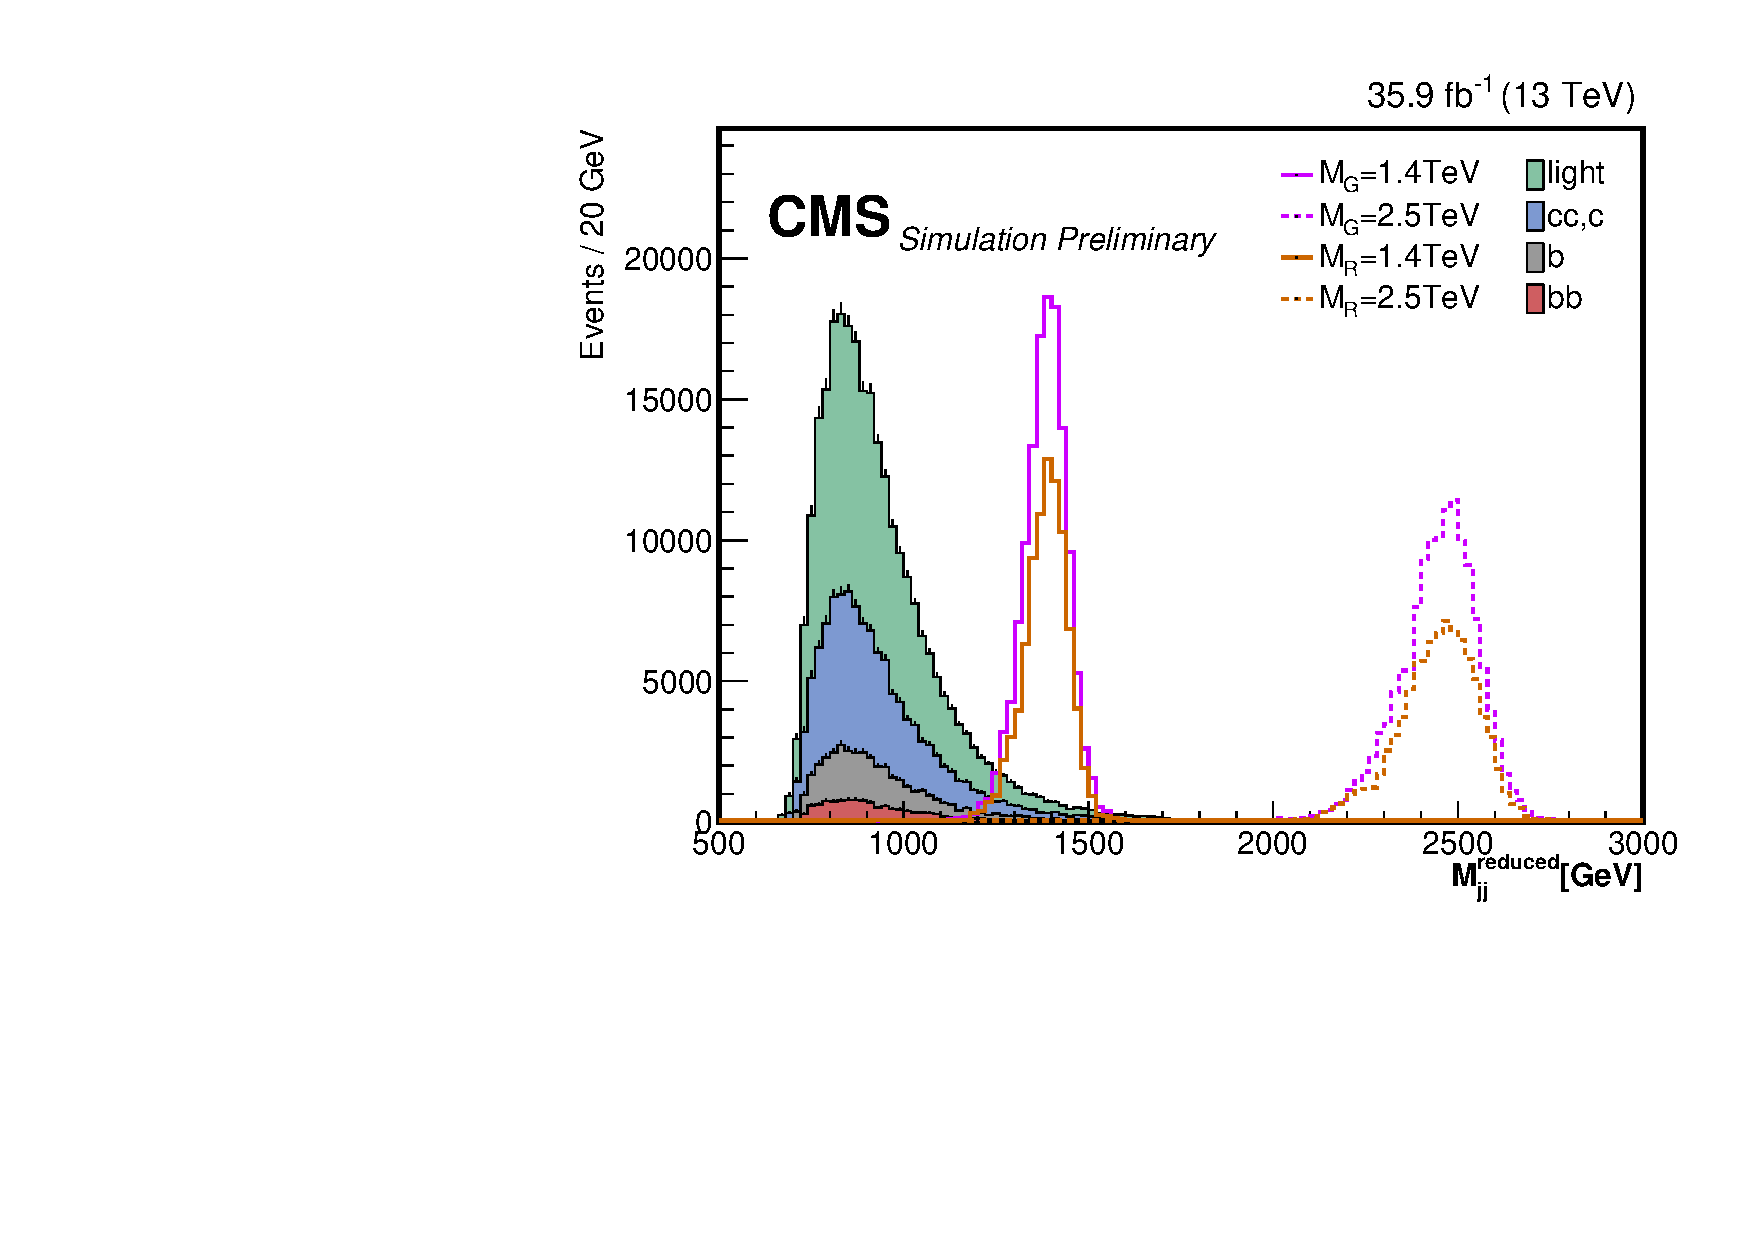
\includegraphics[width=0.5\textwidth]{Figures/MC_N1/totalMassRed.pdf} &
%    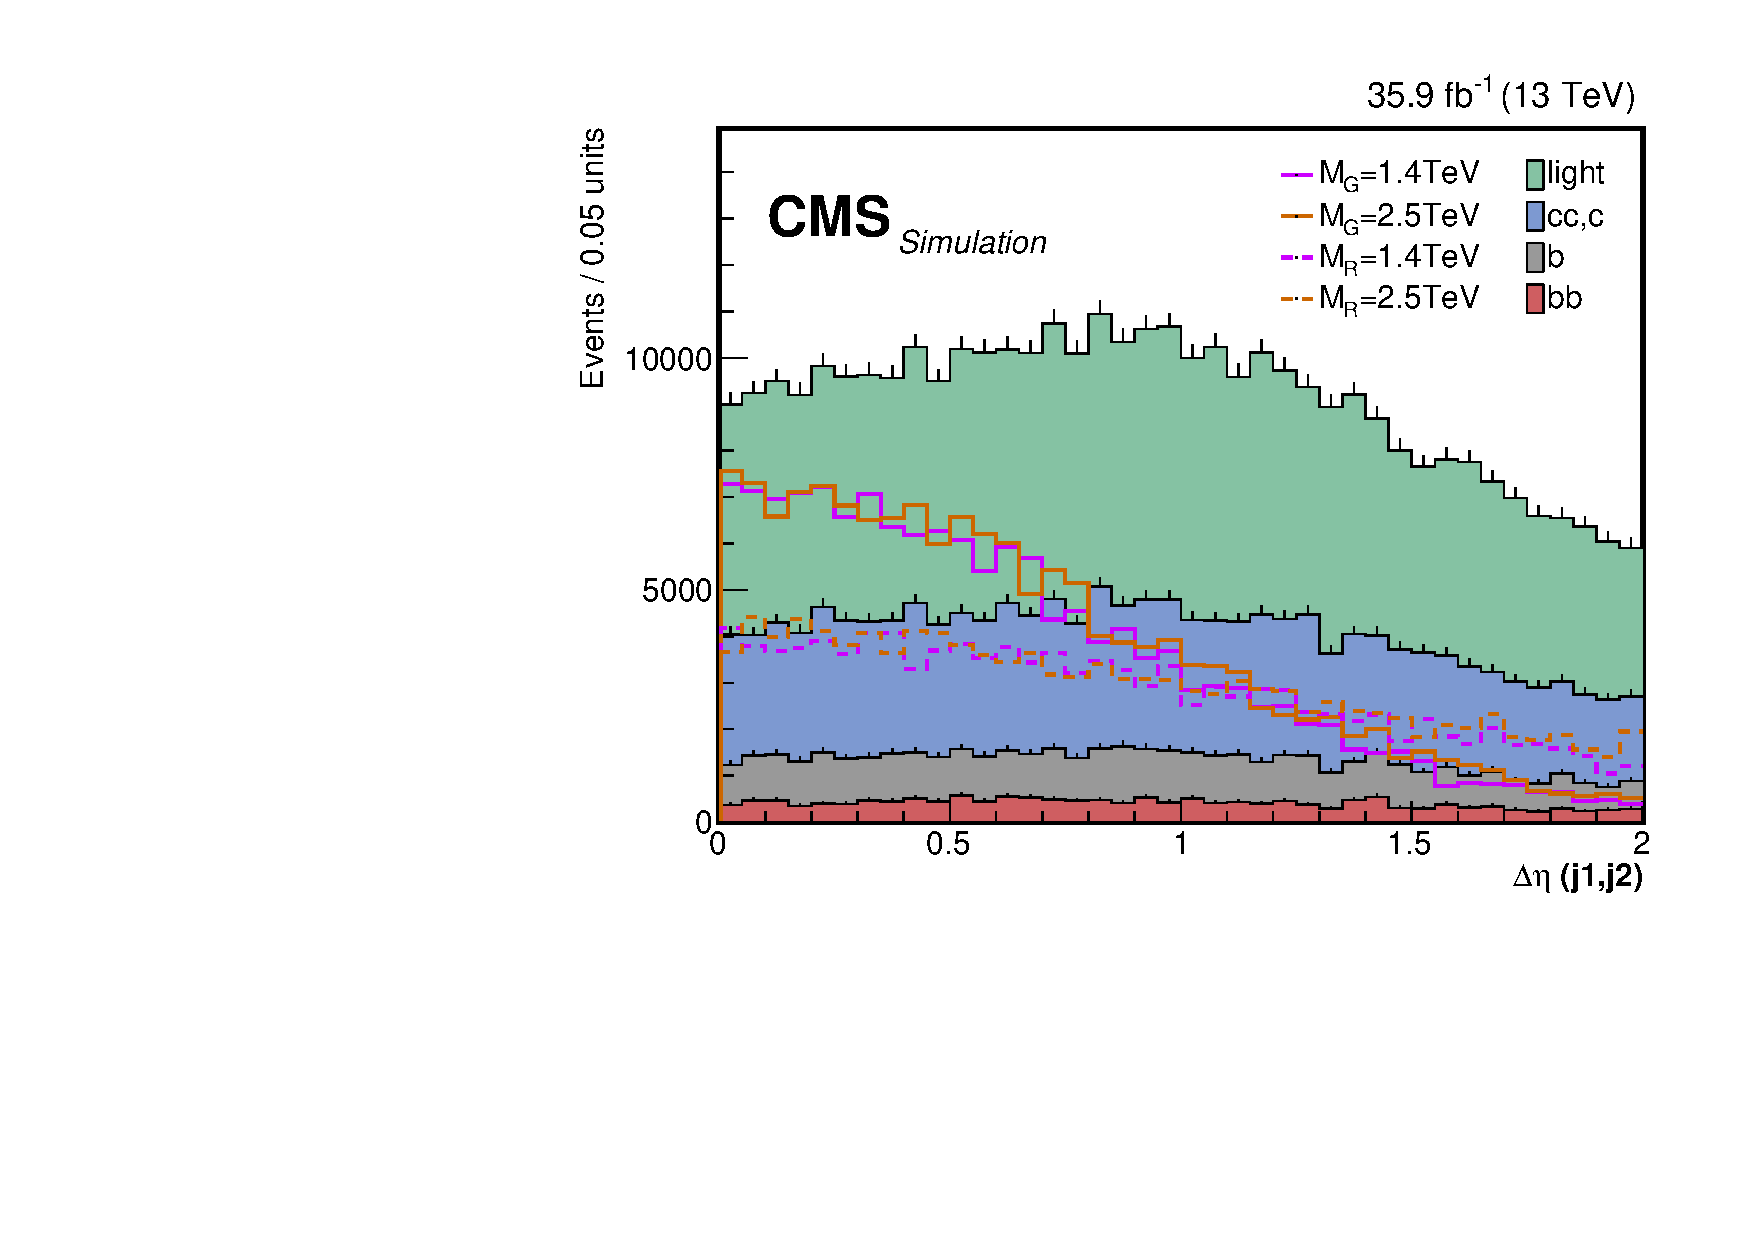
\includegraphics[width=0.5\textwidth]{Figures/MC_N1/deltaEta.pdf} \\
%  \end{tabular}
%  \caption{The comparison of signal and background. The signals of $M_{X}$ = 1.4 TeV and 2.5 TeV from both models are shown. The cross section is set to 20 pb in the figures. Multi-jet events are seperated into four categories summarized in the table 2.10. From top to buttom are the comparison of PUPPI soft-drop mass, $\tau _{21}$ of leading (left) and next leading (right) AK8 jet, the reduced mass (buttom left), and |$\Delta \eta $ (the two leading AK8 jets)| (buttom right).}
%  \label{fig:hvt_brs}
%\end{figure}
  % Chapter Detector 

\chapter{Collider and Detector} \label{chap:2}
%http://iopscience.iop.org/article/10.1088/1748-0221/3/08/S08004/pdf

\section{Large Hadron Collider}%P29
Large Hadron Collider (LHC) is located at Geneva region about 100 meters underground, built and operated by European Organization for Nuclear Research, CERN. 
Its circumference is 27-km-long, and two proton beams in which the energy of each proton is 6.5 TeV produce collisions at center-of-mass energy reaching 13 TeV in 2015. 
LHC is the largest collider in the world, both in size and in center-of-mass energy.
Besides, LHC also provides heavy-ion collision to include the study of the behavior of quantum chromo dynamics, QCD, under high-density parton momentum fraction and the study of the properties of gluon-quark plasma, which is thought to constitute the universe for few $\mu$s after the Bing Bang~\citep{Heavyions}. 
When it operates, the intervals between proton bunch crossing is 25 ns, that is to say,  4 $\times 10^7$ events are produced per second. 
Besides, an average of 20 inelastic collisions will be produced in a single bunch crossing.
It is undoubtedly a challenging requirement on technique not only to reduce the number of events recorded by triggers but also to alleviate the effect by inelastic collision that cause pile-ups.

\section{The Compact Muon Solenoid Detector}

As one of the detectors of the LHC, the Compact Muon Solenoid Detector, CMS~\citep{CMSDetector}, shares the same aims of the LHC.
Basically, it will elucidate the physical properties of the Higgs boson whose mass is around 125 GeV, and it will also test the mathematical consistency of Standard Model, SM, at TeV scale.
People also hope to find new physic beyond SM where Supersymmetry and Extra Dimension is often being considered. The latter necessitates the finding of graviton in TeV scale.
All researches need a delicate design of a detector, including good charged particle reconstruction to trace the vertex, good EM energy resolution, and good measurement of missing transverse momentum and mass resolution.
\begin{itemize}
\item The tracker: The high granularity tracker at inner detector can well reconstruct the trace of charged particles. It is also indispensable for identifying b-flavored jets and $\tau$.  
\item The muon chamber: The muon chamber combined with tracker information under the magnetic field of opposite direction can  interpolate together to reduce mismatching rate in muon reconstruction, to enhance precision of measurement on high transverse momentum muons, and to identify the cosmic muons from outside of the detector.
\item The calorimeters: The calorimeters facilitate the shower and measure the energy of post-shower particles. The information will further be clustered into the energy corresponding to their mother particles.
\end{itemize}

\begin{figure}[t]
  \begin{center}

    \includegraphics[width=0.5\textwidth]{Figures/cms_160312_02.pdf} 
    \end{center}
  \caption{The three-dimension sketch-up image of the CMS detector~\citep{CMSImage}.}
\end{figure}

\subsection{Detector Kinematics} 
To better describe the geometry of the detector, a set of convention is adopted. The z axis is along the beam line, and the positive direction points to the proton beam moving in the counter-clockwise direction. The x axis points to the center of the LHC circle. The xy plane is perpendicular to z axis and can be described by $\phi $:
\begin{equation} \label{eq1}
\begin{split}
x=rcos\phi, y=rsin\phi,
\end{split}
\end{equation}
where $\phi$ is the azimuthal angle, r is the distance from the z axis on xy plane. The variable rapidity y is related to the angle $\theta$ between one momentum vector and the z axis. The difference of rapidity is invariant under boosts along the z axis. When particles travel near the speed of light, its mass is negligible. Hence, $E$ $\thickapprox$ $|\vec{p}|$ and rapidity could be approximated by pseudo rapidity $\eta$ $\thickapprox$ y, while $E$ = $|\vec{p}|$ for a massless particle.
\begin{equation} \label{eq1}
\begin{split}
y = \frac{1}{2} ln( \frac{E+p_z}{E-p_z} ), \eta = \frac{1}{2} ln( \frac{|\vec{p}|+p_z}{|\vec{p}|-p_z} ) = -log[tan(\theta /2)]
\end{split}
\end{equation}

\subsection{Magnet System} 
In order to have a good resolution for charged particles in the trackers, magnetic field must maintain to bend the tracks of charged particles. 
Providing the magnetic field of CMS, the superconducting solenoid is installed between the calorimeters and muon chambers with a diameter of 6.3 m, length of 12.5 m, and mass of 200 t. 
Designed to have 3.8 T magnetic field at the center of the detector along positive z direction, the solenoid uses four layers based on the Ampere-turn (41.7MA-turn) and made of aluminum alloy.
The width of one layer is far less than its counterpart of other detectors, and its lower limit is restricted by the magnetic pressure and the material property of aluminum.
It also breaks the convention, for that the magnetic stress is shared between itself and the outer mandrels. 
The yoke whose proposes are guiding the magnetic field and absorbing particles except muons and neutrinos is composed of five barrel wheels and 6 endcap disks~\citep{yoke}. 
Besides, to avoid the "quench back" effect, where the eddy currents induced in outer mandrels heat up the coil above superconducting critical temperature, 
a protecting circuit is designed and worked by either fast discharge or slow discharge through dumping. 

\subsection{Tracker Detector} 
Having precisely-reconstructed primary and secondary vertices, the Tracker detector is designed to be at innermost part of the CMS detector.
It needs to be fast enough to collect data between 25 ns interval of bunch crossing and high granularity enough to identify the trajectories. 
Two kinds of tracker detector are used for different purposes, the pixel trackers and the strip trackers. 
While the former is better at determining three dimensional space and at enduring the radiation dose, 
the latter covers larger total area since it costs less per area. 
There are three cylindrical pixel detectors at radii of 4.4, 7.3 and 10.2 cm and two disks of pixel detectors at |z| of 34.5 and 46.5 cm on each side of the interaction point. 
They together give coverage to pseudo rapidity |$\eta $| $<$ 2.5 and an area of about 1 $m^2$ with total 66 million pixels whose size is 100 $\times$ 150 $\mu m^2$ each. 
The strip detectors are separated into several subsystems. The Tracker Inner Barrel and the Tracker Inner Disk (TIB/TID) at radii extending to 55 cm together, composing 4 layers and 3 disk on each side, 
provide four $r-\phi $ measurements with resolution of 23 $\mu m$ and of 35 $\mu m$ by the first two layers and the others respectively. 
Tracker Outer Barrel (TOB) ranges toward radius of 116 cm and performs six $r-\phi $ measurements with resolution of 53 $\mu m$ and of 35 $\mu m$ by the first four layers and the others respectively.
In addition, Tracker EndCap (TEC) gives another 9 measurements on $\phi $ by its nine layers installed at 124 cm $<$ |z| $<$ 282 cm.
 
\subsubsection{Pixel Trackers}
%https://twiki.cern.ch/twiki/pub/Main/UndergradElog2014/pixelDetectors.pdf
The pixel trackers constitutes of pn-junctions operated in depletion. 
When particles pass depletion zone, induced electron-hole pairs will produce signal current and further be amplified and read out. 
To take the high-density radiation dose into account, a n$^+$-doped electrodes in n-doped substratrate design is chosen as sensor. 
Another advantage of the n-on-n concept is that a guard ring can be made around the sensor to prevent voltage breakdown in air (1.2V/$\mu $m). 
The isolation between electrodes prevents electrodes from shortening after radiation. Open p-stop and moderate p-spray are isolation designs implemented on disks and barrel respectively~\citep{PixelD}.

\subsubsection{Strip Trackers}
The elements in the trackers are single-sided p-on-n silicon micro-strip sensors. 
Besides, the six-inch wafers are used instead of four-inch wafers to reduce the cost. 
As the built-on surface charge of $\langle$100$\rangle$ crystal orientation of n substratrate is smaller than $\langle$111$\rangle$ one, 
the $\langle$100$\rangle$ is chosen to maintain the capacitance after irradiation. The $\langle$xyz$\rangle$ is the sign used in solid state physics, which represents the direction of the plane of a crystal. To clarify, $\langle$100$\rangle$ means the first plane intercepting the x, y, and z-axis at 1, 0, and 0 respectively. Other planes are perpendicular to this plane and have distance by $\sqrt{1^2+0^2+0^2} \times$ n. Following the same rule, the first plane in $\langle$111$\rangle$ crystal intercepts the x, y, and z-axis at 1, 1, and 1 respectively. Other planes are perpendicular to this plane and have distance by $\sqrt{1^2+1^2+1^2} \times$ n.

\subsection{Electromagnetic Calorimeter} 
%118
The electromagnetic calorimeters, ECAL, is used to measure the energy of electromagnetic, EM, particles through EM shower. 
In other words, they can reconstruct the mother particles of electrons and photons indirectly.
The system is composed of the ECAL Barrel (EB) in |$\eta $| $<$ 1.479 and the ECAL Endcap (EE) in 1.479 $<$ |$\eta $| $<$ 3.0. 
Lead-tungstate crystals (PbWO4) are chosen as scintillator where shower is collected and as the material to induce shower.
Its short Radiation length (0.89cm) and Moliere radius (2.2cm) are appropriate for compact space in CMS.
The photon detectors are set on the back on each crystal. 
Avalanche photodiodes are used for EB, while vacuum phototriodes are used for EE. 
Besides, the preshower detector (ES) is installed in front of the EE where 1.653 $<$ |$\eta $| $<$ 2.6. 
There are two layers: lead radiators and silicon strip sensor.
The ES is mainly used to identify $\pi ^0$ and assists the identification of electrons against minimum ionizing particles.
 

\subsection{Hadron Calorimeter} 
The hadron calorimeters measure the energy of hadrons, and they are substantial to detect the neutrinos or exotic particles by measuring missing transverse momentum.
There are four subsystems including the barrel (HB) , the endcap (HE) , the outer (HO) , and the forward (HF) designs.
Both the HB and the HE are sampling calorimeters. 
The HB covers |$\eta $| $<$ 1.3, while the HE covers 1.3 $<$ |$\eta $| $<$ 3.
They are both consisted of scintillators interleaved with C26000 cartridge brass (70$\% $ copper and 30$\% $ zinc) absorbers because of high density of brass.
Six brass layers of 50.5 mm each, eight brass layers of 56.5 mm each along with front and back plate of 40 and 75 mm give totally 87cm thickness of absorbers in barrel, while the thickness of absorbers in endcap is 79mm for each layer.
The HB is not thick enough to contain all the energy of high-energy particles.
Thus, the HO is installed outside the HB to catch the rest of the later showers combined with the HB to give about 11.8 interaction lengths in total. Outside the solenoid, five iron rings haing width of 2.536m each along z-axis together form the return yoke. The first layer of each iron ring has one HO layer installed at the outer side, while two layers are installed on inner and outer sides of the central ring (Ring0) because of its shortest radical distance shown in Fig.~\ref{fig:22}. Each module includes 10 mm scintillator whose material is Bicron BC408.
In addition, to detect the very forward jets thus to improve the measurements of missing transverse momentum, the HF is needed whose coverage extends to about |$\eta $| $=$ 5.
As the energy deposit is not uniformly distributed in the detector, the forward region takes higher radiation dose.
The HF must be most radiation-hard by means of the shielding including 40 cm steel, 40 cm concrete, and 5cm of polyethylene. With the same reason, the quartz fibers (fused-silica core and polymer hard-cladding) is chosen as the absorber material.

\begin{figure}[t]
  \begin{center}

    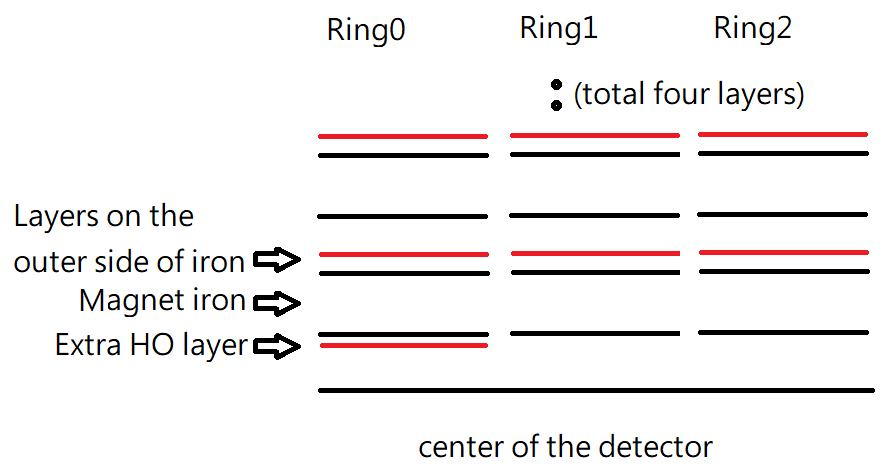
\includegraphics[width=0.5\textwidth]{Figures/20289635_1397863916957915_543326343_n.png} 
    \end{center}
  \caption{The layout of the HO rings in z-r direction.}
  \label{fig:22}
\end{figure}

\subsection{Muon Detector} 
Muon identification ensures the rate of the expected background is well measured. 
For example, backgrounds whose final state includes at least one Z boson decaying into di-muons. 
This is essential for the discovery of Higgs mechanism where background of ZZ is dominant.
Besides, some physics beyond Standard Model, Supersymmertry for example, has muons in its final state.
The CMS muon system is made up of three kinds of gaseous chamber detectors. 
First, the barrel drift tube (DT) chambers contain four layers distributing between |$\eta $| $<$1.2.
The first three layers include totally 12 chambers, eight for $r-\phi$ measurements and four for |z| measurements, while the last layer only measures $r-\phi$. 
With a width of single cell of 42 mm, the maximum drift distance is its half, which has 380 ns maximum drift time. 
The electric field in the cells filled with 85$\% $ Ar and 15$\% $ CO$_2$ is set up by 3600V anode wire at the central, 1800V two electrode strips at the ceil and the floor, and two  1800V cathode strips on each side. 
Second, the cathode strip chambers (CSC) have 6 layers and are grouped into 4 stations.
Their fast response is suitable for more non-uniform magnetic field, since more muons pass through in forward region, the CSC chambers are placed at 0.9 $<$ |$\eta $| $<$ 2.4.
The CSC disks are separated into strips by either 20$^{\circ} $ or 10$^{\circ} $ in $\phi $. 
Each chamber has 6 gas gaps with anode wires separated by 7 cathode panels. 
The cylindrical wires make the r-coordinate measurements, while the charges induced on the strips interpolate to determine $\phi $ coordinate.
The gas mixture is 40$\% $ Ar + 50$\% $ CO$_2$ +10$\% $ CF$_4$. 
Last, the resistive plate chambers (RPC) with fast response are added to muon system to complement the time resolution, especially with multiple-muon events.
However, they have to work with DT and CSC, for RPC has worse spatial resolution than the others.
There are two layers in each station for the first two stations of DT and one layer in each station for the other two stations. 
In addition, three disks in the first three CSC to improve the time resolution are used in determination of time of bunch crossing and muon $p_T$ reconstruction.
A module consists of 2 gaps in which there is a gas plate held by two bakelites, referred as the up gap and the down gap with a strip between them connecting to the read-out .
The triggers in muon system using RPC information can perform at high rate and a rather high $p_{T}$ of muons threshold.

\section{The trigger system}
The interval between bunch crossing in LHC is 25 ns which corresponds to a rate of events of 40 MHz.
The trigger system is required to reduce the rate of events for recording on tape.
The system includes Level-1 Trigger system (L1) and High-Level Trigger (HLT) together.
The L1 Trigger will reduce at least to 100 kHz, and the HLT will then reduce to a maximum of 30kHz.
The L1 Trigger is made up of several hardware programmable electronics which collect information from muon system and calorimeters.
On the other hand, the HLT triggers are software-like triggers which have the access to complete readout of data. 
Thus, they are able to do the complex calculation similar to those done in the analysis off-line. 
The algorithm of HLT will be improved through the time, so it will not be detailed here.
 
	% Chapter Analysis Strategy

\chapter{Analysis Strategy} \label{Analysis Strategy}

The target of the analysis is to search for the heavy resonances decaying to di-Higgs where mass of heavy resonances is above 800 GeV. Each Higgs boson is assumed to further decay to ${b\bar{b}}$ and is reconstructed in a boosted jet including two b-flavored-like sub-jets by anti-kT08 algorithm. Higgs identification is done by selection on PUPPI soft-drop mass, N-subjetness, and double b-tagger. 

\hypersetup{colorlinks,linkcolor=black,urlcolor=black}
\section{Data and Simulated Samples} \label{Data and simulated samples}
The analysis is preformed based on the data collected in pp collision with the CMS detector at $\sqrt{s}$ = 13 TeV. The integrated luminosity is 35.9$fb^{-1}$. Runs in which the detector normally operates was chosen according to the golden JSON file: $\href{https://cms-service-dqm.web.cern.ch/cms-service-dqm/CAF/certification/Collisions16/13TeV/ReReco/Final/Cert_271036-284044_13TeV_23Sep2016ReReco_Collisions16_JSON.txt}{Cert\_271036-284044\_13TeV\_23Sep2016ReReco\_Collisions16\_JSON.txt}$. The samples of data are listed in table 3.1. %to-do # table

\begin{table}[h!]
  \begin{center}
    \begin{tabular}{l|l|l}
    Dataset & Processing & Int. lumi. ($fb^{-1}$) \\
    \hline
    JetHT/Run2016B & 23Sep2016 & 5.9\\
    JetHT/Run2016C & 23Sep2016 & 2.6\\
    JetHT/Run2016D & 23Sep2016 & 4.4\\
    JetHT/Run2016E & 23Sep2016 & 4.1\\
    JetHT/Run2016F & 23Sep2016 & 3.2\\
    JetHT/Run2016G & 23Sep2016 & 7.7\\
    JetHT/Run2016H & PromptReco & 8.9\\
    \hline
    Total & & 35.9\\
    \end{tabular}
  \end{center}

  \caption{List of datasets used in the analysis and its corresponding integrated luminosity in pp collision at $\sqrt{s}$ = 13 TeV.}
\end{table} 

\section{Monte Carlo Simulation} \label{Monte Carlo Simulation}	
The Monte Carlo, MC, simulations in the analysis are bulk graviton, radion, and multijet events. MadGraph is used to produce the simulated particles and their decay\citep{Alwall2011}. Bulk graviton, radion are used for setting the upper limit of cross section, while multijets events are used for testing the background estimation method and not used for final results. The names and the number of events of samples are listed in the table 3.2-3.4. The cross section of signal used in the final results are listed in the table 3.5\citep{WED_BG_13TeV,WED_radion_13TeV,WED_BGHHDecay_13TeV,WED_radionHHDecay_13TeV}. Since the distributions of pile-ups of data and of MC are different, a pile-up re-weighting is applied to MC samples. Here the distribution of pile-ups of data is derived by using minibias cross section of pp collision of 69.2 mb\citep{Aaboud:2016mmw}.%to-do 
%https://journals.aps.org/prl/abstract/10.1103/PhysRevLett.117.182002
%https://link.springer.com/article/10.1007%2FJHEP06%282011%29128
\begin{table}[h!]
  \begin{center}
    \begin{tabular}{l|l|l}
    Samples & $\sigma$(pb) & Events \\
    \hline
    BulkGravTohhTohbbhbb$\_$narrow$\_$M-1000$\_$13TeV-madgraph & 2.66 & 50000 \\
    BulkGravTohhTohbbhbb$\_$narrow$\_$M-1200$\_$13TeV-madgraph & 0.95 & 50000 \\
    BulkGravTohhTohbbhbb$\_$narrow$\_$M-1400$\_$13TeV-madgraph & 0.37 & 50000 \\
    BulkGravTohhTohbbhbb$\_$narrow$\_$M-1600$\_$13TeV-madgraph & 0.18 & 50000 \\
    BulkGravTohhTohbbhbb$\_$narrow$\_$M-1800$\_$13TeV-madgraph & 0.084 & 48400 \\
    BulkGravTohhTohbbhbb$\_$narrow$\_$M-2000$\_$13TeV-madgraph & 0.041 & 50000 \\
    BulkGravTohhTohbbhbb$\_$narrow$\_$M-2500$\_$13TeV-madgraph & 0.007 & 50000 \\
    BulkGravTohhTohbbhbb$\_$narrow$\_$M-3000$\_$13TeV-madgraph & 0.0017 & 50000 \\
    	\hline
    \end{tabular}
  \end{center}

  \caption{List of bulk graviton $\rightarrow$ HH $\rightarrow$ $b\bar{b}$ Monte Carlo simulation and its corresponding cross section and the number of events. The cross sections are used in McM process at leading order, LO, and not used in the final results.}
\end{table} 

\begin{table}[h!]
  \begin{center}
    \begin{tabular}{l|l|l}
    Samples & $\sigma$(pb) & Events \\
    \hline
    RadionTohhTohbbhbb$\_$narrow$\_$M-1000$\_$13TeV-madgraph & 1318 & 50000 \\
    RadionTohhTohbbhbb$\_$narrow$\_$M-1200$\_$13TeV-madgraph & 116.2 & 50000 \\
    RadionTohhTohbbhbb$\_$narrow$\_$M-1400$\_$13TeV-madgraph & 67.97 & 50000 \\
    RadionTohhTohbbhbb$\_$narrow$\_$M-1600$\_$13TeV-madgraph & 41.74 & 50000 \\
    RadionTohhTohbbhbb$\_$narrow$\_$M-1800$\_$13TeV-madgraph & 26.57 & 50000 \\
    RadionTohhTohbbhbb$\_$narrow$\_$M-2000$\_$13TeV-madgraph & 17.43 & 50000 \\
    RadionTohhTohbbhbb$\_$narrow$\_$M-2500$\_$13TeV-madgraph & 6.646 & 50000 \\
    RadionTohhTohbbhbb$\_$narrow$\_$M-3000$\_$13TeV-madgraph & 1.519 & 50000 \\
   \hline
    \end{tabular}
  \end{center}
  \caption{List of radion $\rightarrow$ HH $\rightarrow b\bar{b} $ Monte Carlo simulation and its corresponding cross section and the number of events. The cross sections are used in McM process at LO and not used in the final results.}
\end{table} 

\begin{table}[h!]
  \begin{center}
    \begin{tabular}{l|l|l}
    Samples & $\sigma$(pb) & Events \\
    \hline
    QCD$\_$HT-100to200  & 2.785 $\times$ 10$^7$ & 81,906,377 \\
    QCD$\_$HT-200to300  & 1.717 $\times$ 10$^6$ & 18,752,566 \\
    QCD$\_$HT-300to500  & 3.513 $\times$ 10$^5$ & 20,312,907 \\
    QCD$\_$HT-500to700  & 3.163 $\times$ 10$^4$ & 19,755,616 \\
    QCD$\_$HT-700to1000  & 6831 & 15,595,234 \\
    QCD$\_$HT-1000to1500  & 1207 & 4,966,123 \\
    QCD$\_$HT-1500to2000  & 119.9 & 3,964,488 \\
    QCD$\_$HT-2000toInf  & 25.24 & 1,984,407 \\
	\hline
    \end{tabular}
  \end{center}

  \caption{List of multijet Monte Carlo simulation and its corresponding cross section and the number of events. The cross sections are used in McM process at LO.}
\end{table}

%https://github.com/CrossSectionsLHC/WED/blob/master/KKGraviton_Bulk/GF_NLO_13TeV_ktilda_0p1.txt
%https://github.com/CrossSectionsLHC/WED/blob/master/Radion_Bulk/GF_NLO_13TeV_LR_3TeV_kl_35.txt
%https://github.com/CrossSectionsLHC/WED/blob/master/KKGraviton_Bulk/Decay_long.txt
%https://github.com/CrossSectionsLHC/WED/blob/master/Radion_Bulk/Decay_long_kl_35_arxiv1110.6452.txt

\begin{table}[h!]
  \begin{center}
    \begin{tabular}{l|l|l}
    M$_{X}$(GeV) &  $\sigma$(pp$\rightarrow$X$_{G}\rightarrow $HH) (fb)& $\sigma$(pp$\rightarrow$X$_{R}\rightarrow $HH) (fb)\\
    \hline
    750 & 2.408 & 155.46 \\
    800 & 1.771 & 128.68 \\
    900 & 0.953 & 88.433\\
    1000 & 0.559 & 62.057\\
    1500 & 0.057 & 12.897\\
    1800 & 0.018 & 5.6664\\
    2000 & 9.03E-03 & 3.3868\\
    2500 & 1.86E-03 & 1.0193\\
    3000 & 3.03E-04 & 0.3280\\
    3500 & 1.15E-04 & 0.1114\\
    4500 & 8.91E-06 & 1.26E-02\\
	\hline
    \end{tabular}
  \end{center}

  \caption{List of the cross section $\times$ the branch ration of HH decay in fb. The model $k/\bar{M_{Pl}}$ = 0.1 in bulk graviton is considered, and the model $	\Lambda _R$ = 3TeV and $kl$ = 35 of radion is considered.}
\end{table}



\section{Event Reconstruction and Selection} \label{Event reconstruction and selection}
%MET Filters & AND \\
%https://twiki.cern.ch/twiki/bin/view/CMS/MissingETOptionalFiltersRun2#How_to_run_the_Bad_Charged_Hadro 
To reduce the impact from both cosmic particles and noise of calorimeters, missing transverse energy, MET, filters are applied.
If all particles are detected and well-reconstructed in the detector, the sum of transverse momentum will be zero. However, if there are noise, ill-reconstructed particles or jets, the sum of transverse momentum will not equal to zero, and the negative of its value is defined as MET.  
The filters remove most events having anomaly MET based on different information given from the detectors. We require the event to pass all filters listed in table 3.6\citep{MissingETOptionalFiltersRun2}.  %table 
\begin{table}[h!]
  \begin{center}
    \begin{tabular}{l}
    Triggers \\
    \hline
    primary vertex filter\\
    beam halo filter\\
    HBHE noise filter\\
    HBHE iso noise filter\\
    ECAL TP filter\\
    ee badSC noise filter\\
	Bad PF Muon Filter\\
	Bad Charged Hadron Filter\\ 
    \hline
    \end{tabular}
  \end{center}

  \caption{List of MET filters applied in the analysis.}
\end{table}

%Number of good vertex & $>$1 \\
After passing MET filters, at least one reconstructed pp collision vertex which passes following criteria is required in an event.
\begin{itemize}[noitemsep]
\item Number of degree of freedom $>$ 4
\item Absolute displacement from the beamspot position along the z direction $<$ 24 cm
\item Absolute displacement from the beamspot position along the transverse direction $<$ 2 cm
\end{itemize}


%Lepton veto & one tight-tagged or two opposite charged loose-tagged \\
For the final state is all-hadronic, lepton veto is implemented. The event will be vetoed either if there is a tight-tagged muon or electron, or if there are two loose-tagged mouns or electrons with opposite charged.

\subsection{Higgs Jet Reconstruction} 
%http://iopscience.iop.org/article/10.1088/1126-6708/2008/04/063/pdf
%http://cds.cern.ch/record/1194487
%http://cds.cern.ch/record/1247373
Each candidate of particles is reconstructed with Particle-Flow, PF, algorithm in CMS by all the detector components\citep{CMS-PAS-PFT-10-001,PFPAS2009}. In the algorithm, priority of reconstruction form high to low are: muons, electrons, photons, charged hadrons, and neutral hadrons.

The jets are clustered with anti-$k_{T}$ algorithm by PF candidates\citep{antiKtAlgorithm}. Anti-$k_{T}$ algorithm is done described below: 
\begin{equation} \label{eq1}
\begin{split}
d_{ij} = min(k^{2p}_{ti},k^{2p}_{tj})\dfrac{\Delta ^2_{ij}}{R^2}\\
d_{iB} = k^{2p}_{ti}, 	
\end{split}
\end{equation}
where $\Delta ^{2}_{ij}= (y_{i}-y_{j})^2+(\phi_{i}-\phi_{j})^2$, and $k_{ti}$, $y_{i}$, and $\phi _{i}$ are the transverse momentum, rapidity, and azimuth of particle i. The value of p is set according to the algorithm. The anti-$k_{T}$ algorithm uses p = -1. 
Considering minimum term of $k^{2p}_{t}$ between one hard particle and the selected soft particle compared to that between the soft particle and another soft particle, the former will be smaller because while the transverse momentum of hard particles is larger, its inverse square is smaller. 
Therefore, $d_{ij}$ of the former is shorter, that is, a soft particle is more likely to cluster with hard particle around it. 
As a consequence, if there is no other hard particle within the range 2R of a hard particle, it will cluster a conical jet with all soft particles within range R. 
In other situation where the distance of two hard particles is between R and 2R, one can show that the particle having larger transverse momentum will cluster a  conical jet, while the other is partly conical.
Last, where distance of two hard particles $<$ R, two particles will merge into single jet. In the analysis, the jets is clustered using anti-$k_{T}$ with range parameter R set to 0.8 (refrred as AK8 jets).

%https://arxiv.org/pdf/1407.6013.pdf
In one bunch crossing, the vetex having highest energy called primary vertex, and the others are called pile-ups, PUs. PUs may contribute some components in jet clustering which do not origninally belong to them. We can mitigate the effect by PUPPI algorithm\citep{puppi}, which is described below:
First, a shape $\alpha _{i}$ of a particle i is defined: 
\begin{equation} \label{eq2}
\begin{split}
\alpha_i = log \sum\limits_{j\in event} \xi _{ij} \times \Theta(\Delta R_{ij} - R_{min}) \times \Theta(R_0 - \Delta R_{ij}) \\
\xi _{ij} = \dfrac{p_{Tj}}{\Delta R_{ij}}, 
\end{split}
\end{equation}
where $\Theta$ is the Heaviside step function, $p_{T}$ is the transverse momentum, and $\Delta R_{ij}$ is the distance between particle i and j in $\eta \phi$ space. Hence, only particles falling in the cone size $R_0$ but not closer than $R_{min}$ contribute to $\alpha $. $R_0$ represent the locality of a jet, and $R_{min}$ is most restricted by resolution of the detector. Then we seperate events into two cases: with and without tracker information. The former is used to weight the charged particles in central region, while the latter is used for charged particles in forward region and neutral particles. An addition scale factor depending on rapidity is applied to forward region. The calculation of weight uses the quantities of the median and the left-side RMS of $\alpha $ distribution. Finally, the weight of a particle is: 
\begin{equation} \label{eq3}
\begin{split}
\chi ^2_{i} = \Theta(\alpha _i - \bar{\alpha } _{PU}) \frac{ ( \alpha _i - \bar{\alpha } _{PU})^2 }{\sigma ^2 _{PU}} , \\
\omega _i = F_{\chi ^2,NDF=1}(\chi ^2_i), 
\end{split}
\end{equation}
where $F_{\chi ^2}$ is the cumulative distribution function of the $\chi ^2$ distribution. One can find that if $\alpha $ of a particle less than the median, it will be considered from PU, and the step function in the first equation gives it a value of zero, while if $\alpha $ greater than the median, the value of $\chi  ^2$ is close to one. 

%$p_{T}$ of Higgs jets & $>$300GeV \\
%|$\eta$| of Higgs jets & $<$2.4 \\
%Tight LepVeto jet ID & 1 \\
Basic selection is applied on AK8 jet. We only consider the jets having the largest and the second largest transverse momentum in an event. The $p_{T}$ of the jets must greater than 300 GeV and pseudorapidity |$\eta$| must less than 2.4. Also, the tight PF jet identification provided by JETMET group is required\citep{JetID13TeVTWiki}, which is summarized in the table 3.7, where fraction are referring to energy fraction, and constituents and multiplcity are referring to the number of particles.
%to-do table number 
%https://twiki.cern.ch/twiki/bin/viewauth/CMS/JetID#Recommendations_for_13_TeV_2016

\begin{table}[h!]
  \begin{center}
    \begin{tabular}{ll}
    Variable & Cut \\
    \hline
    Neutral hadron fraction & $<$ 0.9 \\
    Neutral EM fraction & $<$ 0.9 \\
    Charged EM fraction & $<$ 0.9 \\
    Number of Constituents & $>$ 1 \\
    Muon fraction & $<$ 0.8 \\
    Charged hadron fraction & $>$ 0 \\
    Charged Multiplicity & $>$ 0 \\
	\hline
    \end{tabular}
  \end{center}

  \caption{List of the tight PF jet identification.}
  \end{table}

\subsection{Heavy Resonance Seletion} 
The difference between two |$\eta $| of two leading jets of signal events will be less than that of multi-jet events because the Higgs jets are from heavy resonance decay resulting in two jets close to each other, and yet the |$\eta $| of the jets in multi-jet events are uniformly distributed. To reduce the contribution from multi-jet events, which are our mainly source of background, we require a |$\Delta \eta $| cut on $<$ 1.3. 
%|$\Delta \eta (two Higgs jets)$| & $<$1.3 \\
Next, We target the heavy resonances whose mass is above 800 GeV. Therefore, a revised mass of heavy resonances is also required. The mass of heavy resonances, $M_{jj}$, is get from sum of four momenta of two Higgs jets. A revised mass is used to narrow the width and correct the peak position of the $M_{jj}$ distribution, referred as "reduced mass" for the following chapters.
\begin{equation} \label{eq4}
\begin{split}
M^{reduced}_{jj} = M_{jj} - (M_{j1} - M_{H} ) - (M_{j2} - M_{H} ), 
\end{split}
\end{equation}
where $M_{j1}$ or $M_{j2}$ is the mass of Higgs jets, and $M_{H}$ is the mass of physic Higgs boson. The reduce mass is required to be greater than 750 GeV. 
%Reduce mass & $>$750 GeV \\

\begin{figure}[t]
  \centering
  \begin{tabular}{cc}
    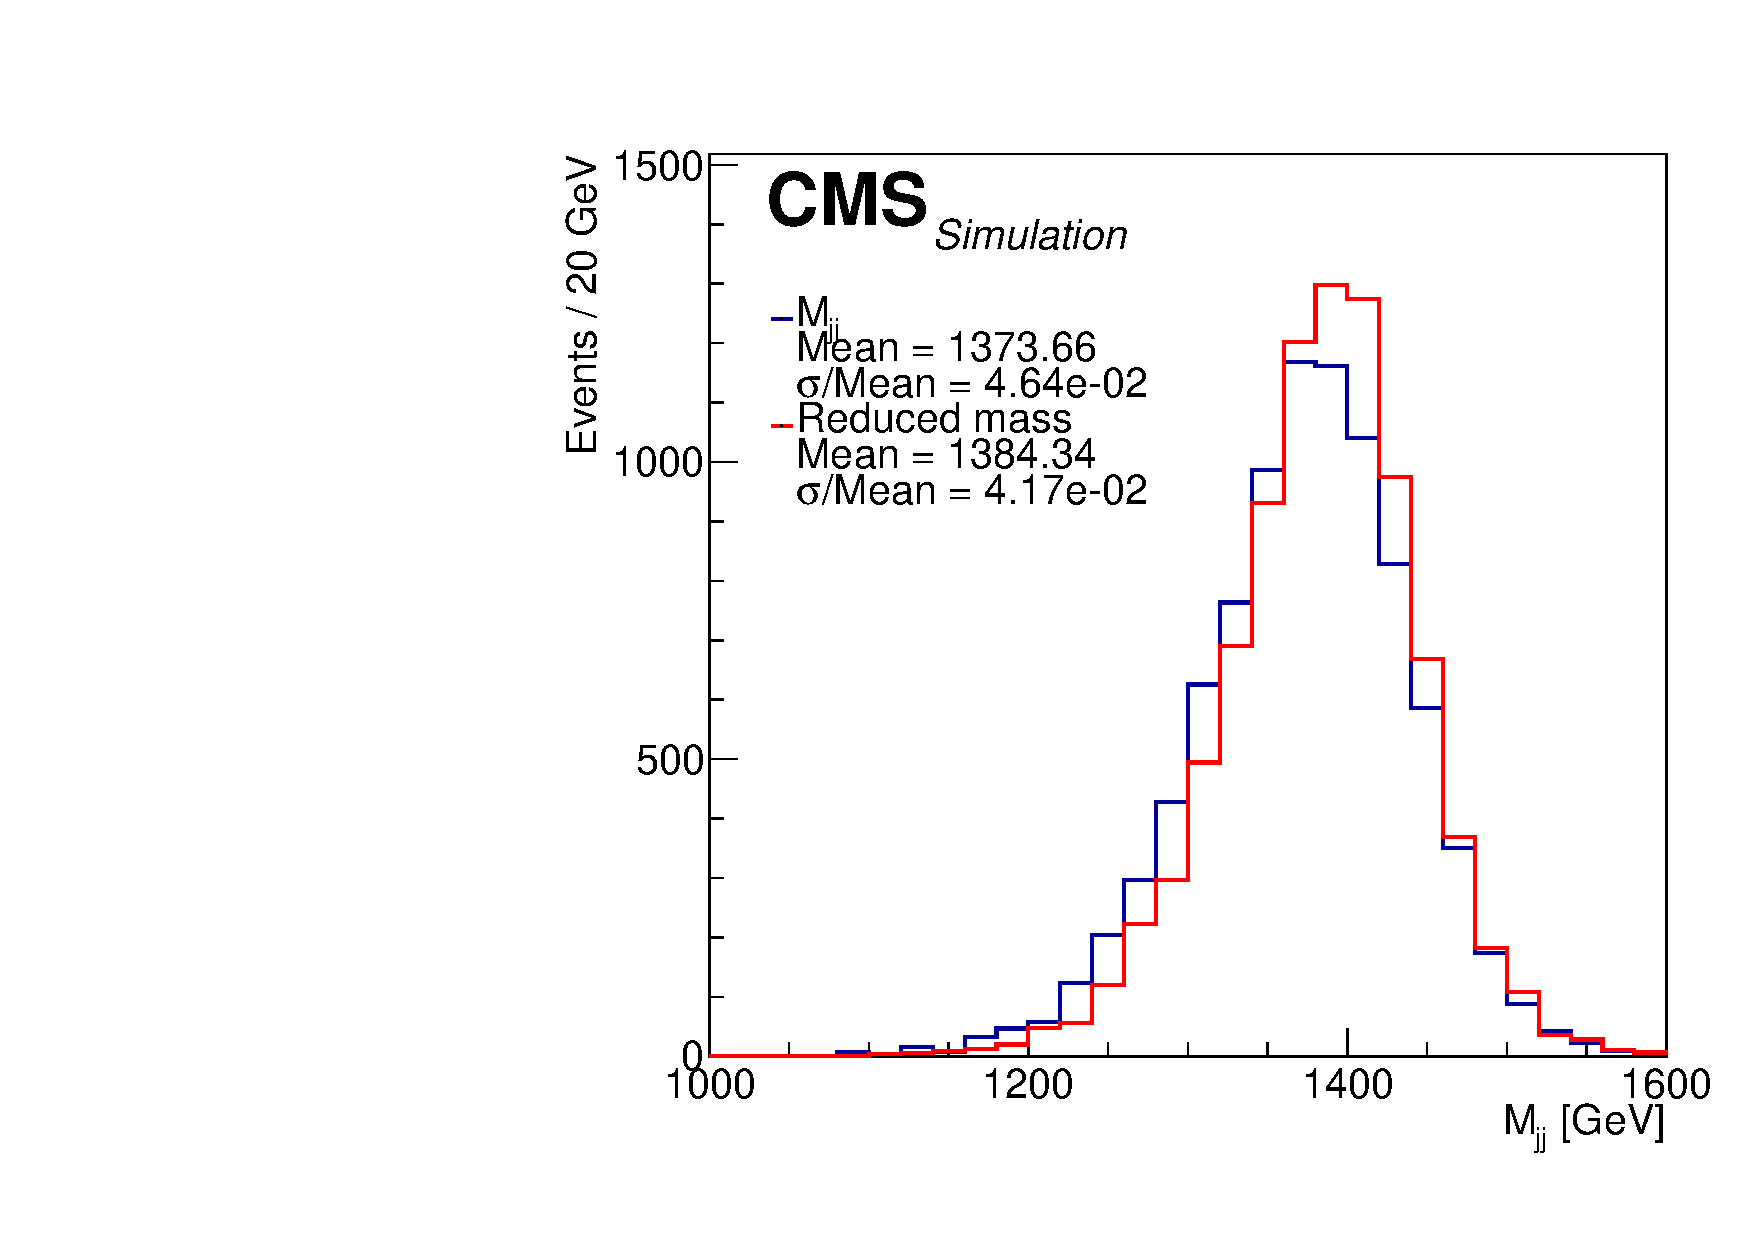
\includegraphics[width=0.5\textwidth]{Figures/red/1400.pdf} &
    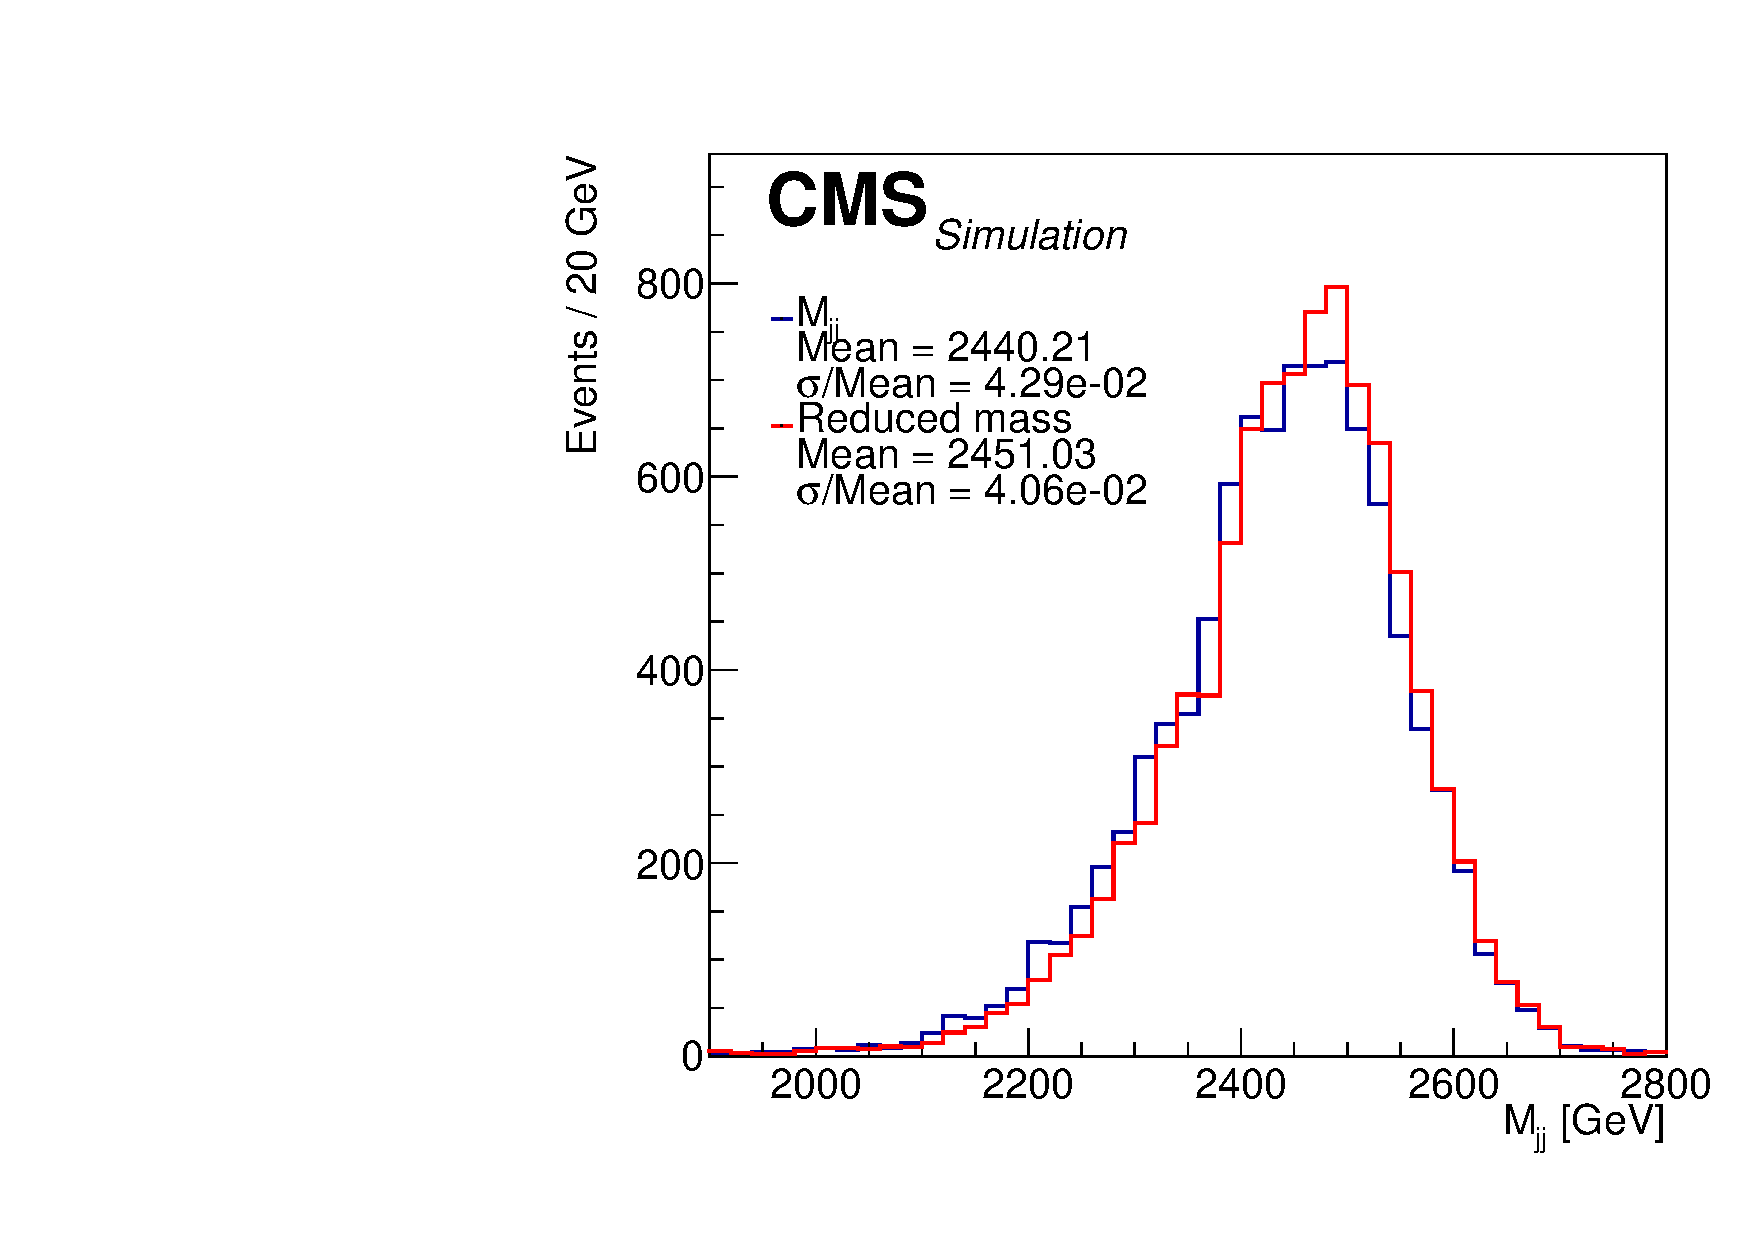
\includegraphics[width=0.5\textwidth]{Figures/red/2500.pdf} \\
    
  \end{tabular}
  \caption{The comparison of $M_{jj}$ and reduced mass distribution of bulk graviton $M_X$ = 1.4 (left) and 2.5 TeV (right). The mean and the $\sigma $/mean of a Gaussian fit to the distribution are shown.}
  \label{fig:hvt_brs}
\end{figure}

\subsection{Higgs Tagging Seletion} 

%http://xxx.lanl.gov/pdf/1402.2657v2
%CMS Collaboration, “Search for heavy resonances in the W/Z-tagged dijet mass spectrum at 13 TeV”, CMS Analysis Note CMS-AN-16-235, CERN, 2016.
%PUPPI soft-drop mass with W boson generator level correction & 105$<$ and $<$135 \\
The soft-drop procedure is inplemented to re-cluster the jet by removing soft contribution as follow\citep{Larkoski:2014wba}
\begin{itemize}
\item Deculster a targeted jet into two sub-jets.
\item Continue to decompose the sub-jets until the condition is achieved
\begin{equation} \label{eq5}
\begin{split}
\frac{min(p_{T1},p_{T2})}{p_{T1}+p_{T2}} > Z_{cut} \times (\frac{\Delta R_{12}}{R_0})^{\beta}, 
\end{split}
\end{equation}
where $R_0$ is the cone size of the original cluster algorithm, $p_T$ are the transverse momenta of two sub-jets, $\Delta R_{12}$ is the distance of two sub-jets in $\eta \phi$ space, and $Z_{cut}$ and $\beta $ are parameters. 
\item The unsplit singelet particle at the end will either be removed or remain preserved.
\end{itemize} 
If $\beta  >$ 0, the soft contribution is removed while remain a fraction of soft-collinear radiation. 
If $\beta  <$ 0, soft drop removes both soft and collinear radiation.
In CMS, the $Z_{cut}$ and $\beta $ are set 0.1 and zero respectively.
The difference between the peak of the distribution of mass of PUPPI soft-drop jets and the mass of physical Higgs boson is found\citep{CMS-AN-16-235}.
A Correction is applied to move the peak to the true phyiscal value. 
The ratio is derived by peak of the mass distribution of reconstructed jets in WW dijet Monte Carlo simulations to mass of true physical value.
The corrected PUPPI soft-drop mass of the first two leading jets are required between 105 and 135 GeV, which has been optimized.
 
%https://arxiv.org/abs/1011.2268
%https://arxiv.org/pdf/1108.2701
%https://arxiv.org/abs/1004.2489
%https://twiki.cern.ch/twiki/bin/view/CMS/JetWtagging#Working_points_and_scale_factors
%$\tau$21 & $<$ 0.55 \\
The ratio $\tau _N $ to $\tau _{N-1}$ is used as a discriminant to seperate the boosted events decaying into N particles from multi-jet events. $\tau _N $ is so-called "N-subjettiness" algorithm\citep{Thaler:2010tr,Thaler:2011gf,Stewart:2010tn}
\begin{equation} \label{eq6}
\begin{split}
\tau _N = \frac{1}{d_0} \sum\limits_{k}  p_{T,k} min \{ \Delta R_{1,k},\Delta R_{2,k},\cdots,\Delta R_{N,k} \} \\
d_0 = \sum\limits_{k}  p_{T,k} R_0,
\end{split}
\end{equation}
where k runs over the constituent particles in a given jet, $\Delta R_{jk}$ is the distance between particle j and k in $\eta \phi$ space, $R_0$ is the cone size of the original cluster algorithm. In the analysis, the boosted jets are decaying into two sub-jets, so $\tau _2 $ to $\tau _1$ ratio is used, and it is referred as $\tau _{21}$ in the following chapters.
The $\tau _{21}$ is required to be less than 0.55.  
The working point and simualtion-to-data scale factor is derived by JME POG\citep{WTagTWikiWPs}.

The double-b tagger is a multiple variable analysis discriminant used to identify b-flavor jets\citep{CMS-PAS-BTV-15-002}. Jets in multi-jet evetns and Higgs jets decaying into $b\bar{b}$ are used for training. Here lists out the input information:
\begin{itemize}
\item The first four impact paramters to its uncertainty values ordered from the largest to the smallest.
\item The  N-subjettiness axes referred as $\tau $-axes use the information of N-subjettiness
\item The first two impact parameters to its uncertainty values of $\tau $-axes ordered from the largest to the smallest.
\item The meausured significance of impact parameters of the first two tracks whose mass of secondary vertex is above buttom quark threshold.
\item The number of secondary verteces of the jet.
\item The significance of two dimenisional distance between the primary vertex and the secondary vertex and flight distance of the secondary vertex with smallest three dimenisional distance uncertainty for each $\tau $-axes.
\item $\Delta R$ of the two secondary verteces with smallest three dimenisional distance uncertainty for each $\tau $-axes.
\item The $\tau $-axis of the two secondary verteces with smallest three dimenisional distance uncertainty for each $\tau $-axes.
\item The sum of the mass of the secondary verteces associated to the $\tau $-axis for each $\tau $-axes.
\item The sum of energy of secondary verteces associated to the $\tau $-axis for each $\tau $-axes.
\item The relative pseudorapidity of three tracks of leading secondary vertex with respect to their $\tau $-axis for each $\tau $-axes.
\item The sum of energy of all tracks in the AK8 jet.
\item The z variable, defined as: 
\begin{equation} \label{eq7}
\begin{split}
z = \Delta R (SV_0, SV_1) \times \frac{p_{T,SV_1}}{m(SV_0,SV_1)}, 
\end{split}
\end{equation}
where $SV_0$ and $SV_1$ are the secondary verteces with the smallest 3D flight distance uncertainty.
\end{itemize} 
%https://cds.cern.ch/record/2195743
%https://twiki.cern.ch/twiki/bin/viewauth/CMS/BtagRecommendation80XReReco
The double-b working points and simualtion-to-data scale factor is derived by BTV POG\citep{BtagRecommendation80XReReco}.
The analysis is seperated into two catgory with two Higgs jets in the events either both passing loose working point ($>$ 0.3) or both passing tight working point ($>$ 0.8), which are referred as LL and TT categories respectively. The events sit in TT region will be excluded from LL region to make two categories orthogonal.
%double-b tagger & $>$0.3 or $>$0.8 \\



\section{Triggers} \label{Triggers}
Since the final state includes di-Higgs jets, the triggers are selected considering the requirements on the scale sum of the energy of external partons $H_T$, |$\Delta \eta $(the first two leading jets)|, M$_{jj}$, $p_T$, the groomed mass of the jets, and double-b tagger. PFHT900 is used to supplement the inefficiency of PFHT800 in period H of data taking.
\begin{table}[h!]
  \begin{center}
    \begin{tabular}{l}
    Triggers \\
    \hline
    HLT$\_$PFHT800 \\
    HLT$\_$PFHT900 \\
    HLT$\_$PFHT650$\_$WideJetMJJ900DEtaJJ1p5 \\
    HLT$\_$AK8PFJet360$\_$TrimMass30 \\
    HLT$\_$AK8DiPFJet280$\_$200$\_$TrimMass30$\_$BTagCSV$\_$p20 \\
    HLT$\_$AK8PFHT650$\_$TrimR0p1PT0p03Mass50 \\
    \hline
    \end{tabular}
  \end{center}

  \caption{List of Triggers applied in the analysis.}
\end{table} 

\begin{table}[h!]
  \begin{center}
    \begin{tabular}{ll}
    Selection & Requirement \\
    \hline
    Number of good vertex & $>$ 1 \\
    MET Filters & AND of all filters\\
	Trigger & OR of all triggers\\
	Lepton veto & one tight-tagged or two loose-tagged \\
    $p_{T}$ of AK8 jets & $>$ 300GeV \\
	|$\eta$| of AK8 jets & $<$ 2.4 \\
	Tight LepVeto jet ID & pass \\
	|$\Delta \eta $ (two AK8 jets) | & $<$ 1.3 \\
	Reduce mass & $>$ 750 GeV \\
	corrected PUPPI soft-drop mass & 105 $<$ and $<$ 135 \\
	$\tau _{21}$ & $<$ 0.55 \\
	double-b tagger & $>$ 0.3 (LL) or $>$ 0.8 (TT)\\
	\hline
    \end{tabular}
  \end{center}

  \caption{List of all selection in the analysis.}
\end{table} 

\begin{table}[h!]
  \begin{center}
    \begin{tabular}{lllllllllll}
    $M_X$ & Trig. & Jet $p_T$, $\eta$ & Veto$_{lep}$ & $\Delta \eta$ & Lepton & $\tau _{21}$ & $M_{AK8}$ & $M^{red}_{jj}$ & LL & TT\\
    \hline
750 & 0.432 & 0.248 & 0.247 & 0.213 & 0.213 & 0.093 & 0.029 & 0.024 & 0.016 & 0.009 \\
800 & 0.547 & 0.367 & 0.367 & 0.327 & 0.326 & 0.152 & 0.051 & 0.050 & 0.036 & 0.021 \\
900 & 0.693 & 0.552 & 0.552 & 0.487 & 0.485 & 0.245 & 0.083 & 0.083 & 0.061 & 0.033 \\
1000 & 0.772 & 0.666 & 0.666 & 0.552 & 0.550 & 0.296 & 0.101 & 0.101 & 0.075 & 0.041 \\
1200 & 0.859 & 0.792 & 0.792 & 0.585 & 0.584 & 0.335 & 0.116 & 0.116 & 0.084 & 0.044 \\
1400 & 0.902 & 0.854 & 0.854 & 0.591 & 0.590 & 0.355 & 0.123 & 0.123 & 0.087 & 0.044 \\
1600 & 0.928 & 0.890 & 0.889 & 0.592 & 0.591 & 0.358 & 0.124 & 0.124 & 0.086 & 0.041 \\
1800 & 0.946 & 0.913 & 0.913 & 0.595 & 0.594 & 0.365 & 0.124 & 0.124 & 0.082 & 0.036 \\
2000 & 0.957 & 0.931 & 0.931 & 0.598 & 0.598 & 0.365 & 0.127 & 0.127 & 0.081 & 0.036 \\
2500 & 0.975 & 0.956 & 0.955 & 0.596 & 0.595 & 0.367 & 0.125 & 0.125 & 0.076 & 0.030 \\
3000 & 0.981 & 0.966 & 0.965 & 0.589 & 0.589 & 0.357 & 0.123 & 0.123 & 0.068 & 0.022 \\
3500 & 0.987 & 0.973 & 0.972 & 0.582 & 0.582 & 0.349 & 0.116 & 0.116 & 0.059 & 0.018 \\
4500 & 0.991 & 0.977 & 0.976 & 0.579 & 0.578 & 0.334 & 0.103 & 0.103 & 0.044 & 0.010 \\
\hline
    \end{tabular}
  \end{center}
	
  \caption{The cut flow of all $M_X$ (GeV) of spin-0 radion.}
\end{table} 

\begin{table}[h!]
  \begin{center}
    \begin{tabular}{lllllllllll}
    $M_X$ & Trig. & Jet $p_T$, $\eta$ & Jet ID & $\Delta \eta$ & Veto$_{lep}$ & $\tau _{21}$ & $M_{AK8}$ & $M^{red}_{jj}$ & LL & TT\\
    \hline
    750 & 0.610 & 0.368 & 0.368 & 0.331 & 0.330 & 0.149 & 0.049 & 0.039 & 0.027 & 0.015 \\
	800 & 0.758 & 0.541 & 0.541 & 0.503 & 0.502 & 0.237 & 0.080 & 0.079 & 0.057 & 0.032 \\
	900 & 0.903 & 0.772 & 0.771 & 0.716 & 0.715 & 0.371 & 0.125 & 0.124 & 0.092 & 0.051 \\
	1000 & 0.958 & 0.885 & 0.885 & 0.801 & 0.799 & 0.434 & 0.151 & 0.151 & 0.111 & 0.062 \\
1200 & 0.988 & 0.962 & 0.961 & 0.843 & 0.842 & 0.499 & 0.178 & 0.178 & 0.129 & 0.068 \\
1400 & 0.996 & 0.984 & 0.983 & 0.854 & 0.853 & 0.524 & 0.182 & 0.182 & 0.129 & 0.064 \\
1600 & 0.998 & 0.993 & 0.993 & 0.858 & 0.857 & 0.532 & 0.186 & 0.186 & 0.128 & 0.061 \\
1800 & 0.999 & 0.996 & 0.996 & 0.864 & 0.863 & 0.543 & 0.193 & 0.193 & 0.130 & 0.059 \\
2000 & 1.000 & 0.998 & 0.998 & 0.861 & 0.860 & 0.541 & 0.190 & 0.190 & 0.123 & 0.054 \\
2500 & 1.000 & 0.999 & 0.999 & 0.862 & 0.862 & 0.538 & 0.188 & 0.188 & 0.113 & 0.044 \\
3000 & 1.000 & 1.000 & 0.999 & 0.865 & 0.865 & 0.530 & 0.186 & 0.186 & 0.102 & 0.034 \\
4000 & 1.000 & 1.000 & 0.999 & 0.861 & 0.861 & 0.505 & 0.166 & 0.166 & 0.078 & 0.021 \\
4500 & 1.000 & 1.000 & 0.999 & 0.859 & 0.858 & 0.502 & 0.156 & 0.156 & 0.065 & 0.016 \\
\hline
    \end{tabular}
  \end{center}
	
  \caption{The cut flow of all $M_X$ (GeV) of spin-2 bulk graviton.}
\end{table} 



\section{Simulation Distribution} 
In the section, distribution of Monte Carlo simulations of signal and background will be shown to demonstrate the discrimination of each variables of the seletion. For each distribution, all selection described in previous section is required except the variable itself and double-b tagger discriminant. The cross section of every signal is set to 20 pb. The numbers of events of signal and of background are normalized to same luminosity of data of 35.9fb$^{-1}$. Multi-jet events are added up by samples of different $H_T$ section listed in table 3.4, and seperated into four categories summarized in the table 3.10.  Besides, the cross sections at leading order of multi-jet events are multiplied by a factor about 0.7 to modify them closer to the value of next leading order.

\begin{table}[h!]
  \begin{center}
    \begin{tabular}{lll}
    category & hadron flavor of AK8 jets & hadron flavor of subjets \\
    \hline
    bb & 5 & 5 (both) \\
    b & 5 & 5 (only one) \\
    cc/c & 4 & 4 (at least one) \\
    light & all remaining & all remaining \\
	\hline
    \end{tabular}
  \end{center}

  \caption{List of categorization of multijet events.}
\end{table} 

\begin{figure}[t]
  \centering
  \begin{tabular}{cc}
    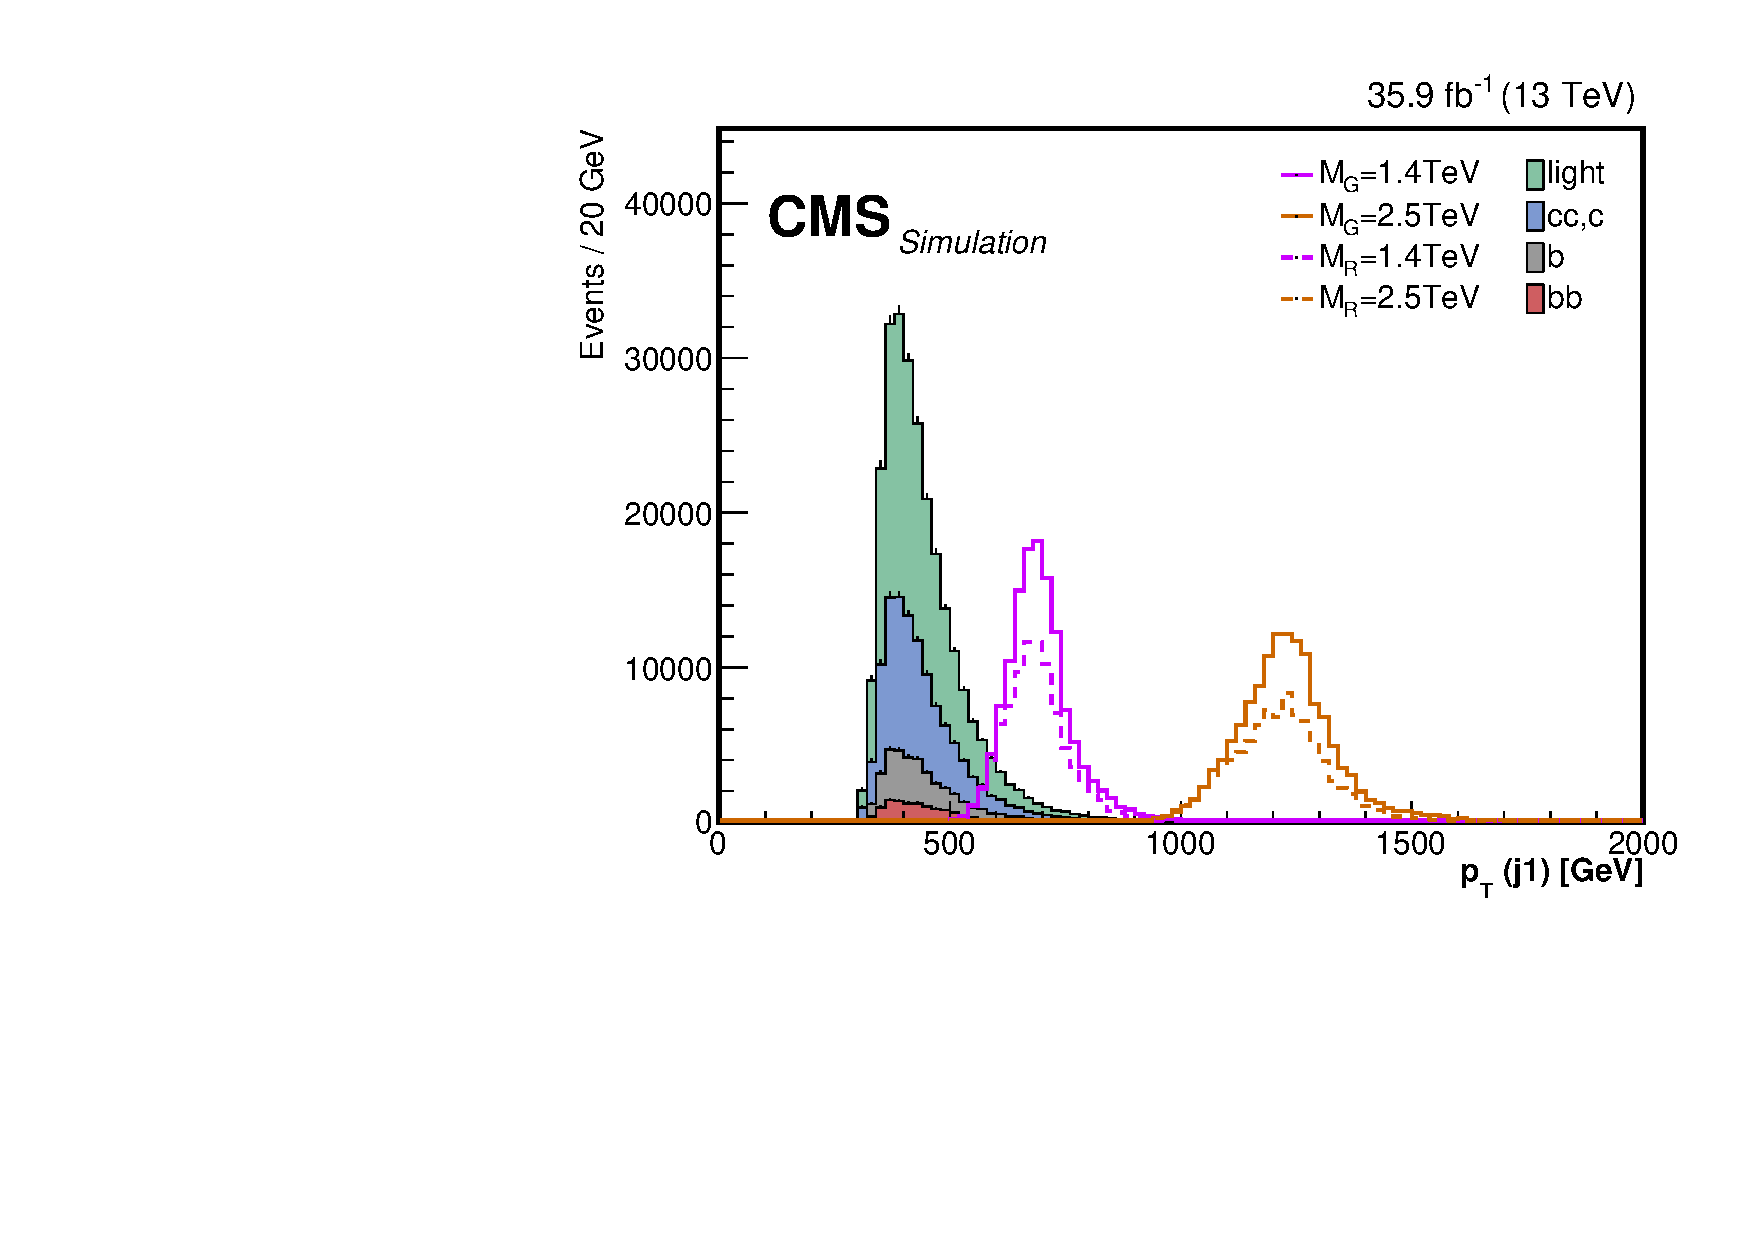
\includegraphics[width=0.5\textwidth]{Figures/MC_N1/pt_j0.pdf} &
    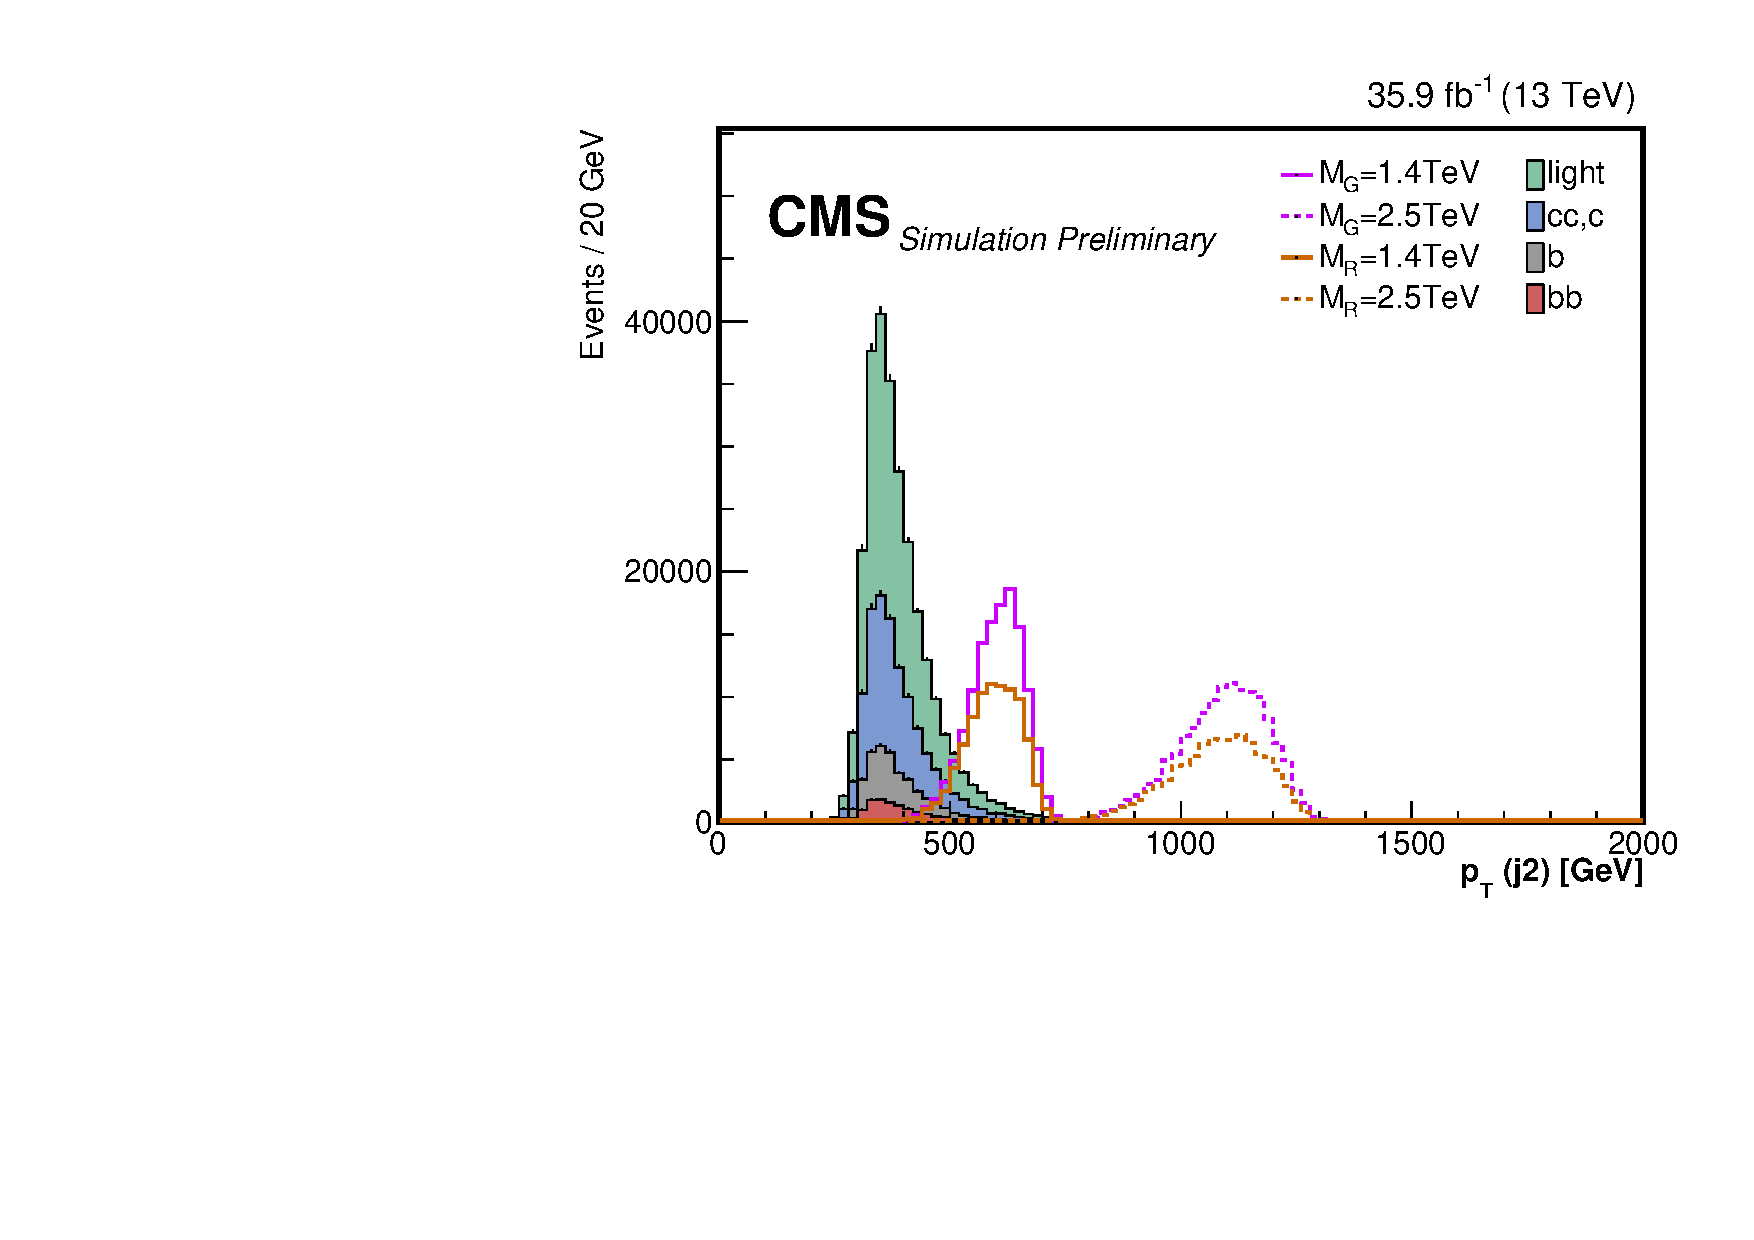
\includegraphics[width=0.5\textwidth]{Figures/MC_N1/pt_j1.pdf} \\
     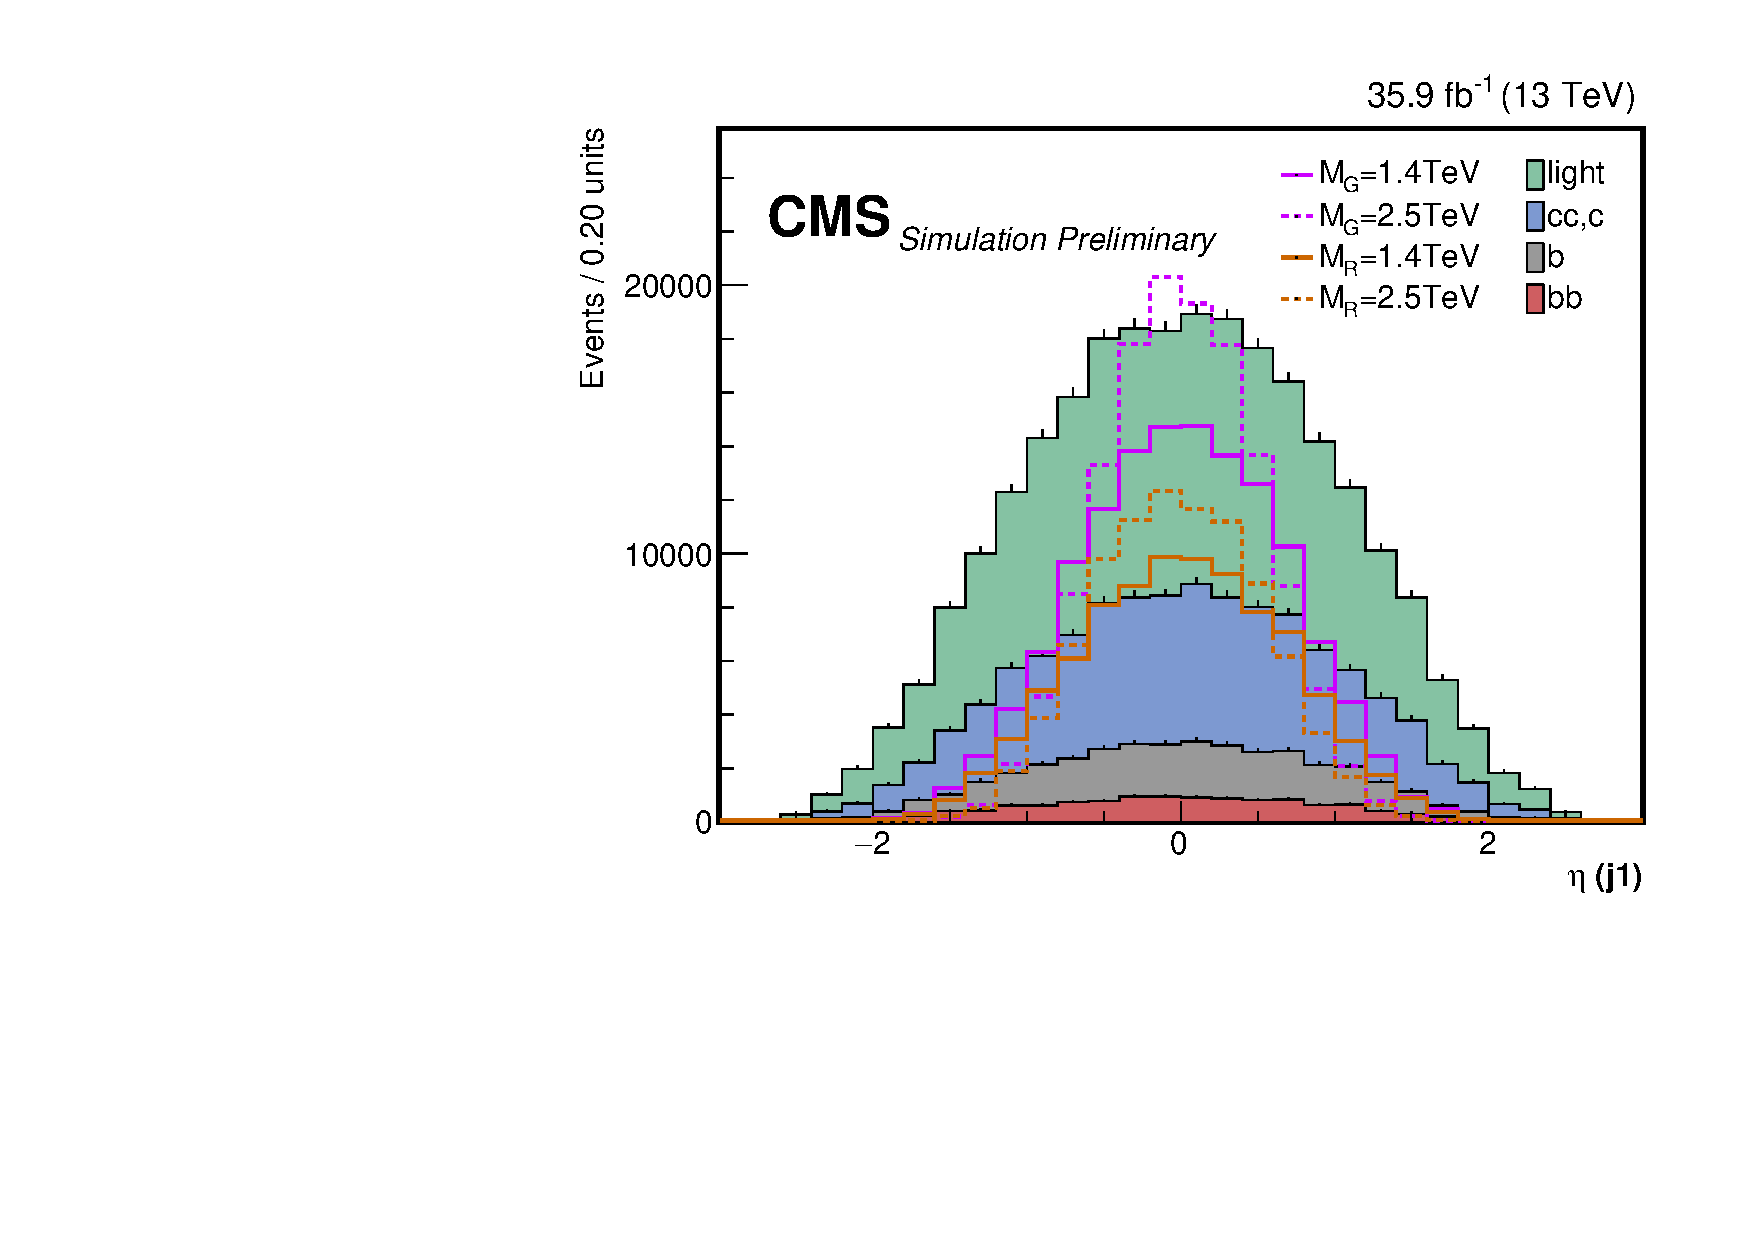
\includegraphics[width=0.5\textwidth]{Figures/MC_N1/eta_j0.pdf} &
    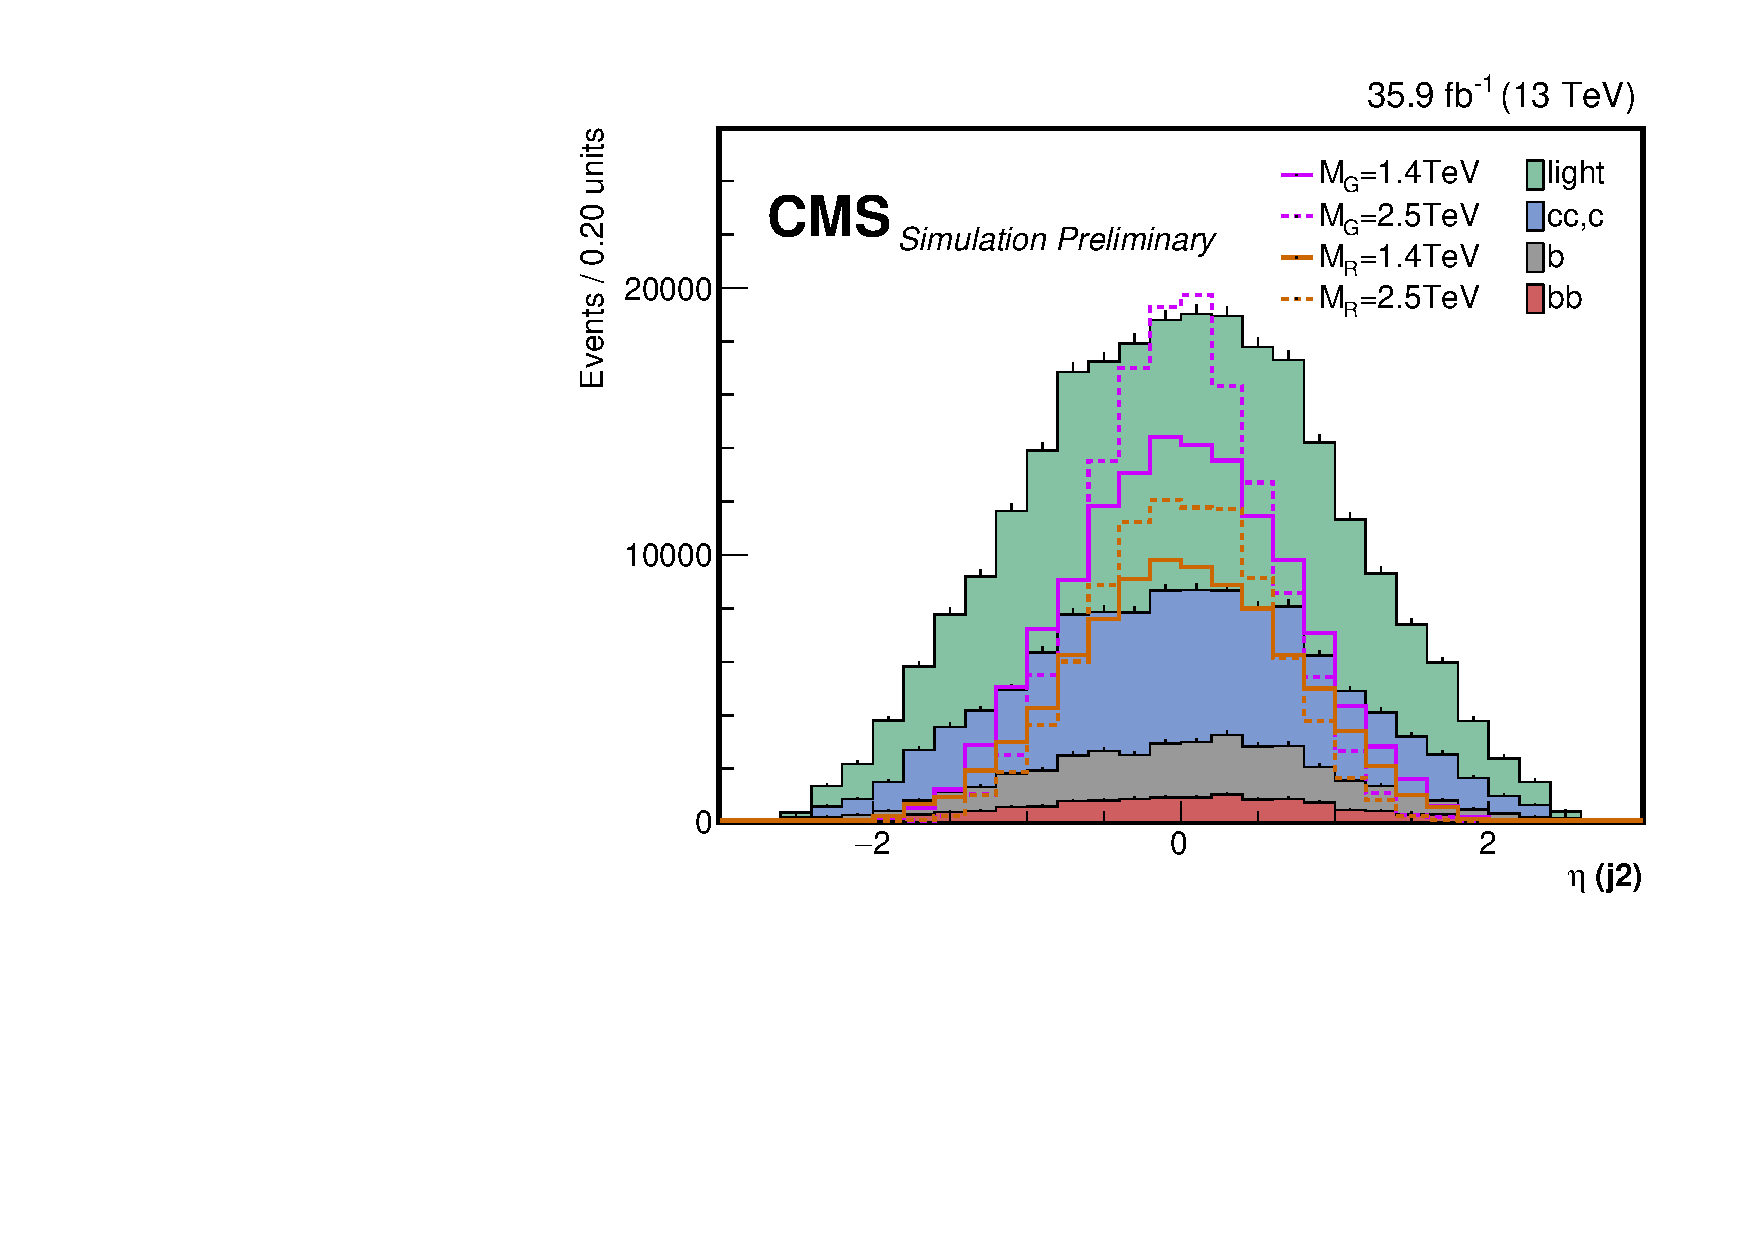
\includegraphics[width=0.5\textwidth]{Figures/MC_N1/eta_j1.pdf} \\
     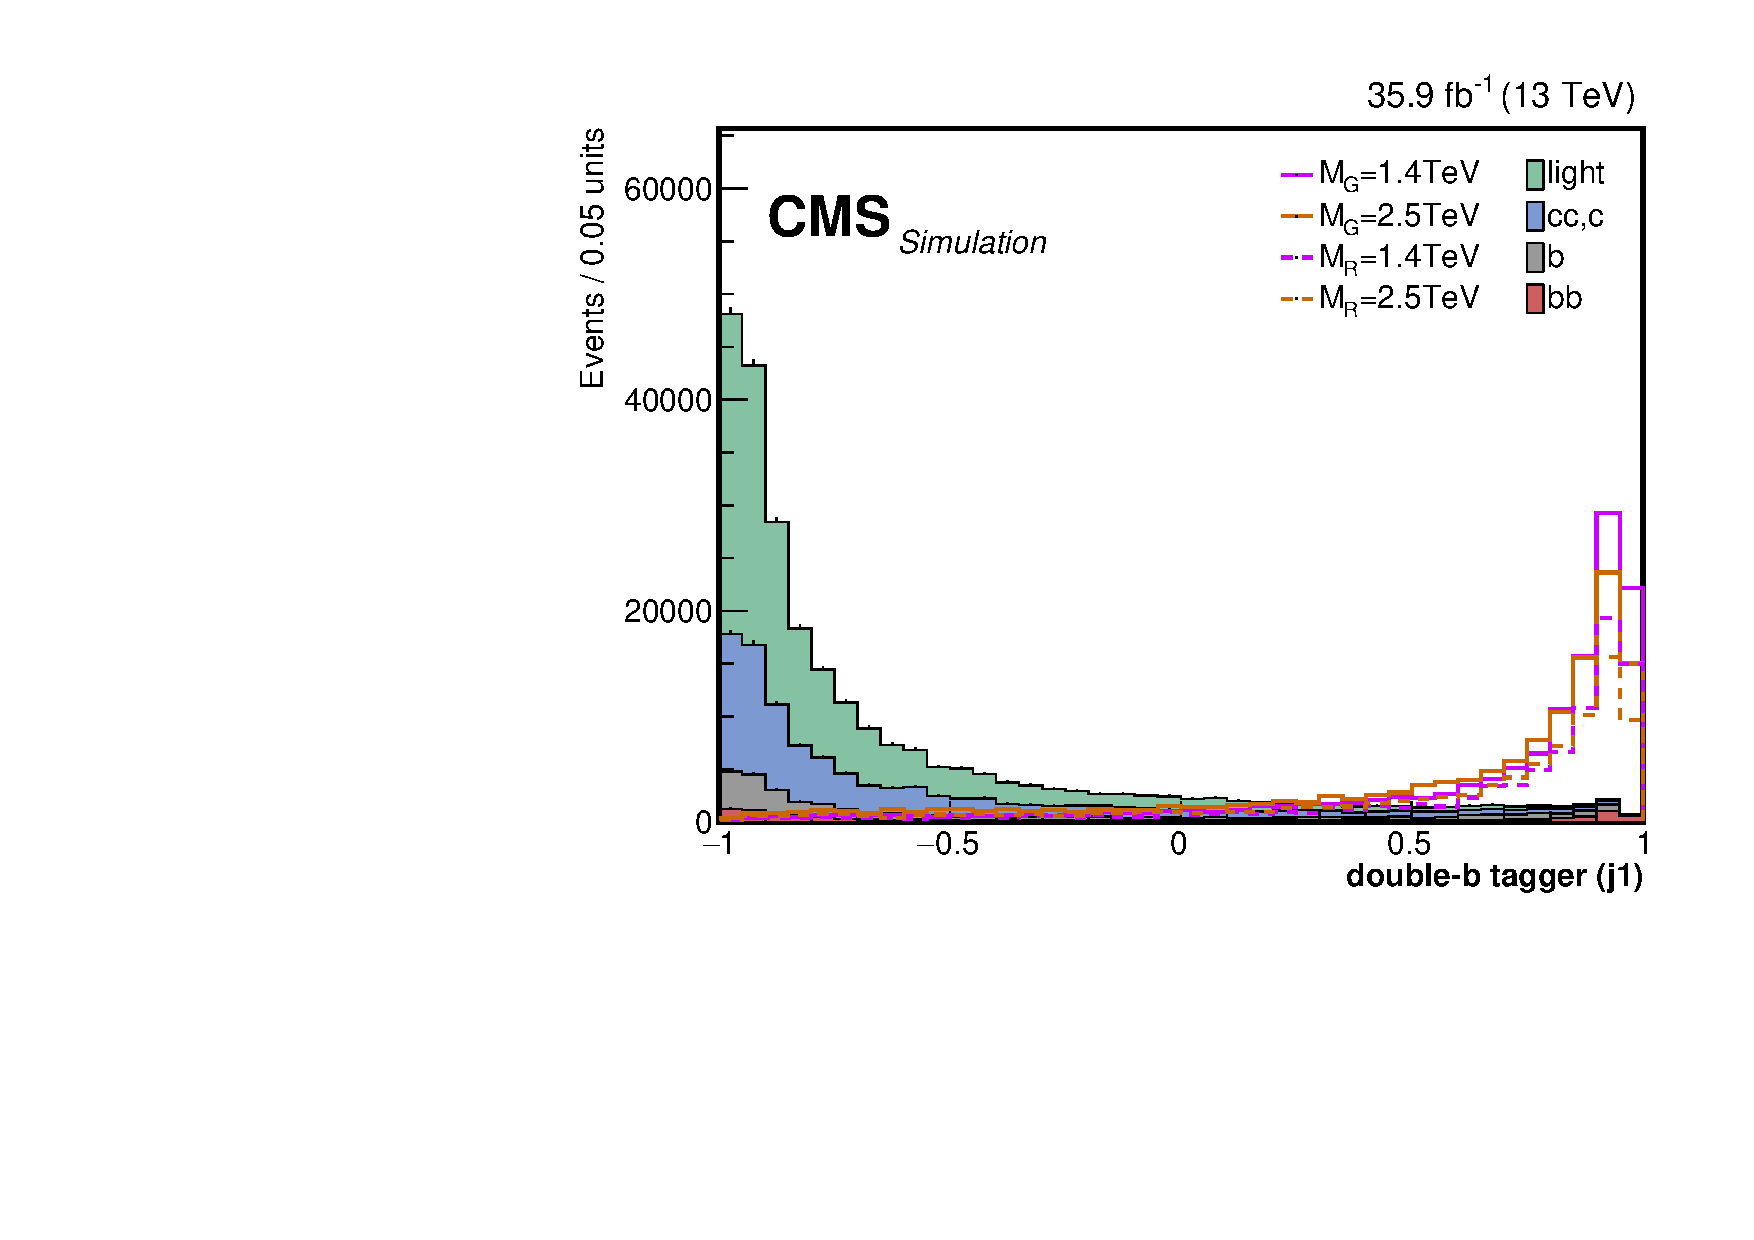
\includegraphics[width=0.5\textwidth]{Figures/MC_N1/doubleSV_j0.pdf} &
    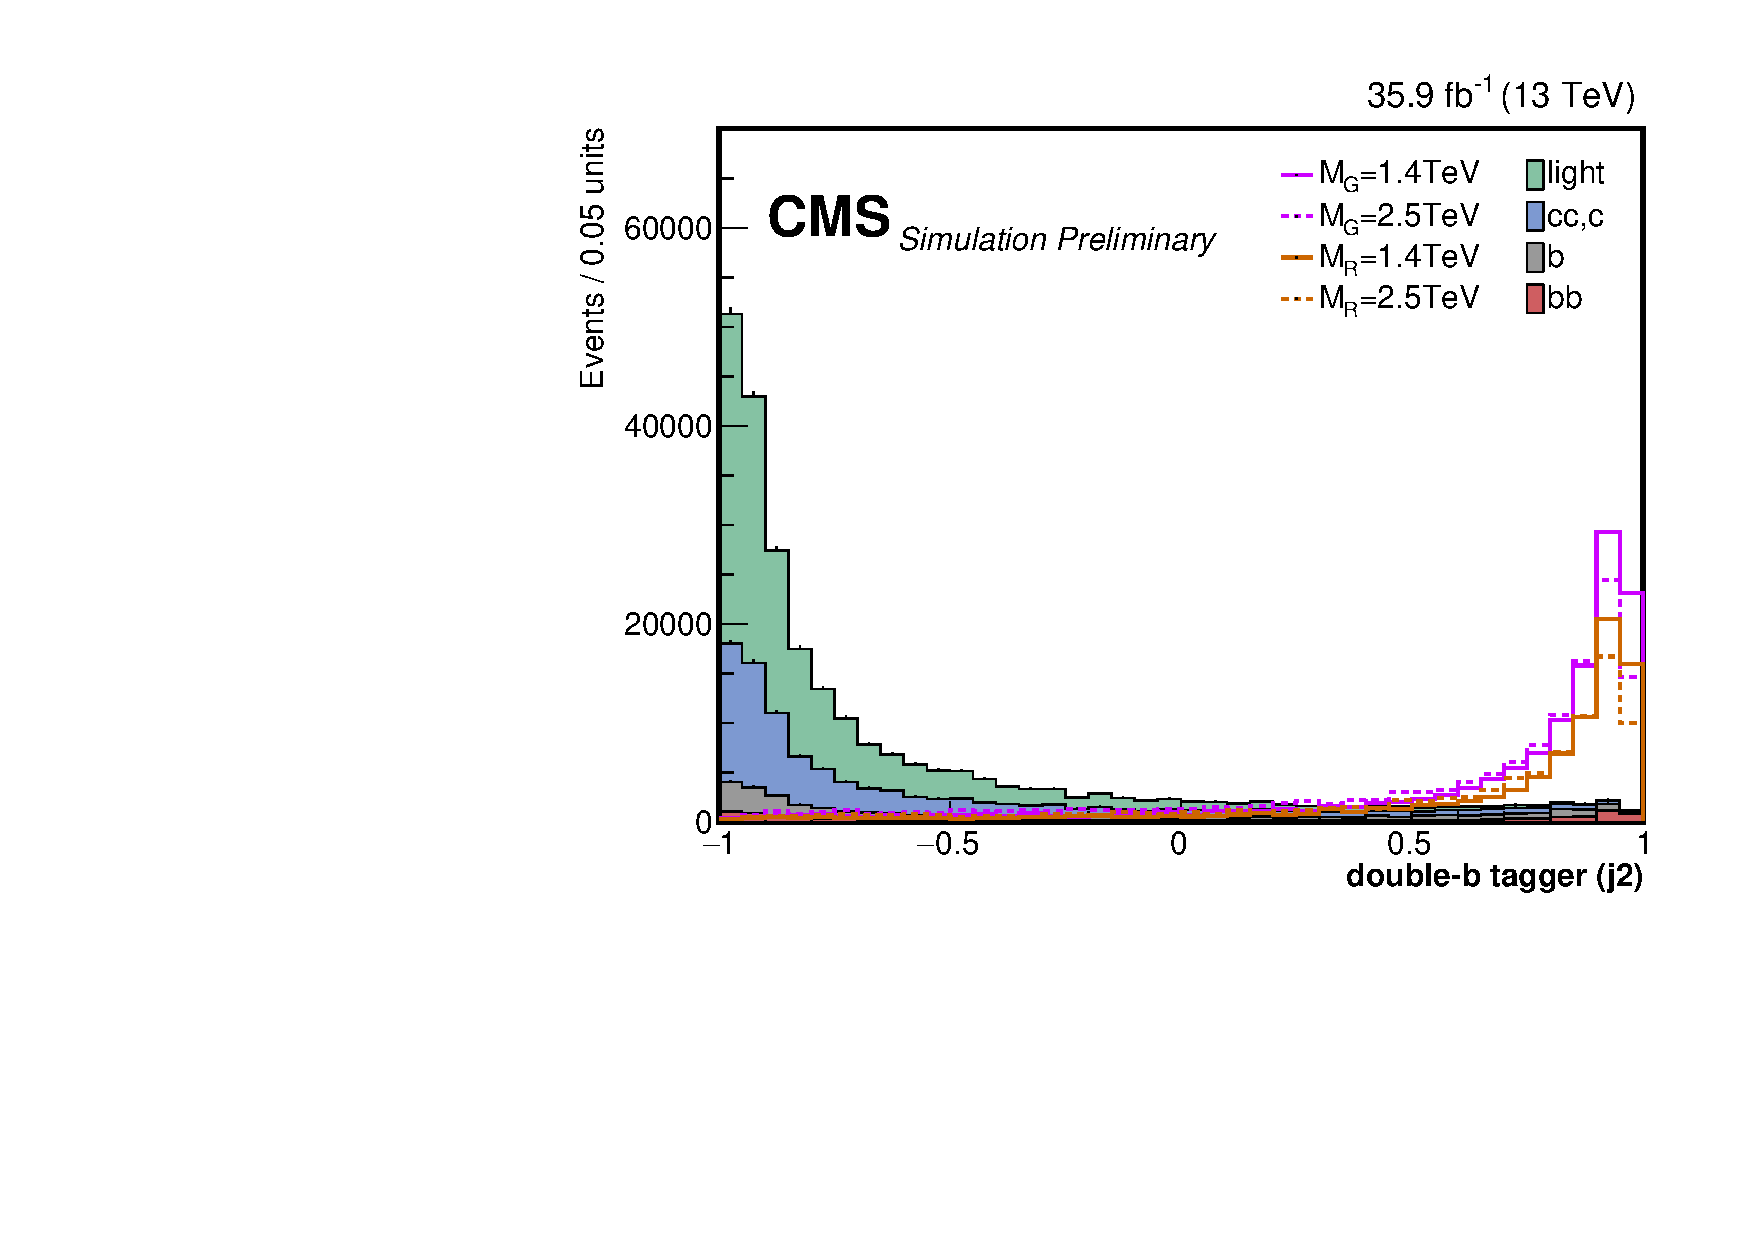
\includegraphics[width=0.5\textwidth]{Figures/MC_N1/doubleSV_j1.pdf} \\
  \end{tabular}
  \caption{The comparison of signal and background. The signals of $M_{X}$ = 1.4 TeV and 2.5 TeV from both models are shown. The cross section is set to 20 pb in the figures. Multi-jet events are seperated into four categories summarized in the table 3.10. From top to buttom are the comparison of $p_{T}$, $\eta $, and double-b tagger of leading (left) and next leading (right) AK8 jet.}
  \label{fig:hvt_brs}
\end{figure}

\begin{figure}[t]
  \centering
  \begin{tabular}{cc}
    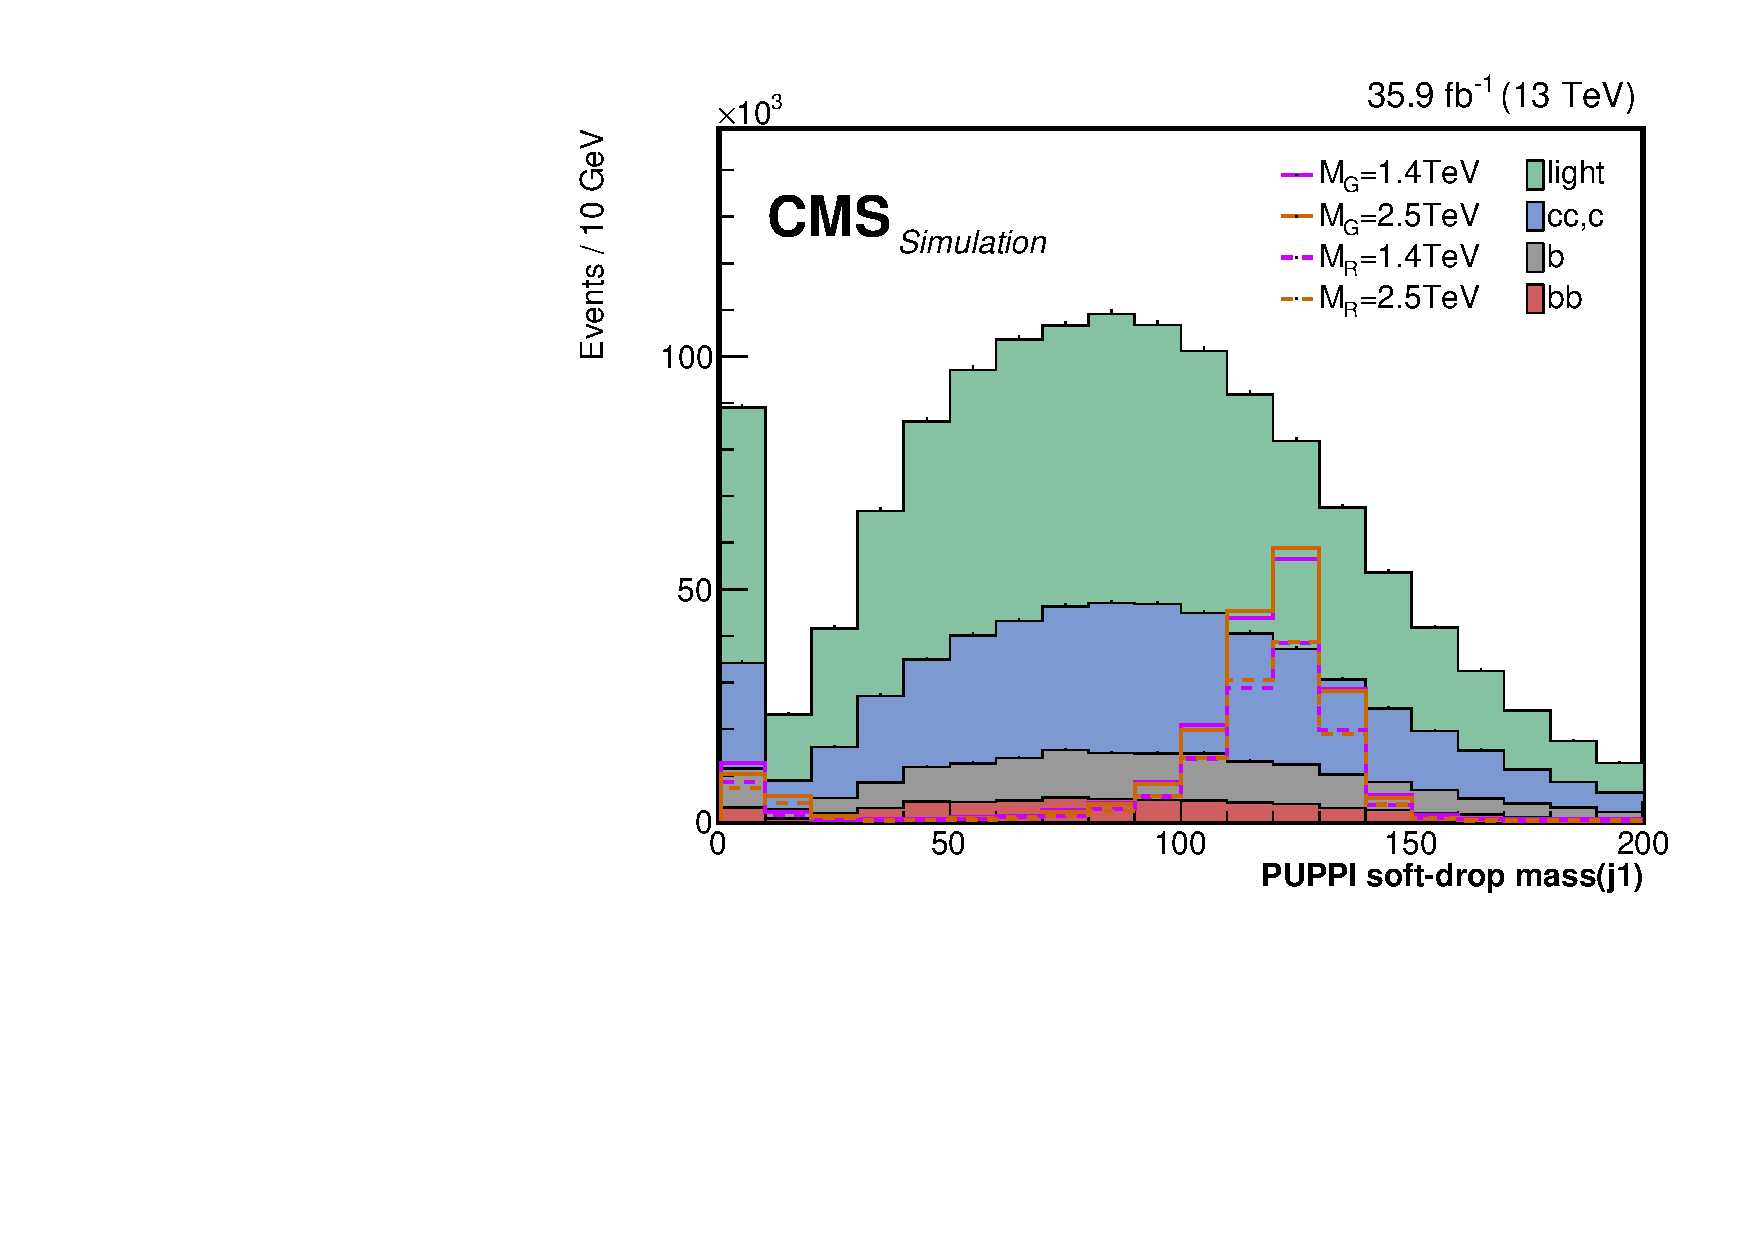
\includegraphics[width=0.5\textwidth]{Figures/MC_N1/puppiSDMassThea_j0.pdf} &
    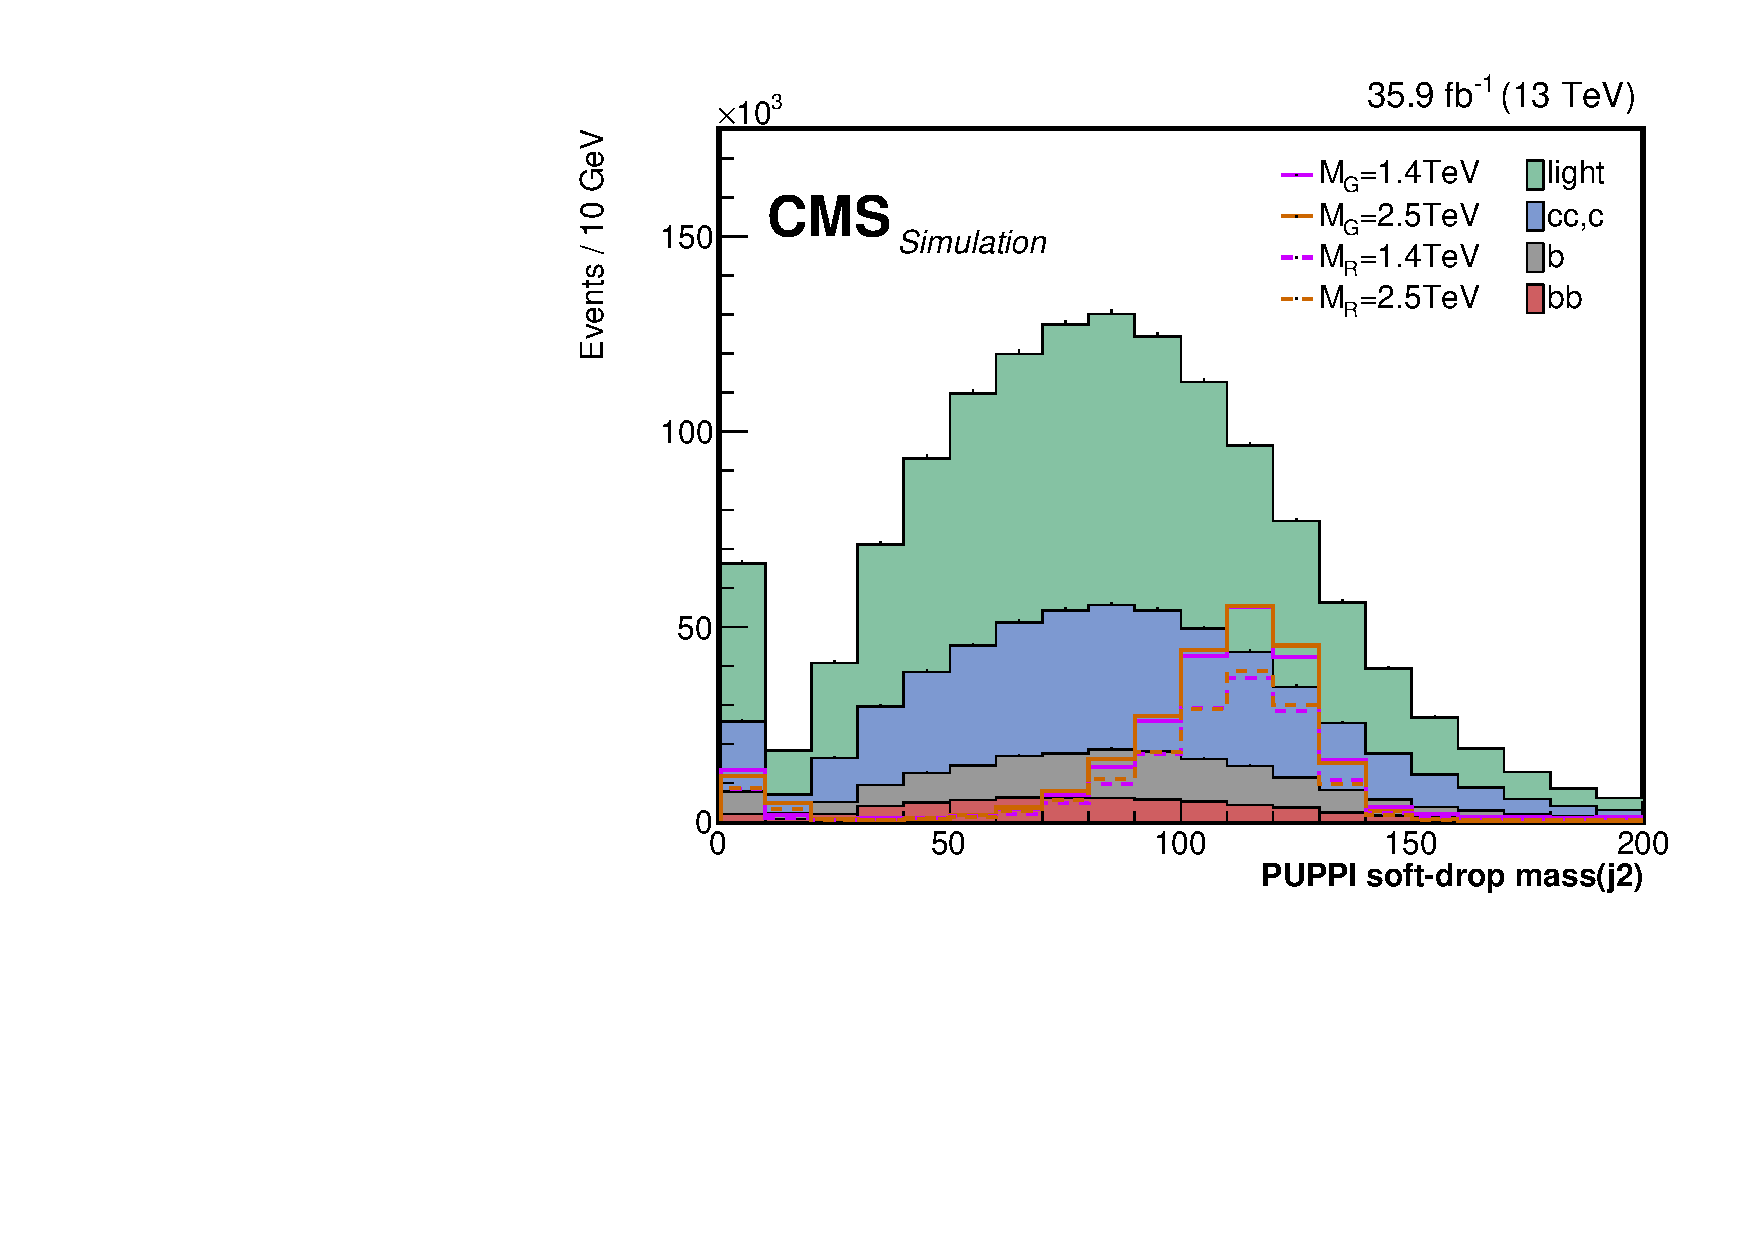
\includegraphics[width=0.5\textwidth]{Figures/MC_N1/puppiSDMassThea_j1.pdf} \\
     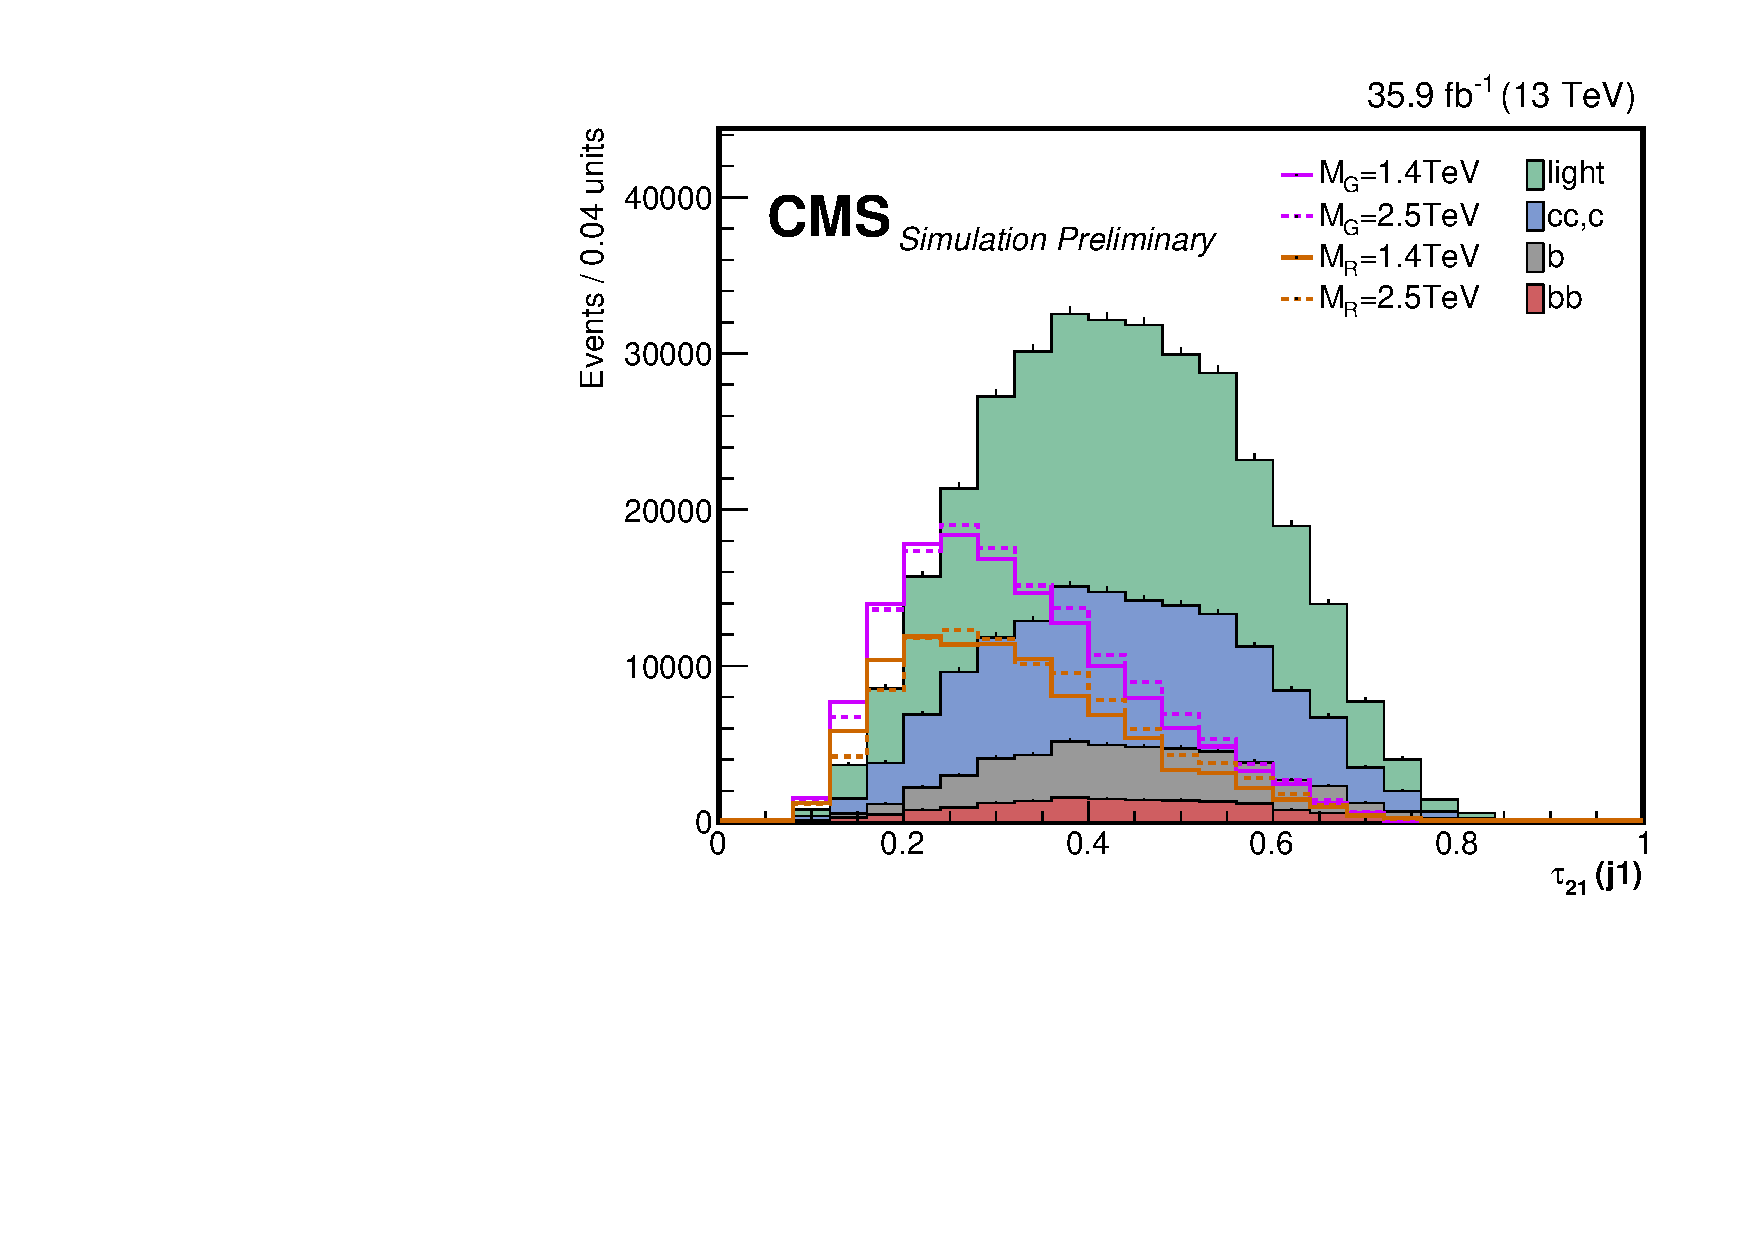
\includegraphics[width=0.5\textwidth]{Figures/MC_N1/puppiTau21_j0.pdf} &
    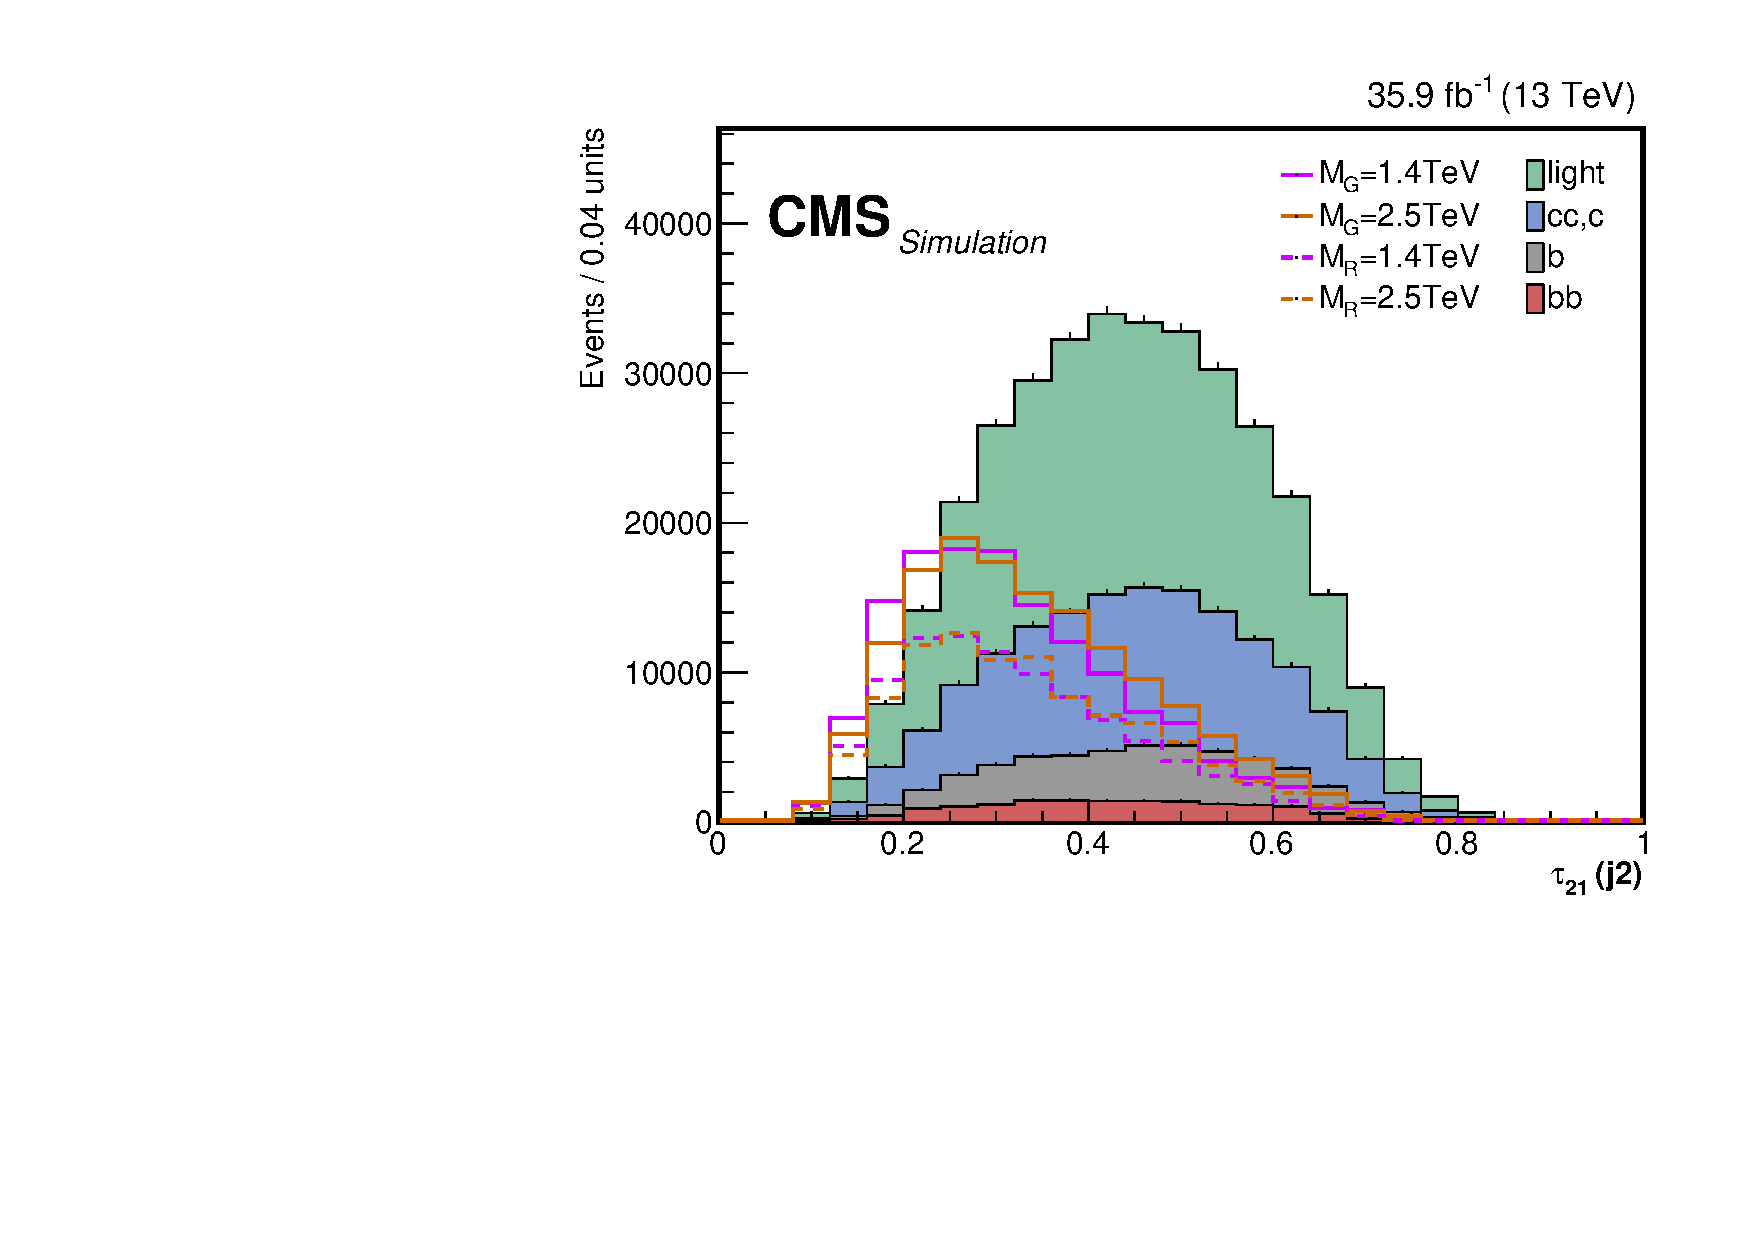
\includegraphics[width=0.5\textwidth]{Figures/MC_N1/puppiTau21_j1.pdf} \\
     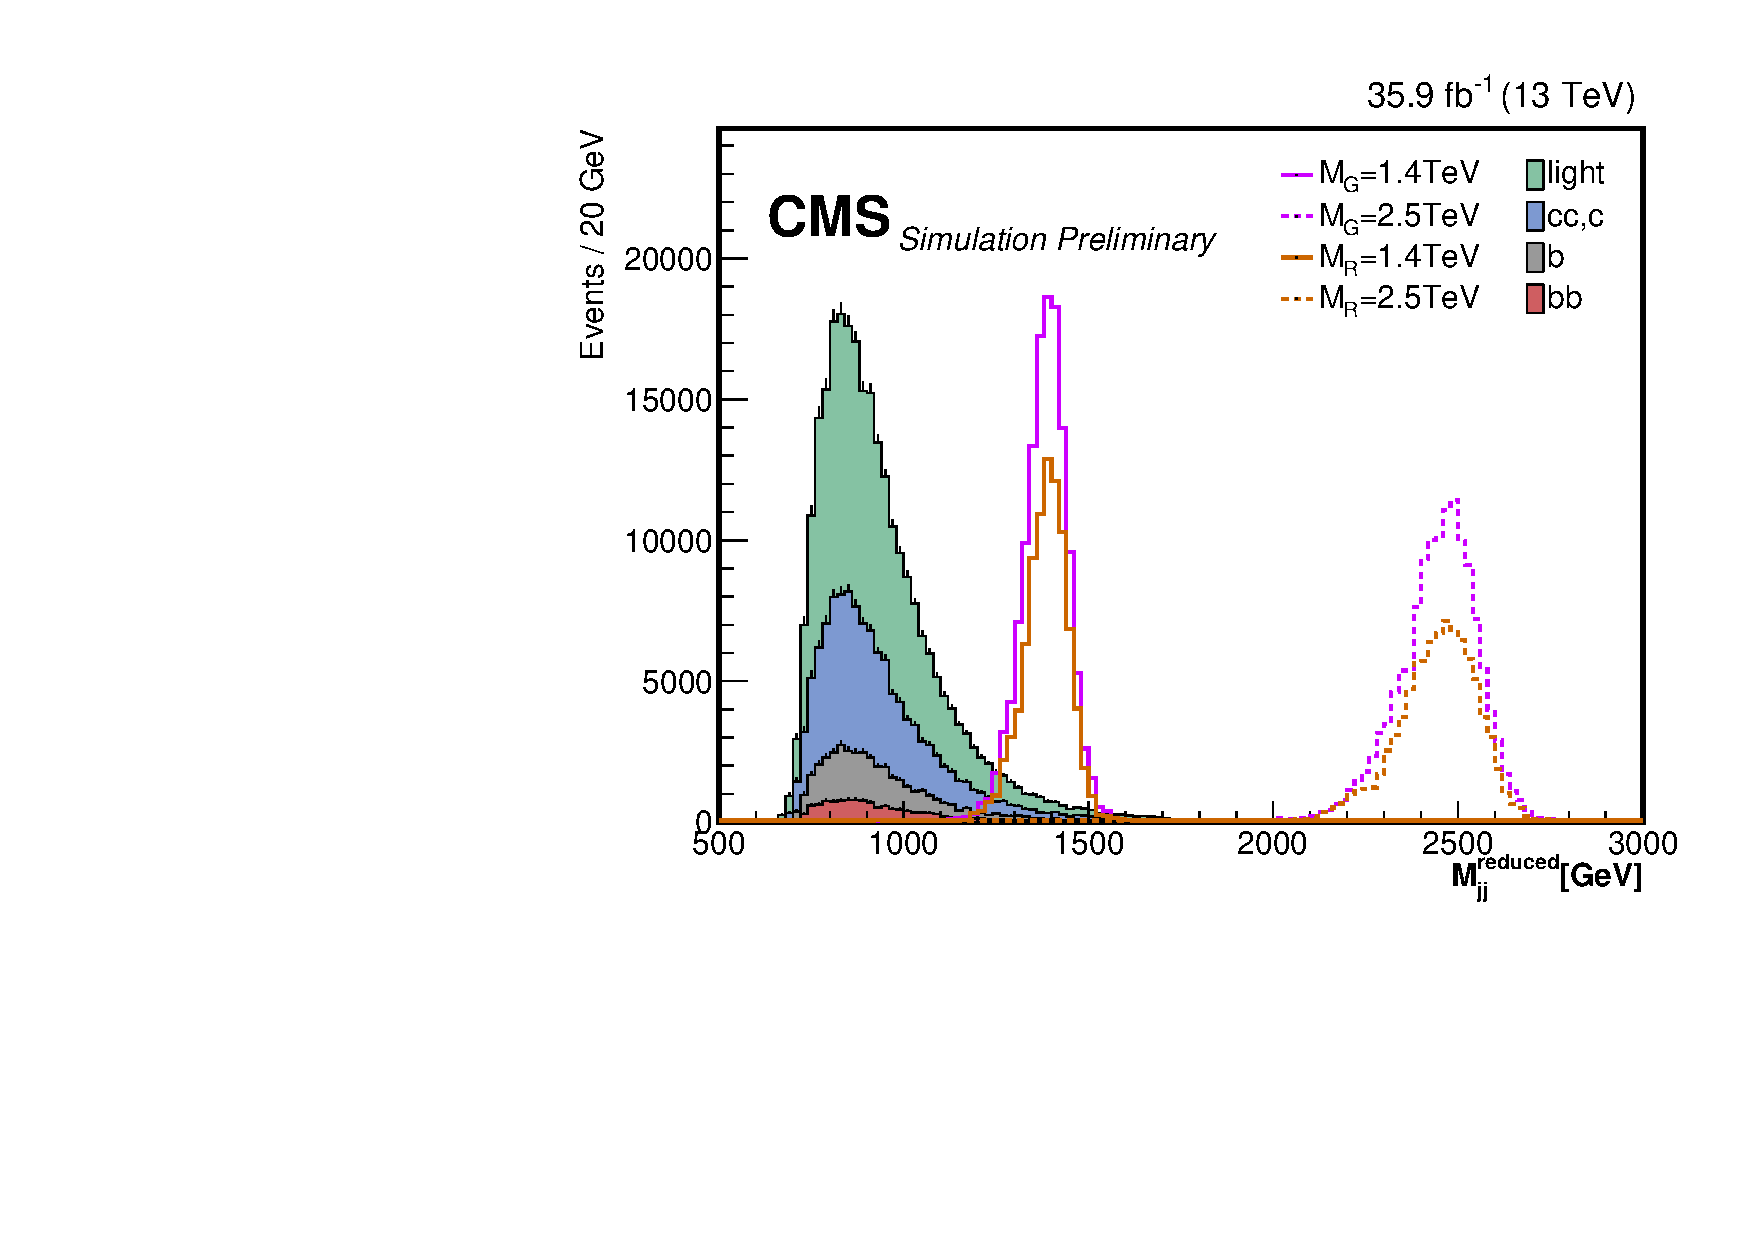
\includegraphics[width=0.5\textwidth]{Figures/MC_N1/totalMassRed.pdf} &
    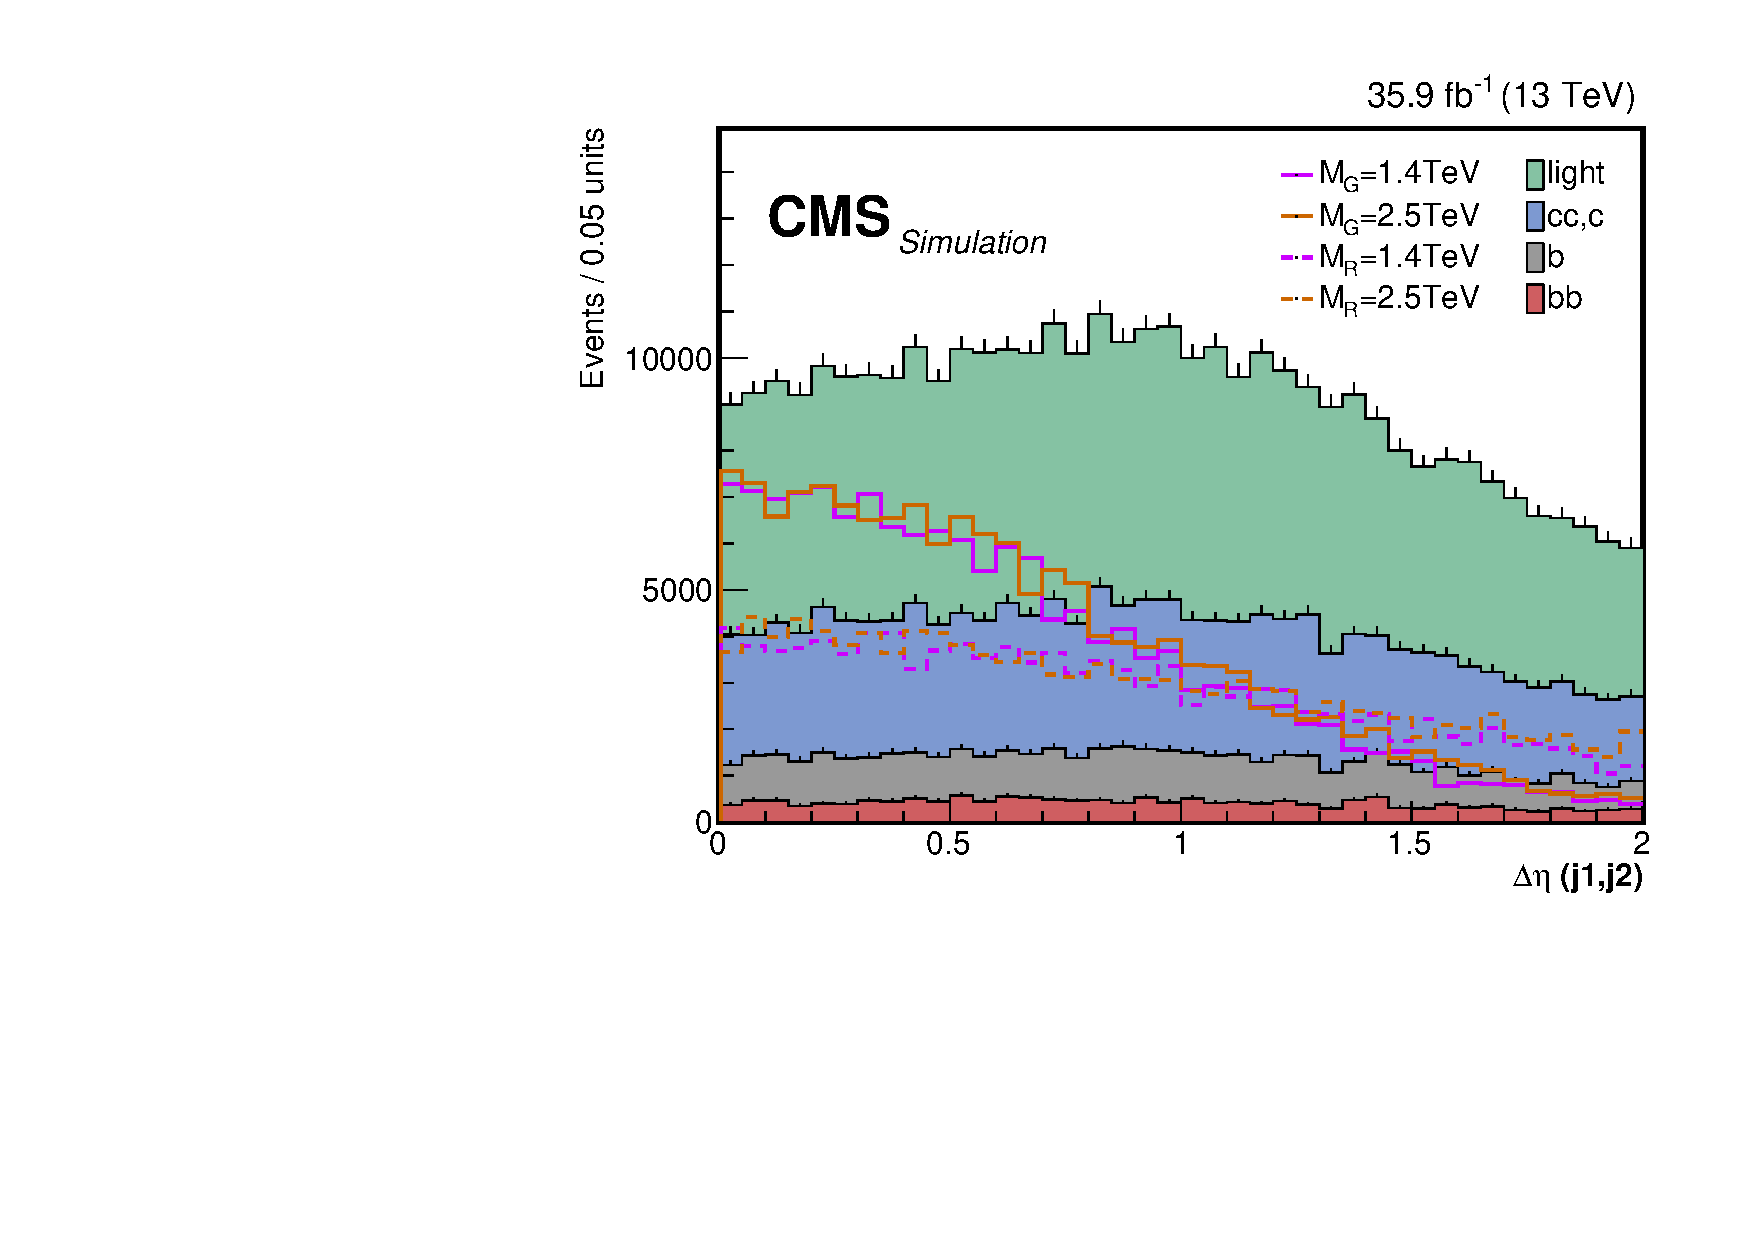
\includegraphics[width=0.5\textwidth]{Figures/MC_N1/deltaEta.pdf} \\
  \end{tabular}
  \caption{The comparison of signal and background. The signals of $M_{X}$ = 1.4 TeV and 2.5 TeV from both models are shown. The cross section is set to 20 pb in the figures. Multi-jet events are seperated into four categories summarized in the table 3.10. From top to buttom are the comparison of PUPPI soft-drop mass, $\tau _{21}$ of leading (left) and next leading (right) AK8 jet, the reduced mass (buttom left), and |$\Delta \eta $ (the two leading AK8 jets)| (buttom right).}
  \label{fig:hvt_brs}
\end{figure}

\section{Data and Monte Carlo Comparison} 
In the section, the comparison of Monte Carlo simulations of background and data will be shown to demonstrate the domiant components in data. Multi-jet events are added up by samples of different $H_T$ section listed in table 3.4, and seperated into four categories summarized in the table 3.10. Besides, the cross sections at leading order of multi-jet events are multiplied by a factor about 0.7 to modify them closer to the value of next leading order.


\begin{itemize}
\item Pile-up re-weighting: all selection is used except $\tau _{21}$ and double-b tagger. The weighting procedure is described in chapter 2.2.
\item Inverse double-b region : all selection is used except only one of double-b taggers passing the loose criteria.
\item Inverse $\tau _{21}$ region: all selection is used except only one of $\tau _{21}$ passing the criteria of 0.55.
\end{itemize} 

\begin{figure}[t]
  \centering
  \begin{tabular}{cc}
    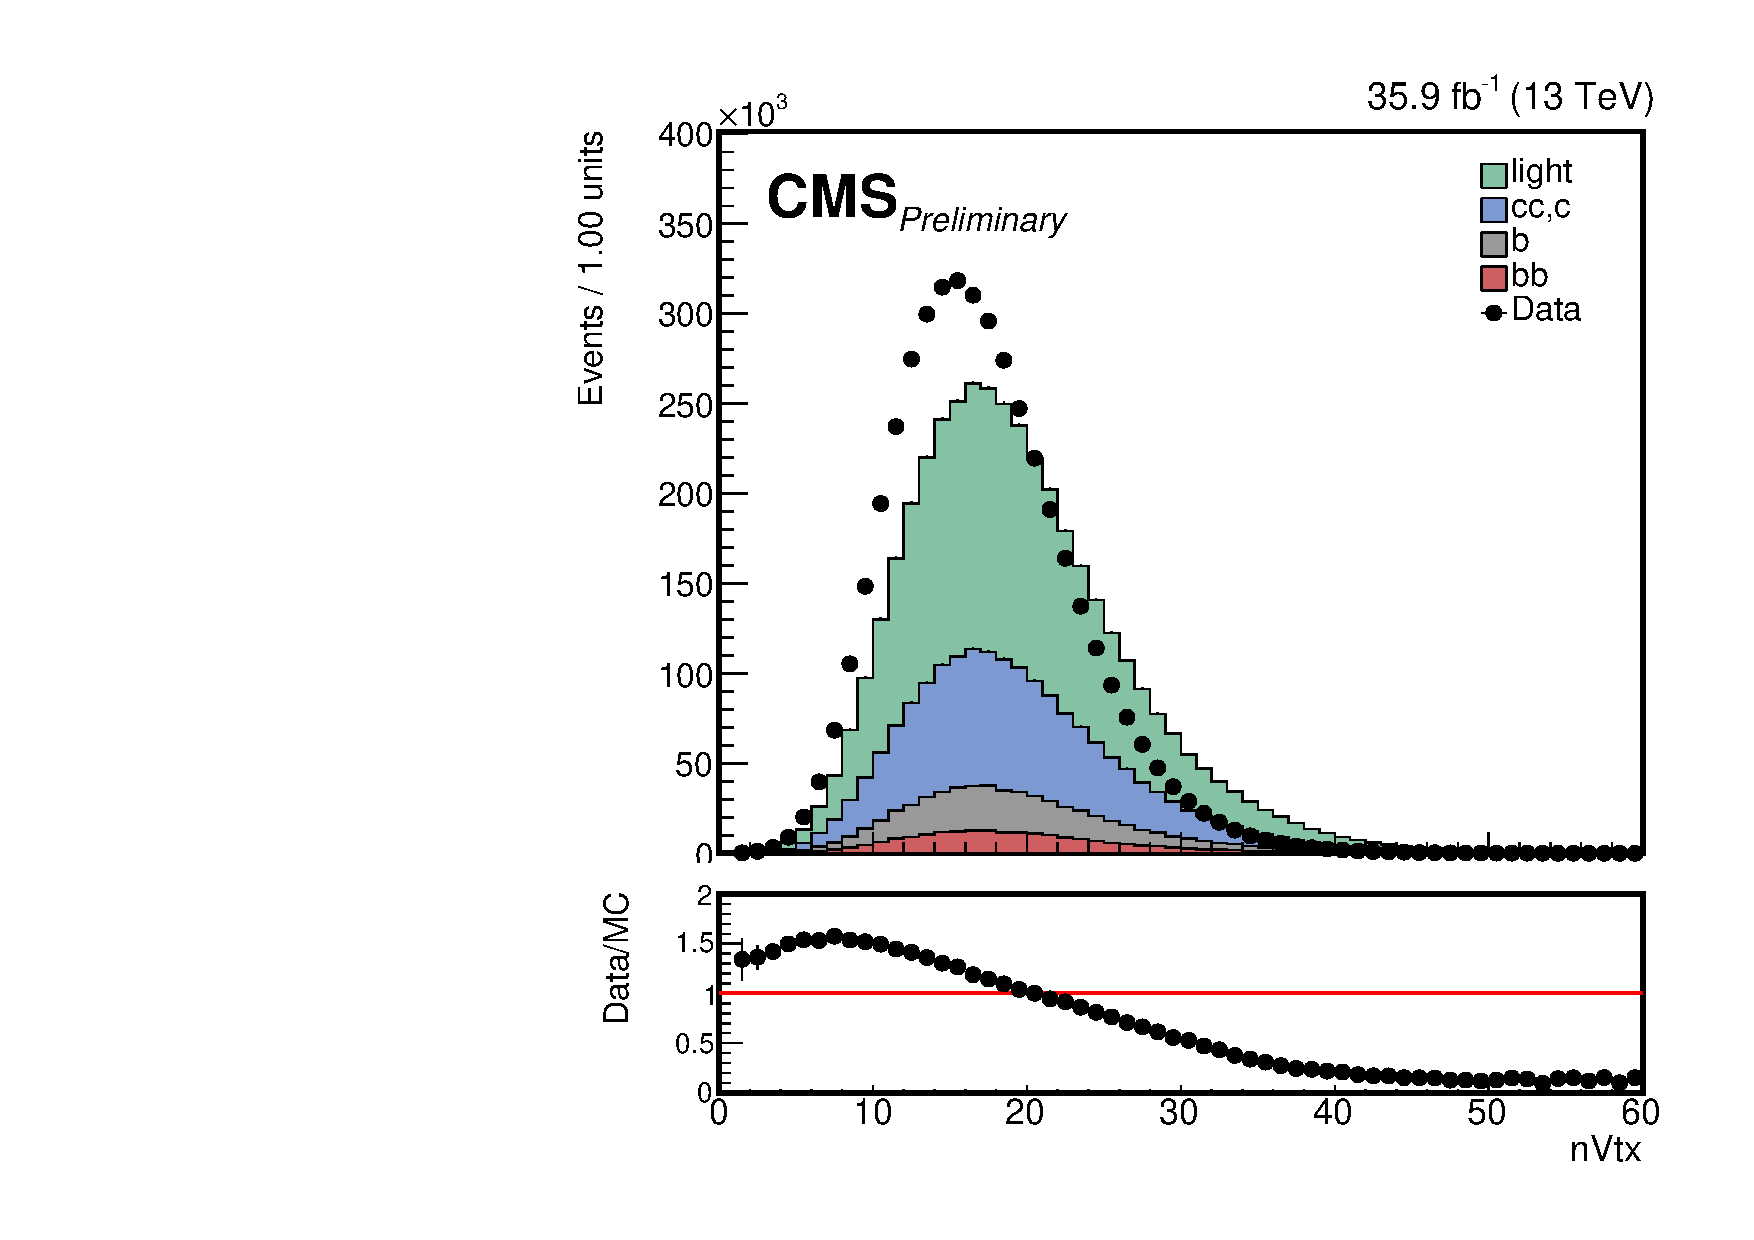
\includegraphics[width=0.5\textwidth]{Figures/dataMC_trig/nVtx.pdf} &
    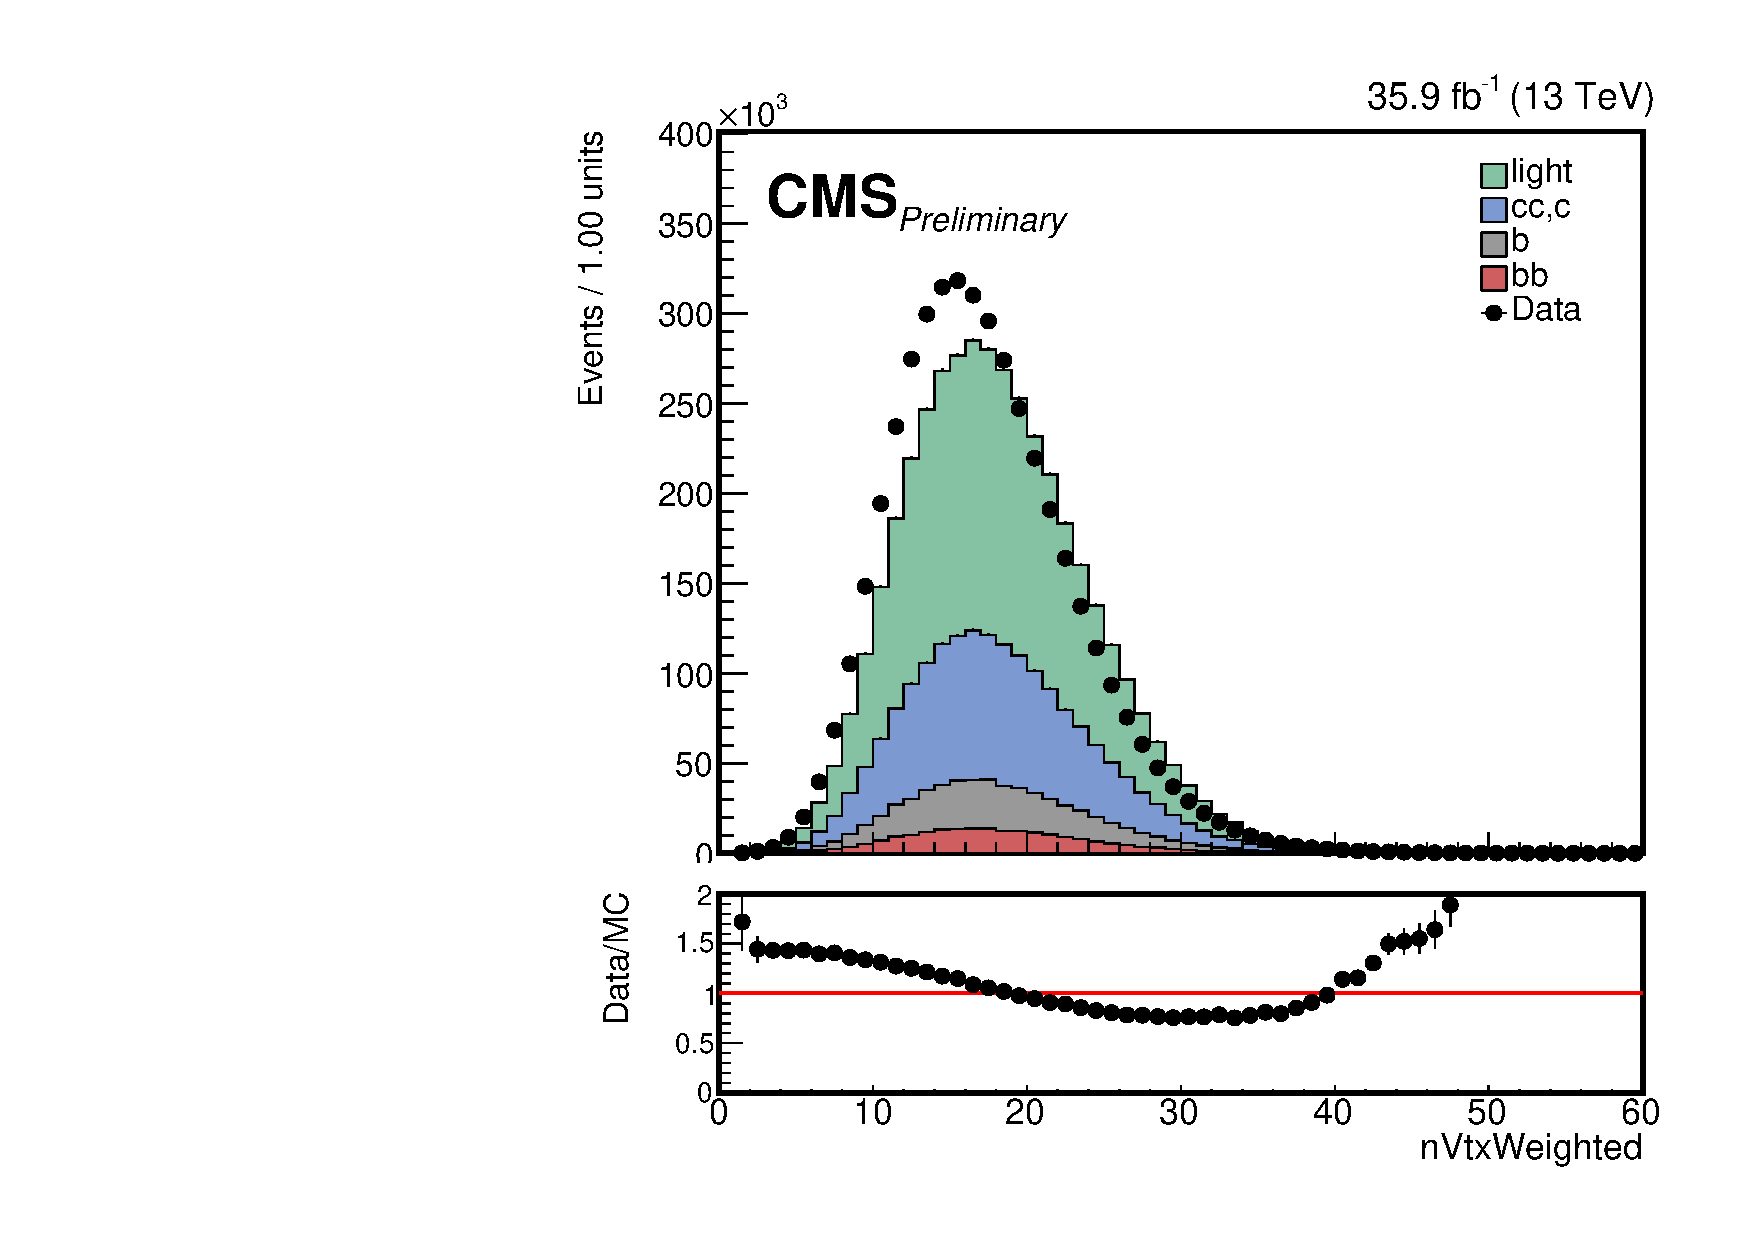
\includegraphics[width=0.5\textwidth]{Figures/dataMC_trig/nVtxWeighted.pdf} \\
    
  \end{tabular}
  \caption{The comparison of data and background of pile-up distribution with (left) and without (right) pile-up re-weighting. Multi-jet events are seperated into four categories summarized in the table 3.10.}
\end{figure}
\begin{figure}[t]
  \centering
  \begin{tabular}{cc}
    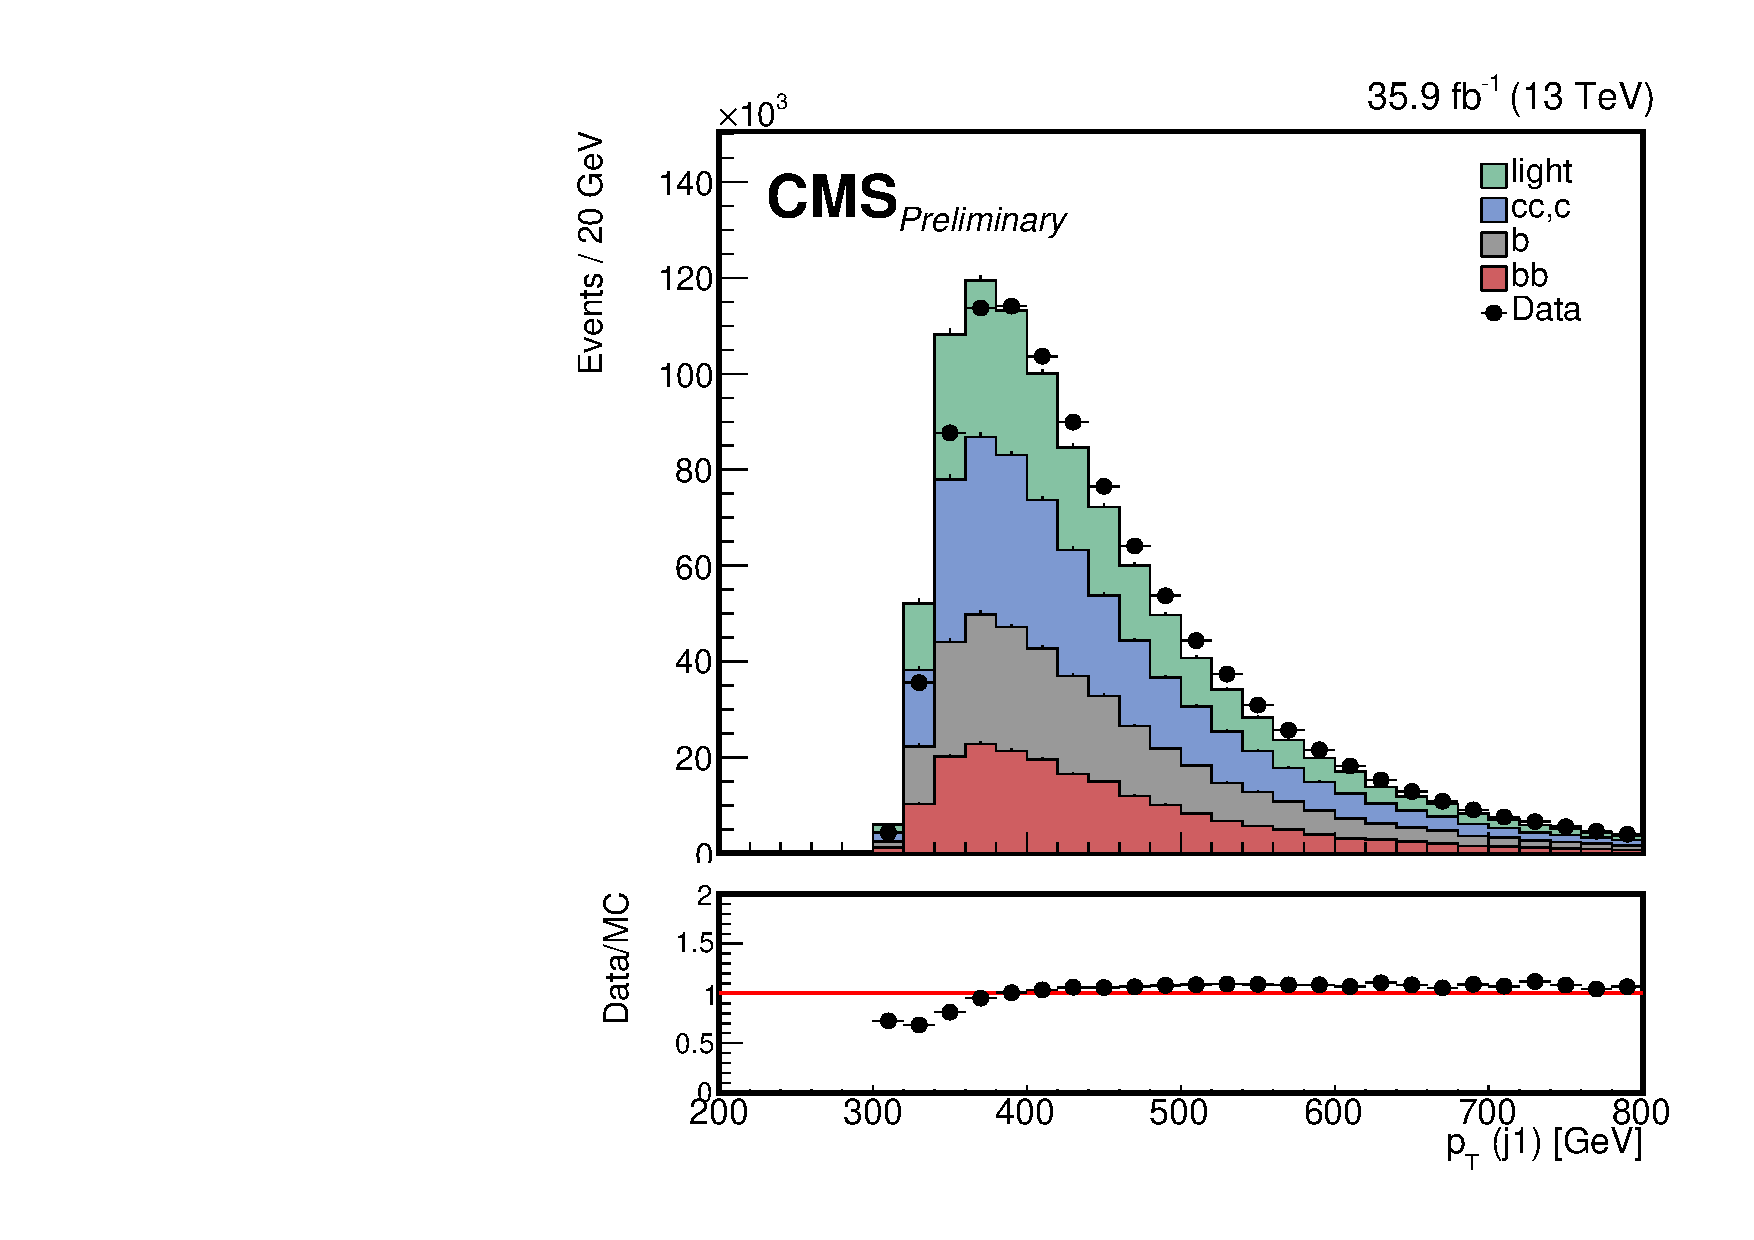
\includegraphics[width=0.5\textwidth]{Figures/dataMC_trig_antiDBT/pt_j0.pdf} &
    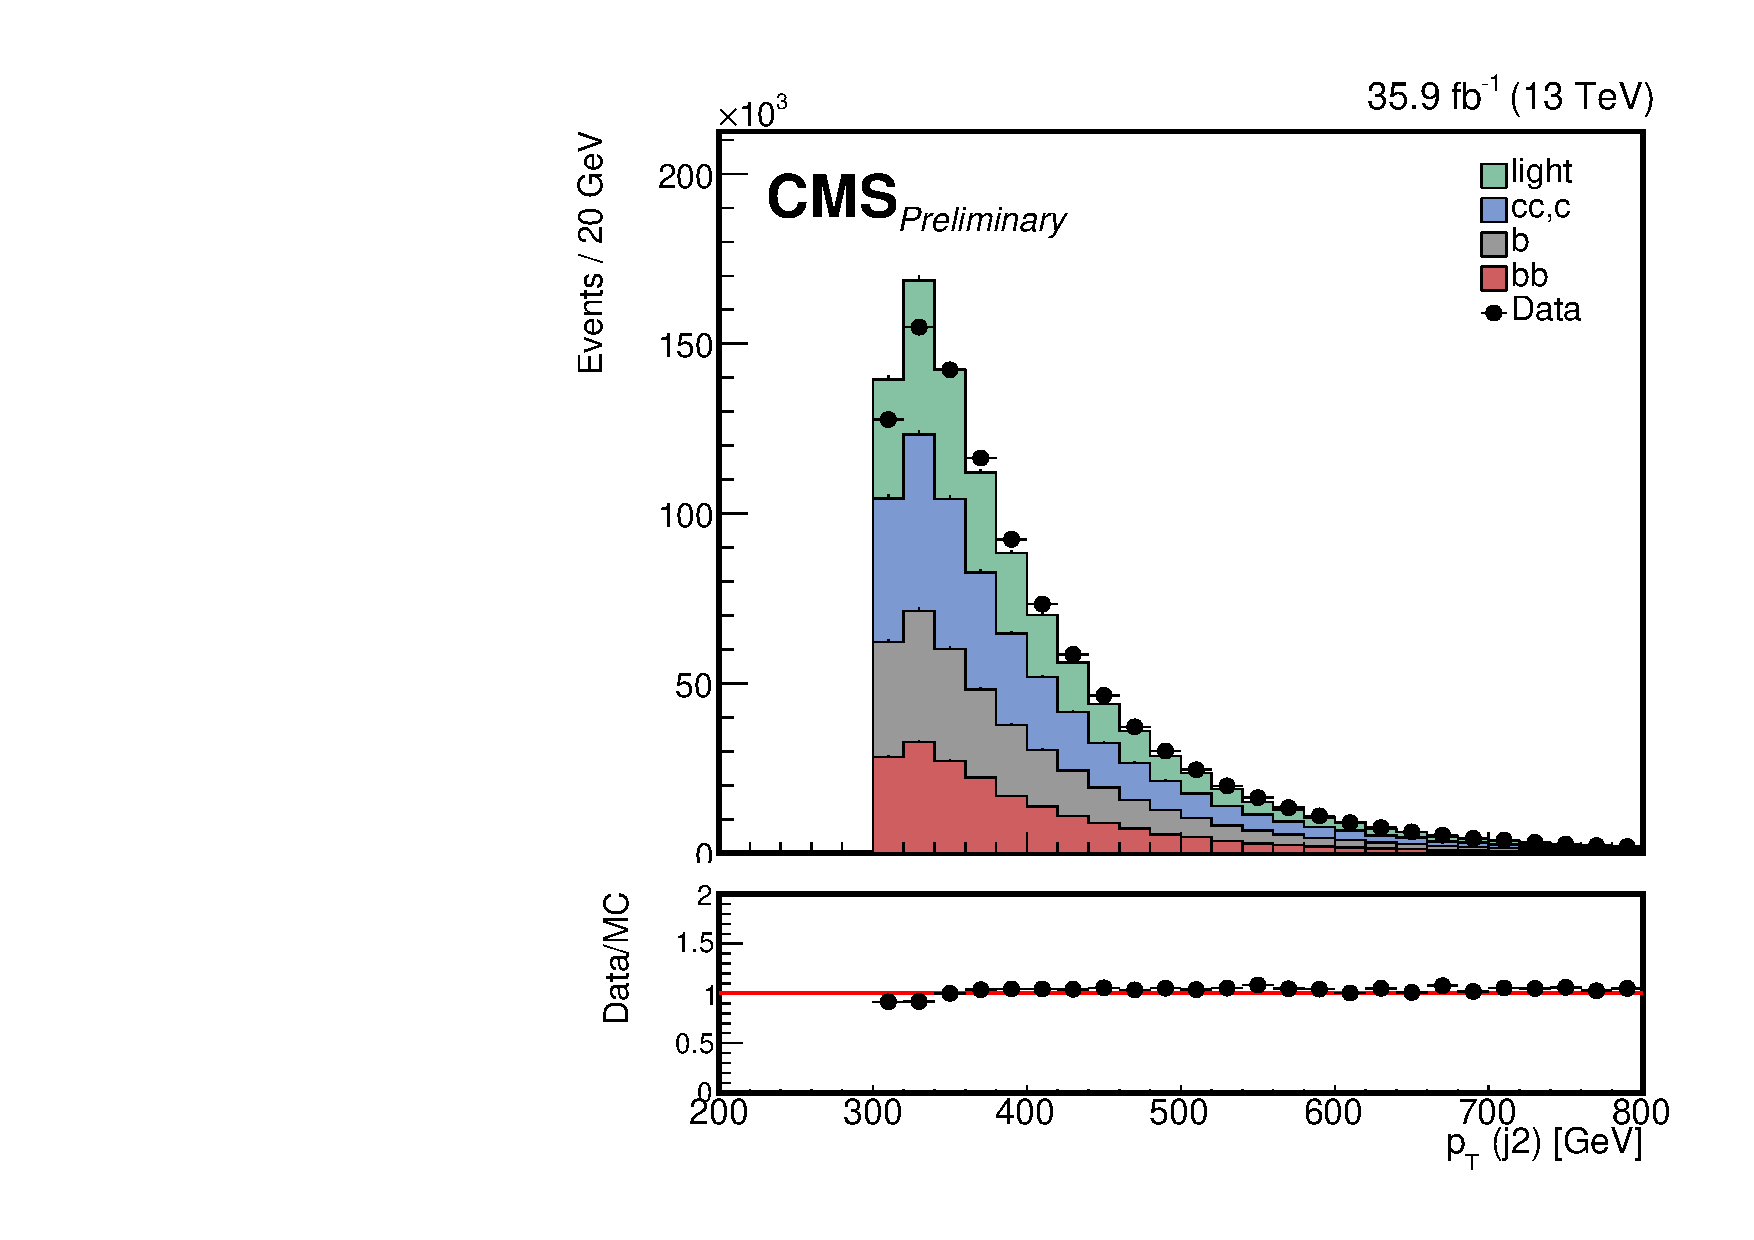
\includegraphics[width=0.5\textwidth]{Figures/dataMC_trig_antiDBT/pt_j1.pdf} \\
     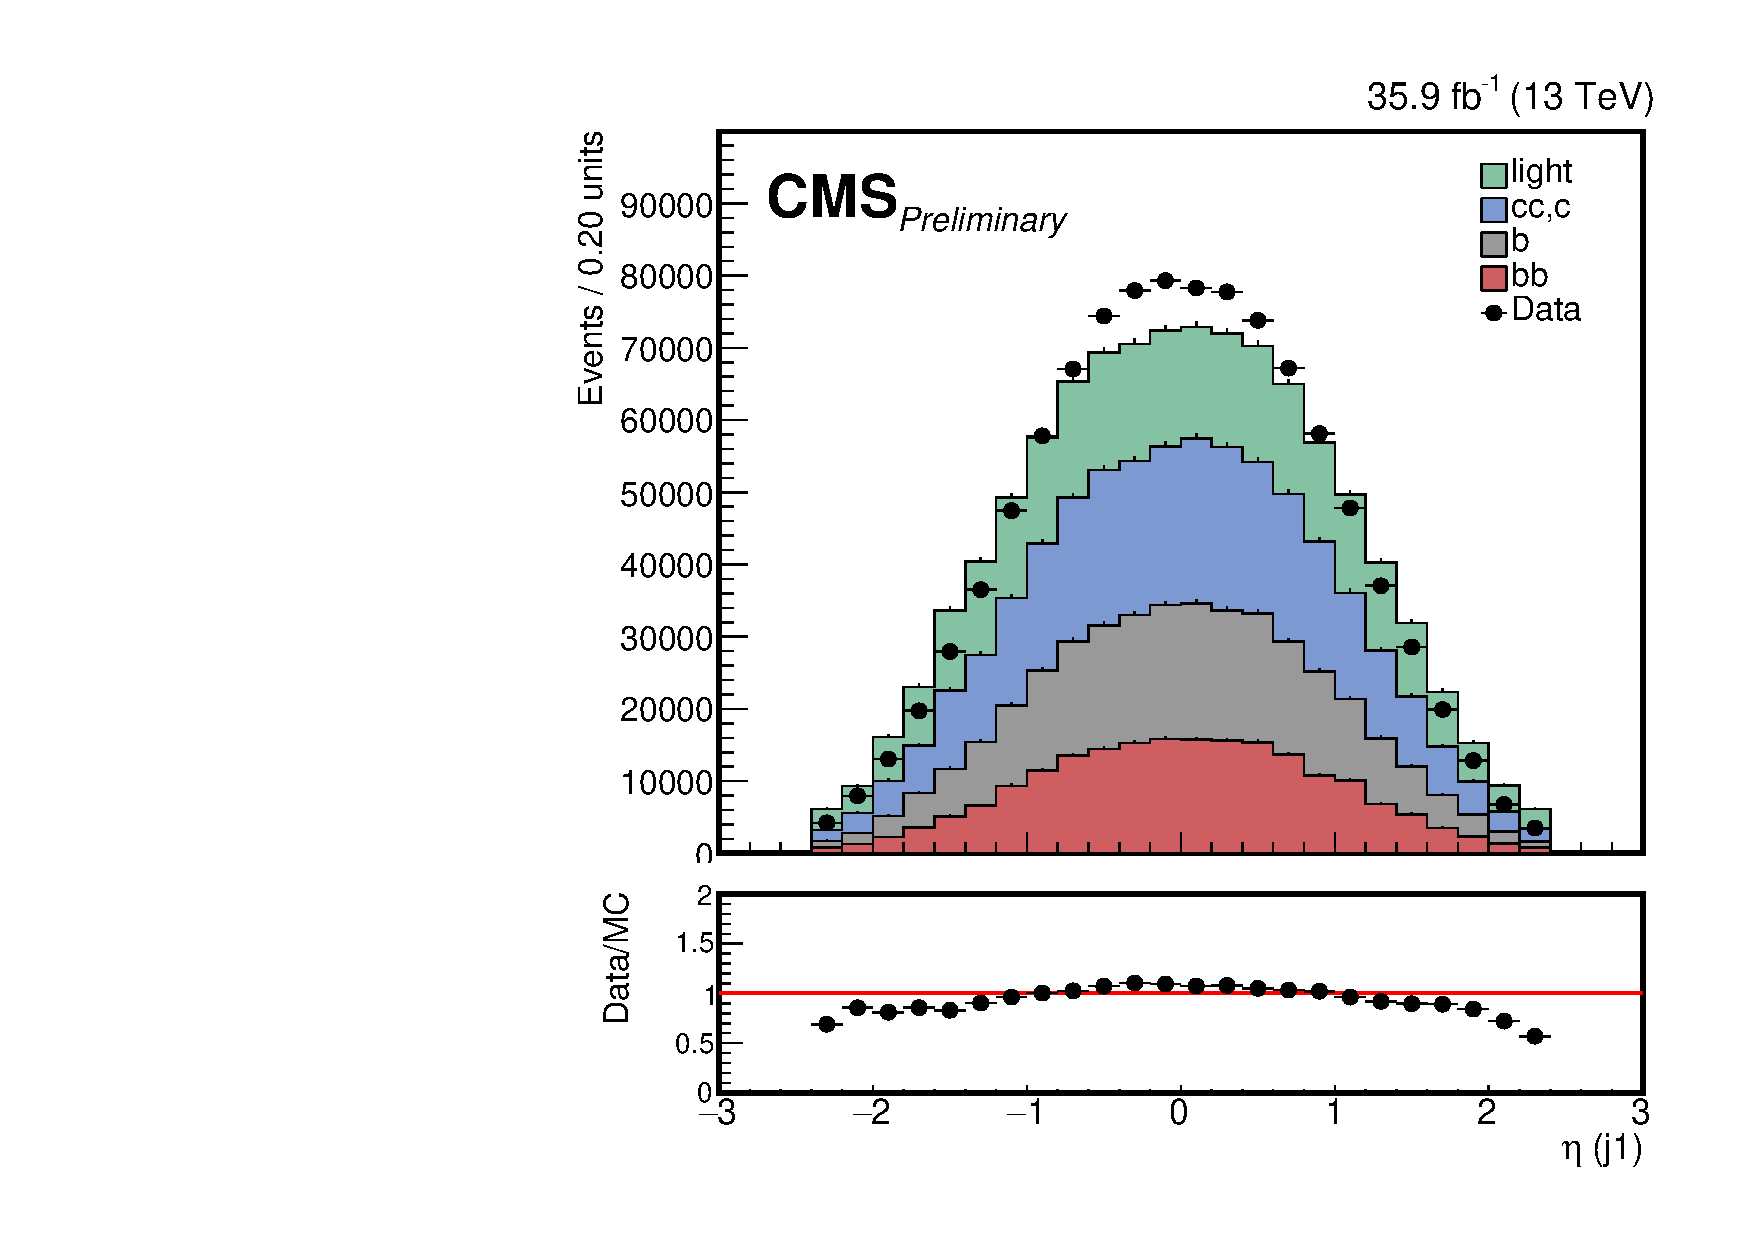
\includegraphics[width=0.5\textwidth]{Figures/dataMC_trig_antiDBT/eta_j0.pdf} &
    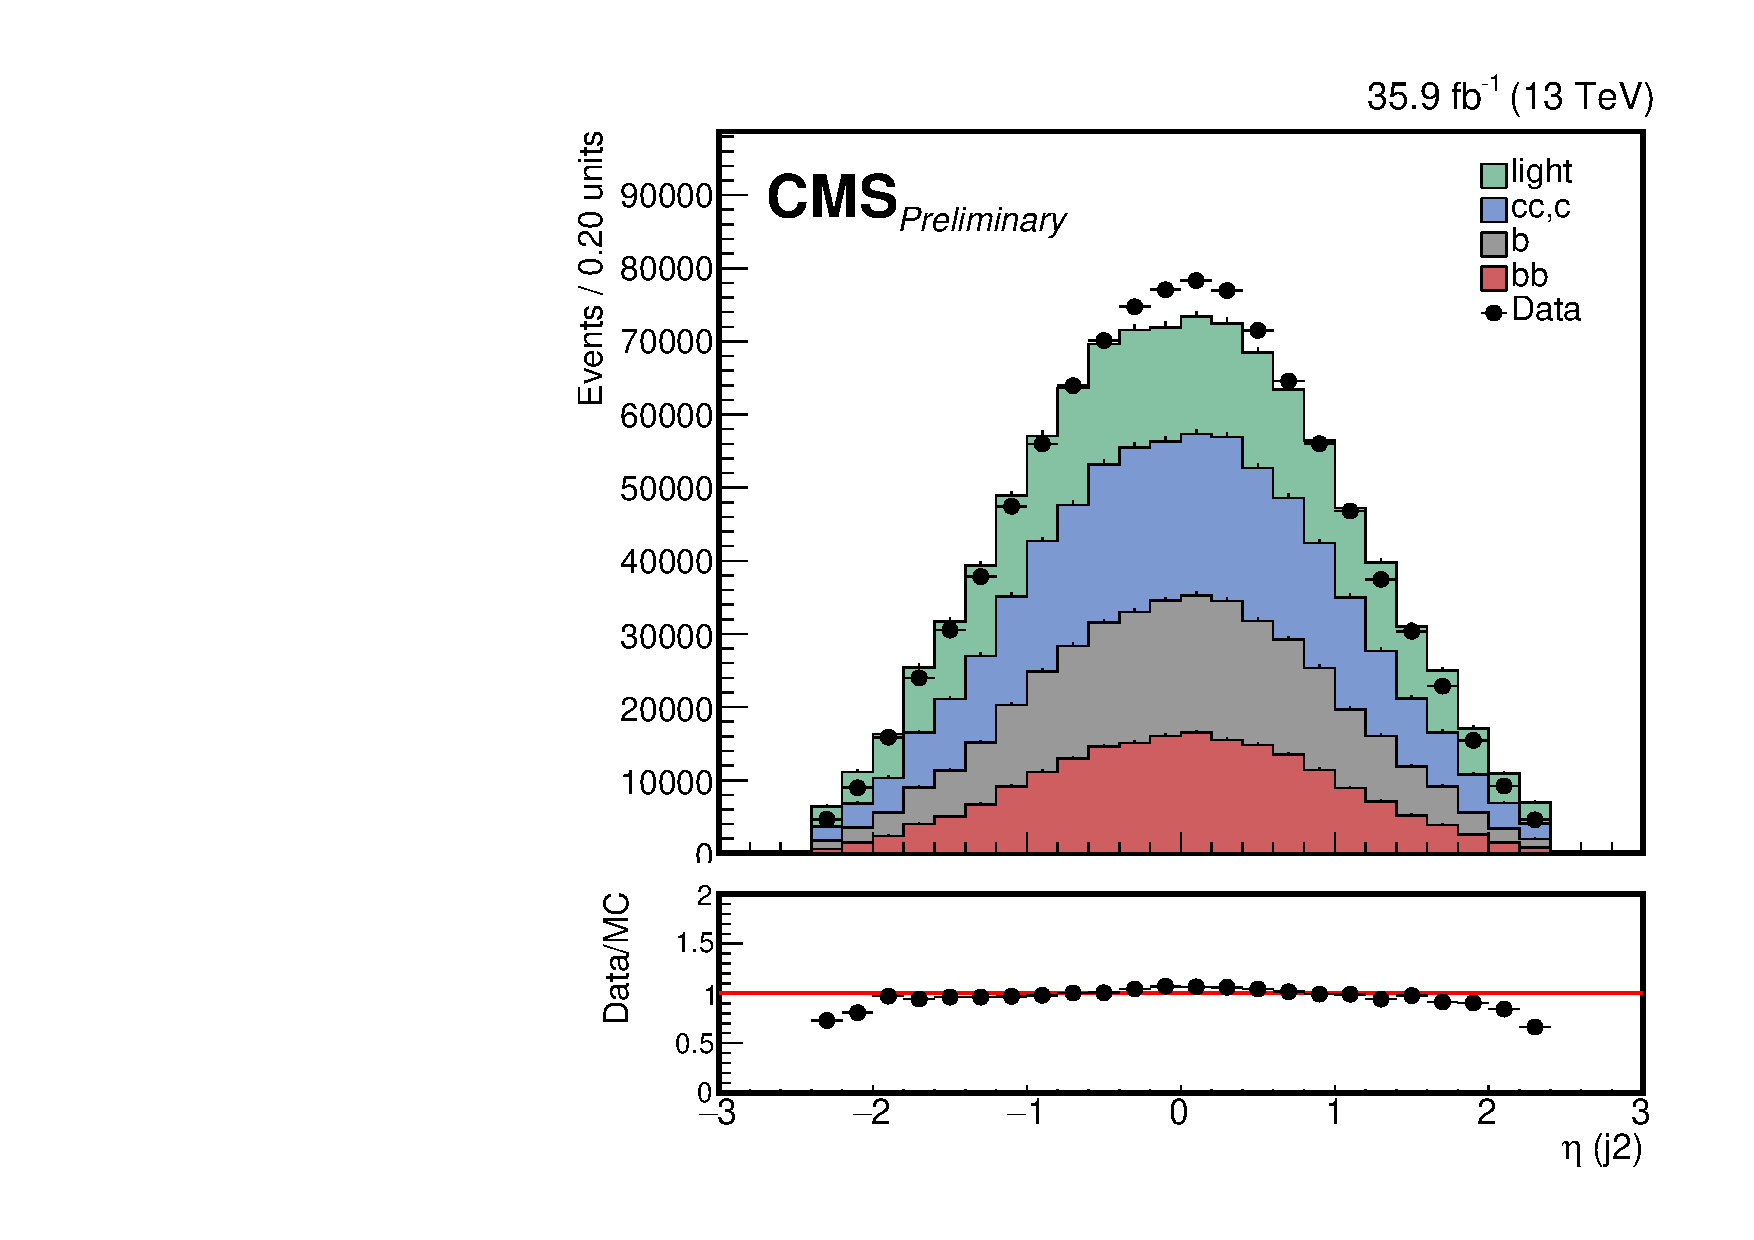
\includegraphics[width=0.5\textwidth]{Figures/dataMC_trig_antiDBT/eta_j1.pdf} \\
     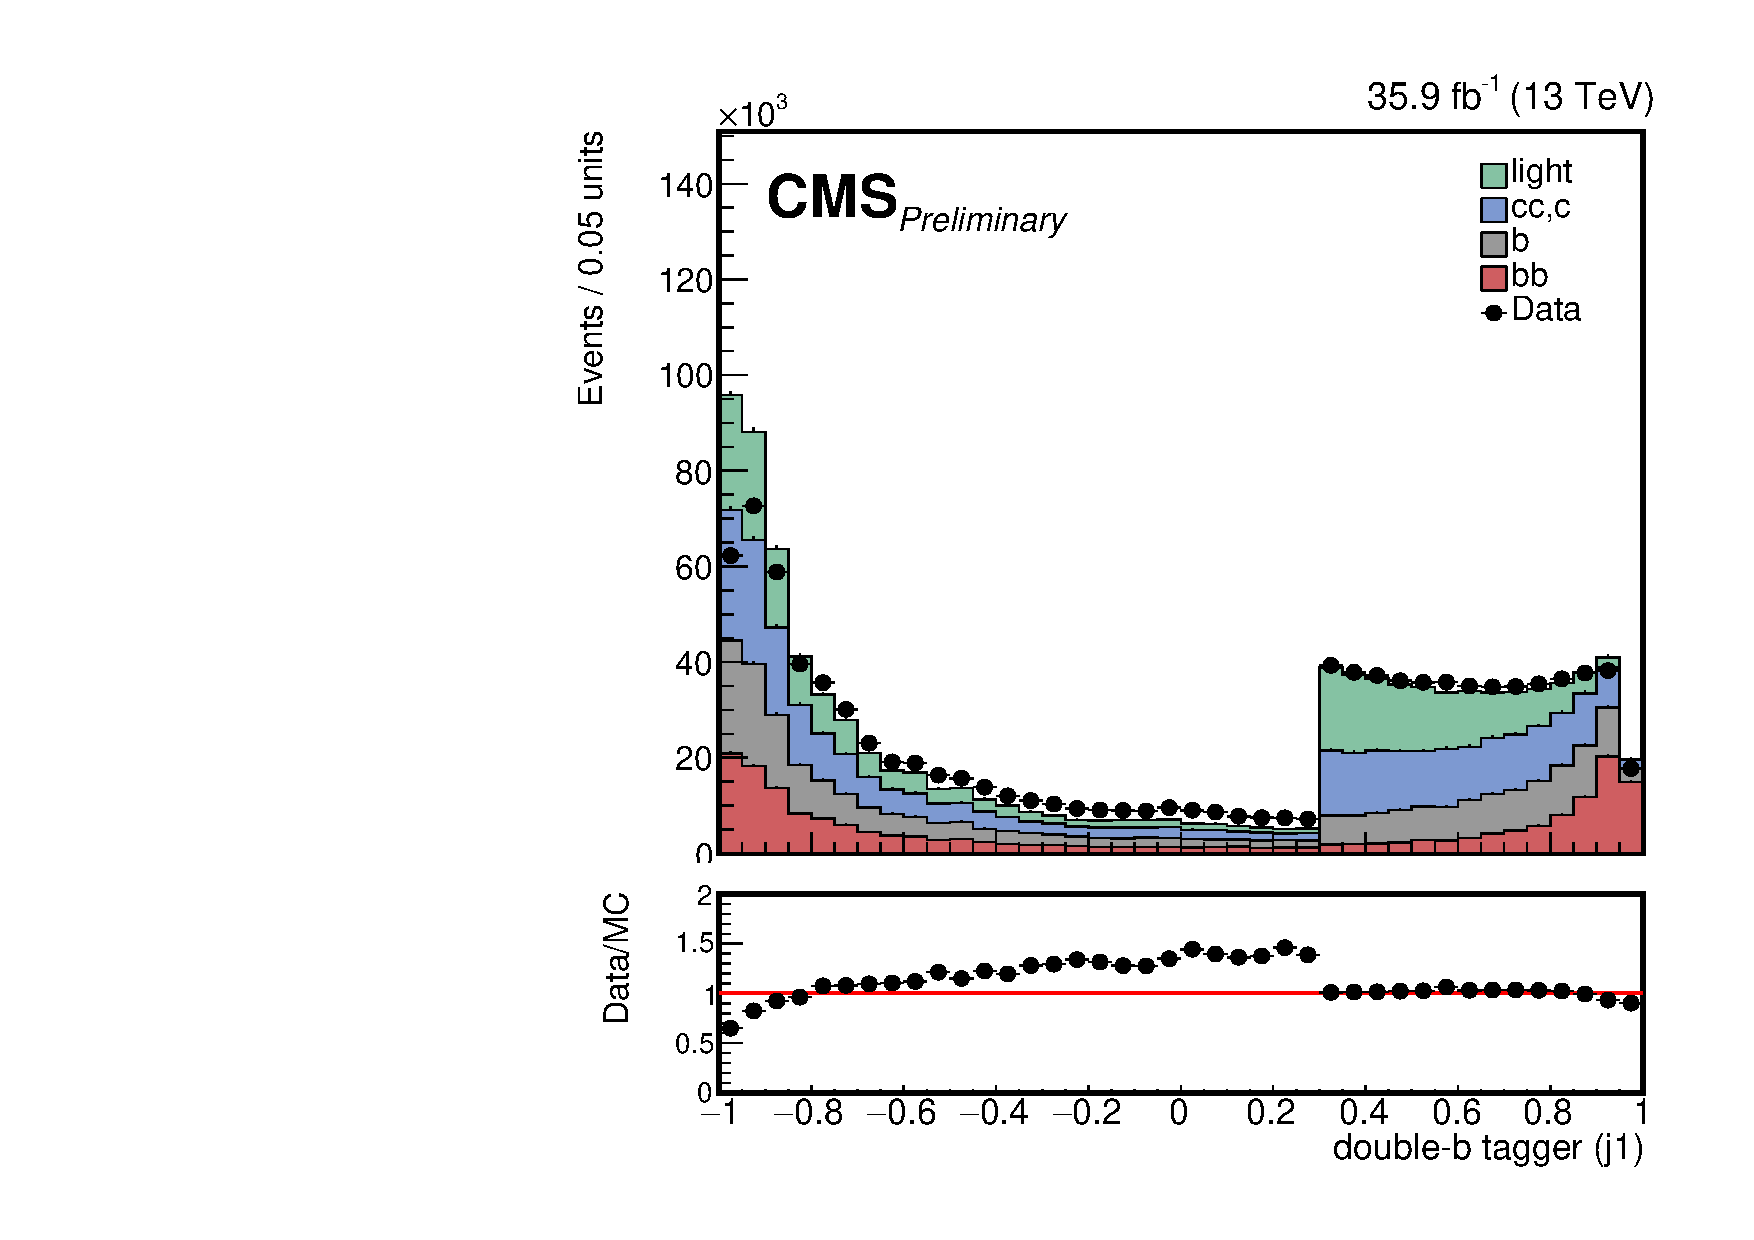
\includegraphics[width=0.5\textwidth]{Figures/dataMC_trig_antiDBT/doubleSV_j0.pdf} &
    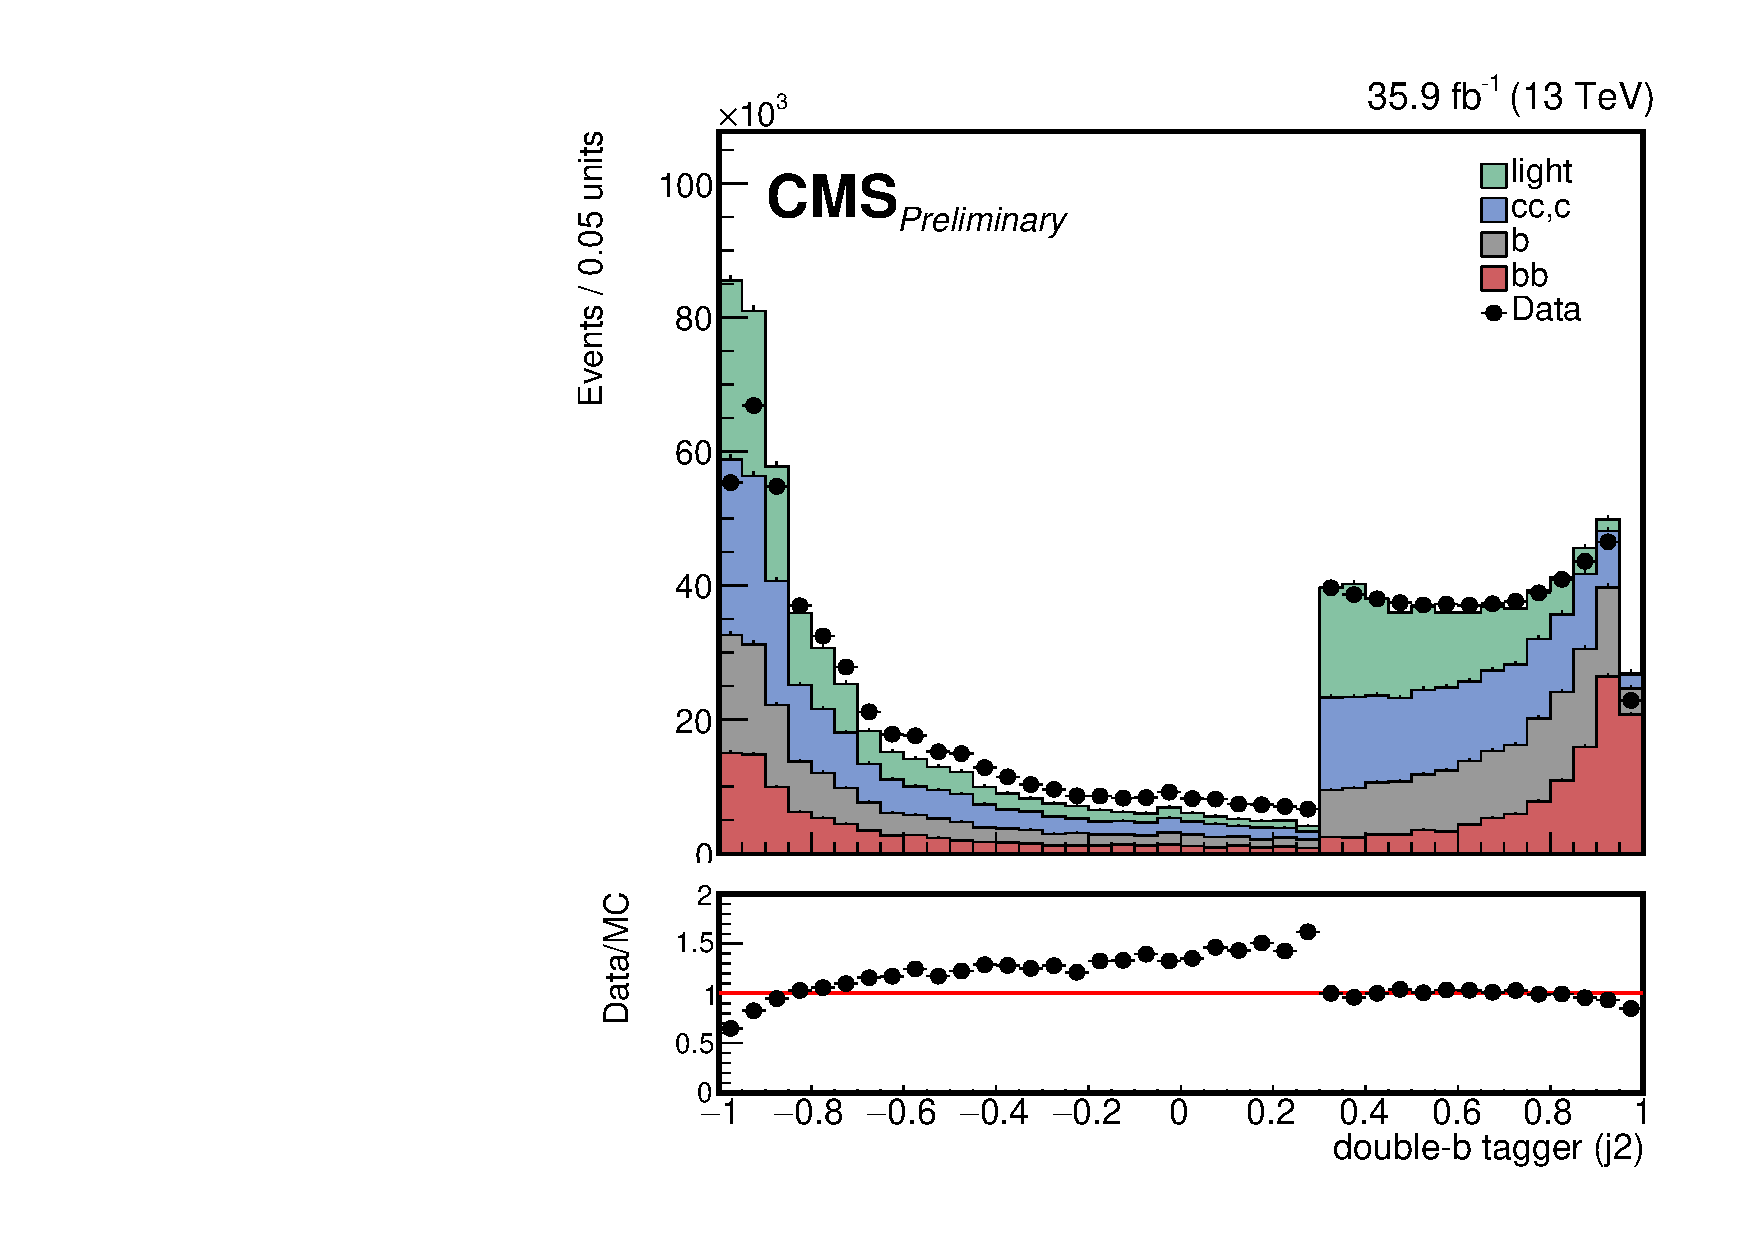
\includegraphics[width=0.5\textwidth]{Figures/dataMC_trig_antiDBT/doubleSV_j1.pdf} \\
  \end{tabular}
  \caption{The comparison of data and background in inverse double-b region. Multi-jet events are seperated into four categories summarized in the table 3.10. From top to buttom are the comparison of $p_{T}$, $\eta $, and double-b tagger of leading (left) and next leading (right) AK8 jet.}
  \label{fig:hvt_brs}
\end{figure}
\begin{figure}[t]
  \centering
  \begin{tabular}{cc}
    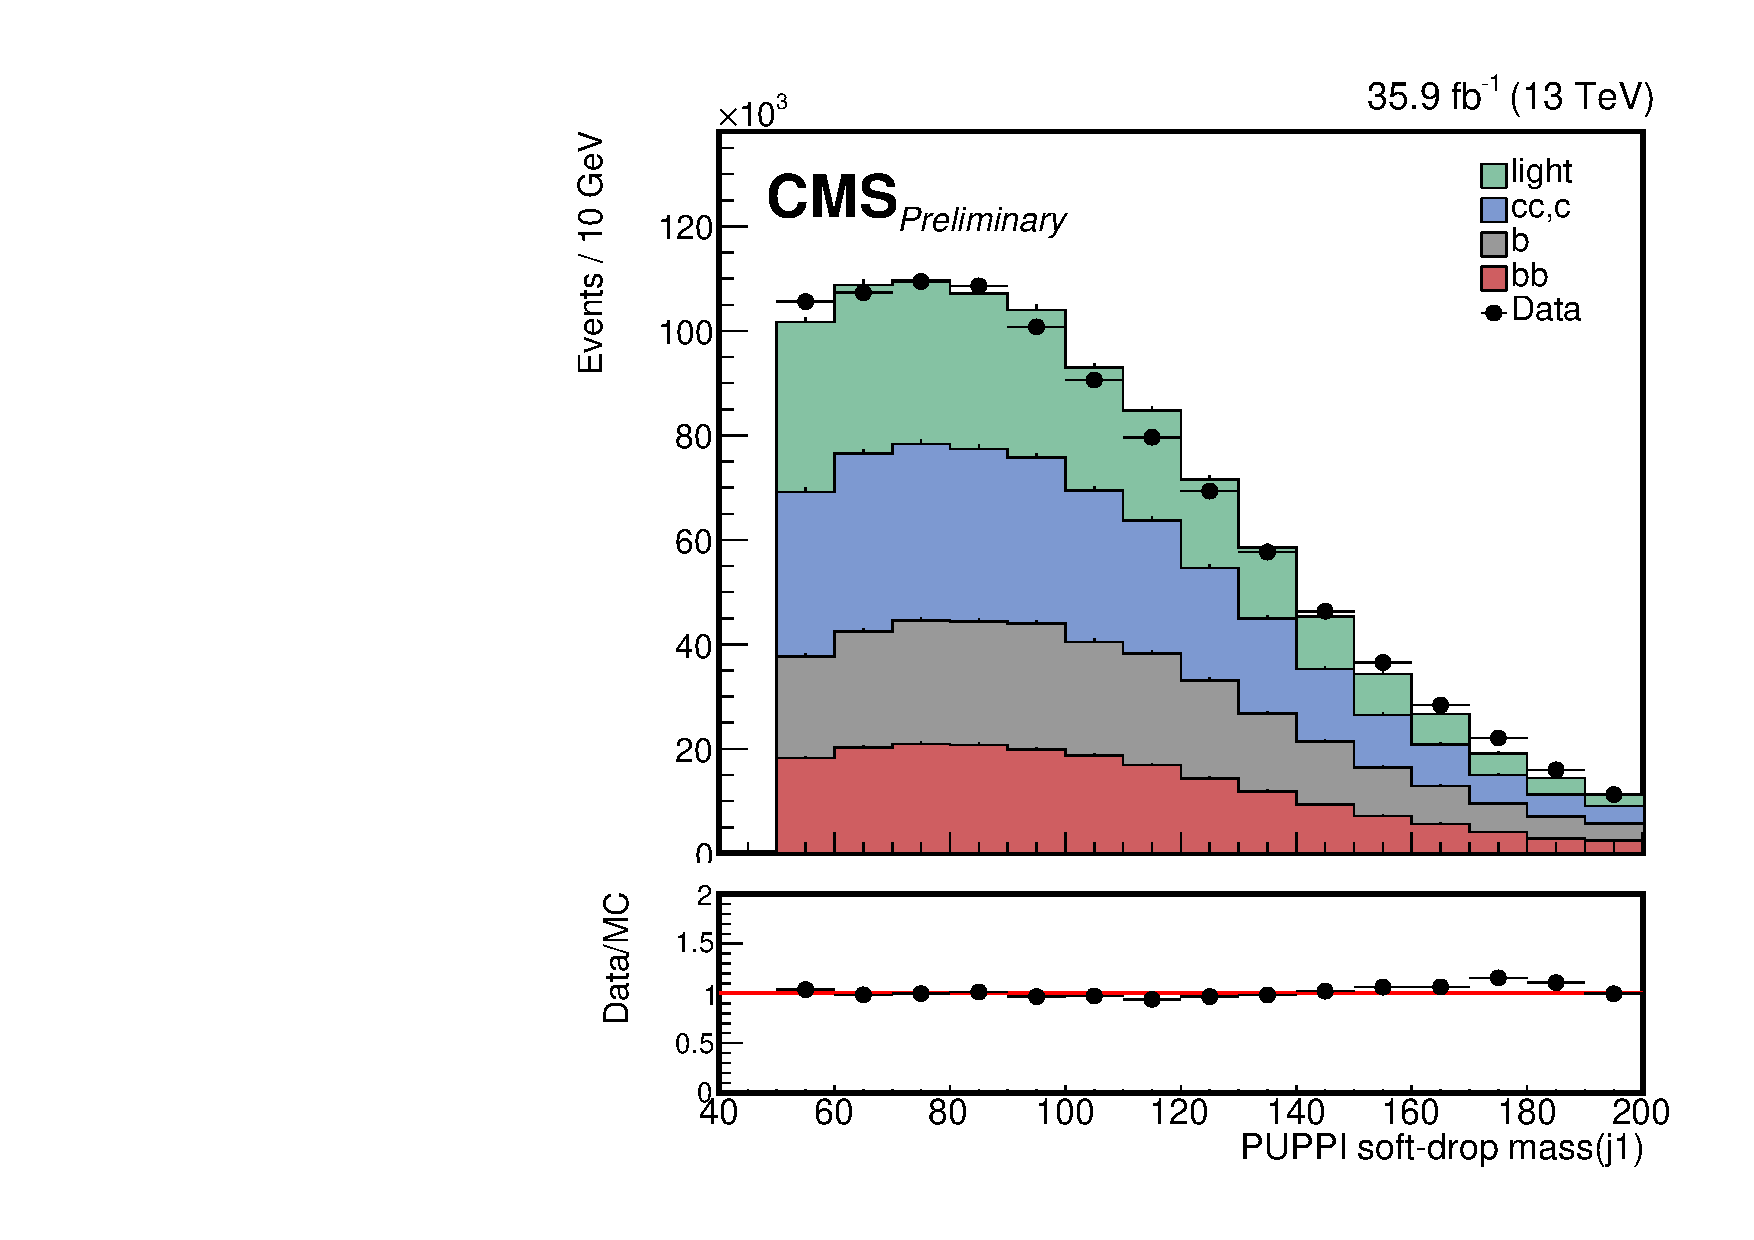
\includegraphics[width=0.5\textwidth]{Figures/dataMC_trig_antiDBT/puppiSDMassThea_j0.pdf} &
    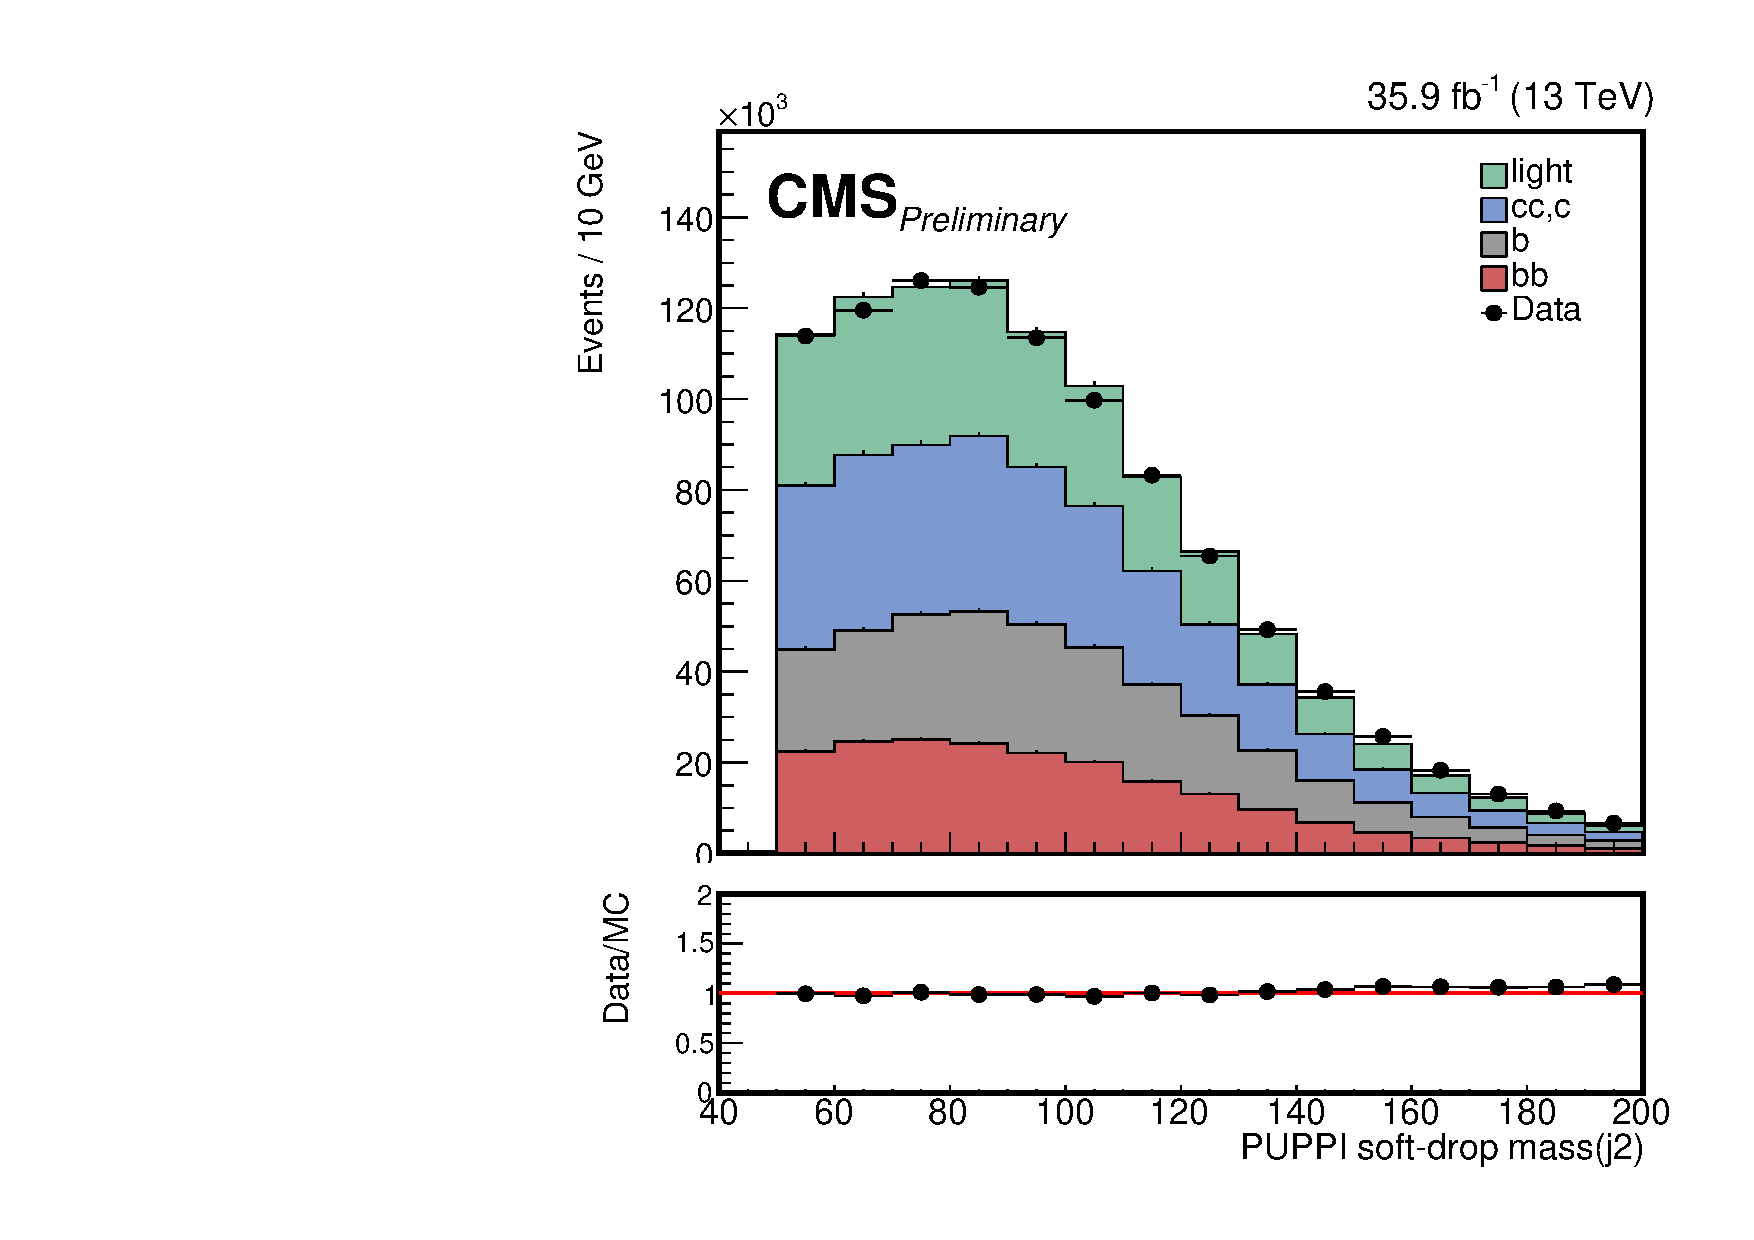
\includegraphics[width=0.5\textwidth]{Figures/dataMC_trig_antiDBT/puppiSDMassThea_j1.pdf} \\
     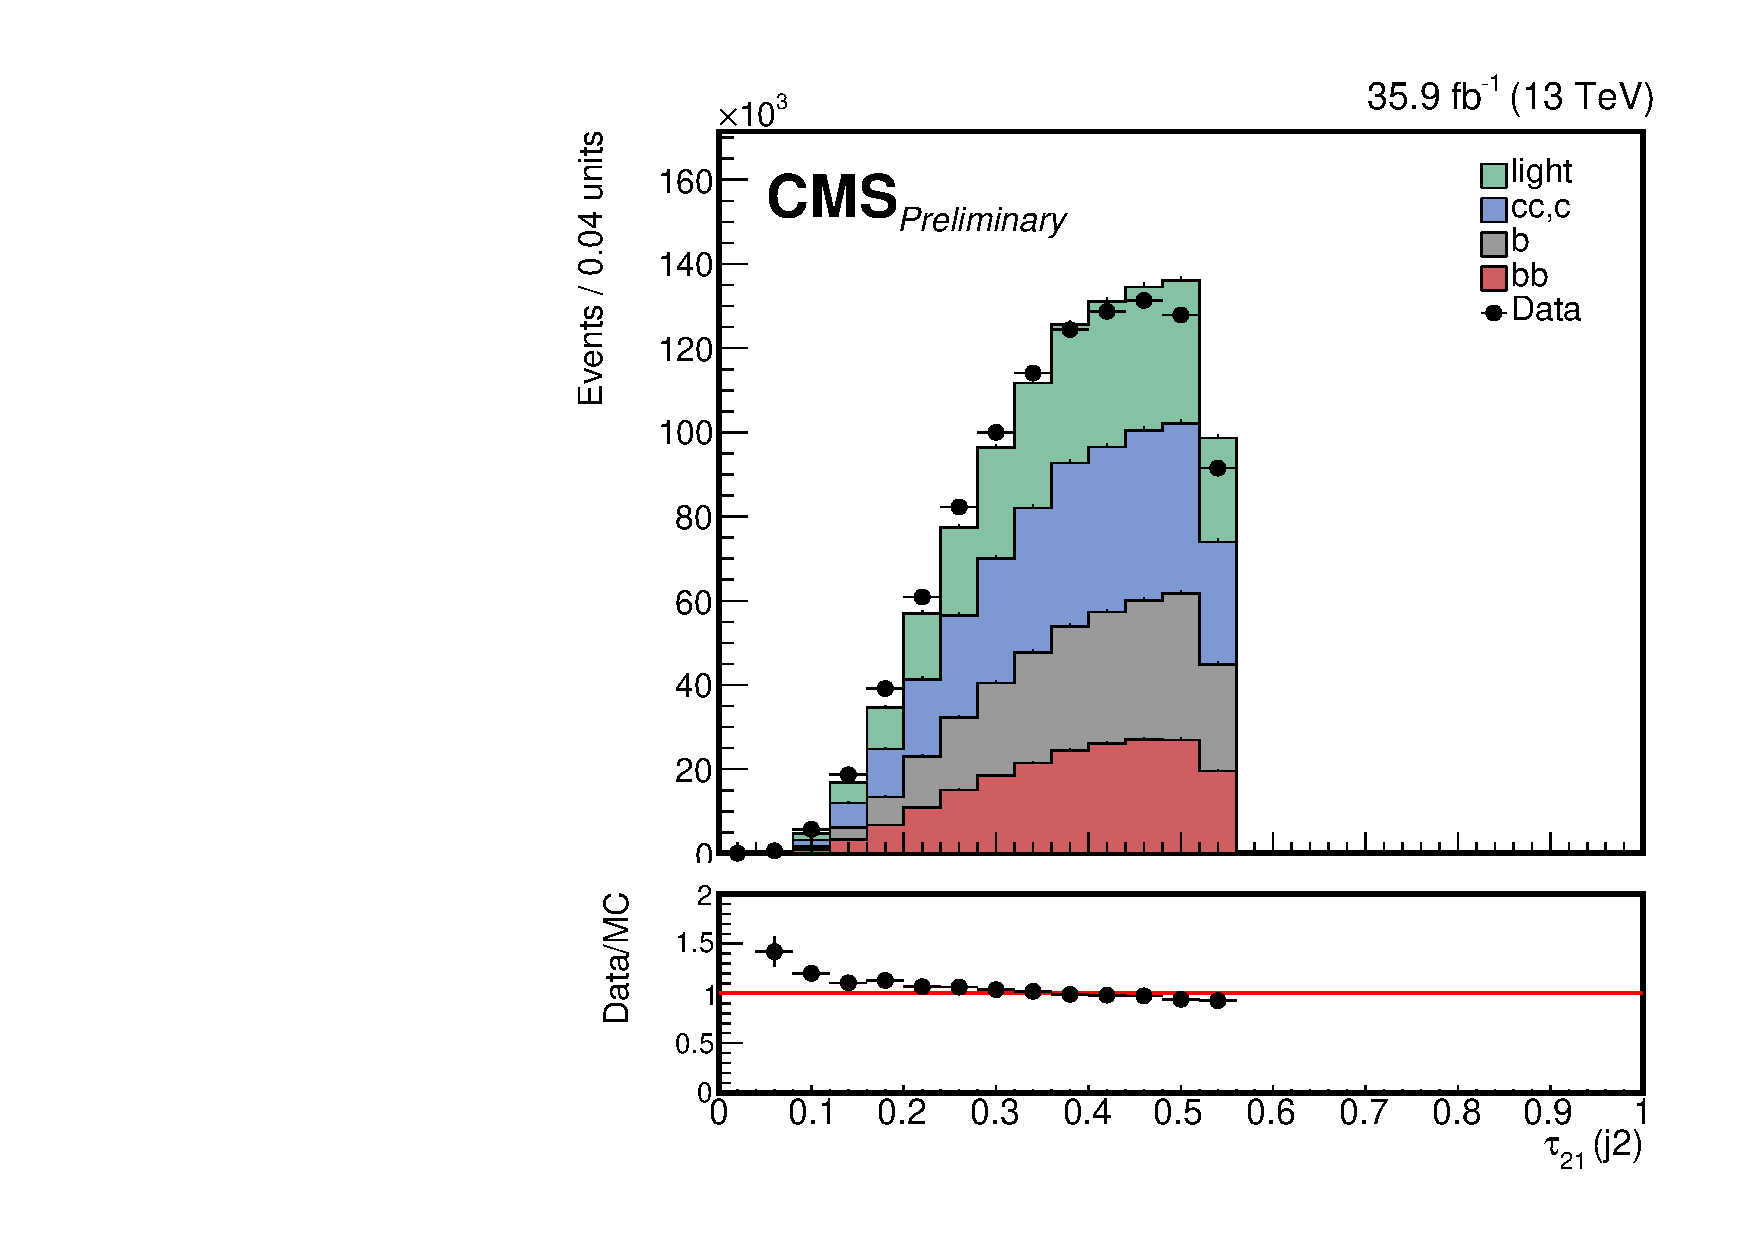
\includegraphics[width=0.5\textwidth]{Figures/dataMC_trig_antiDBT/puppiTau21_j0.pdf} &
    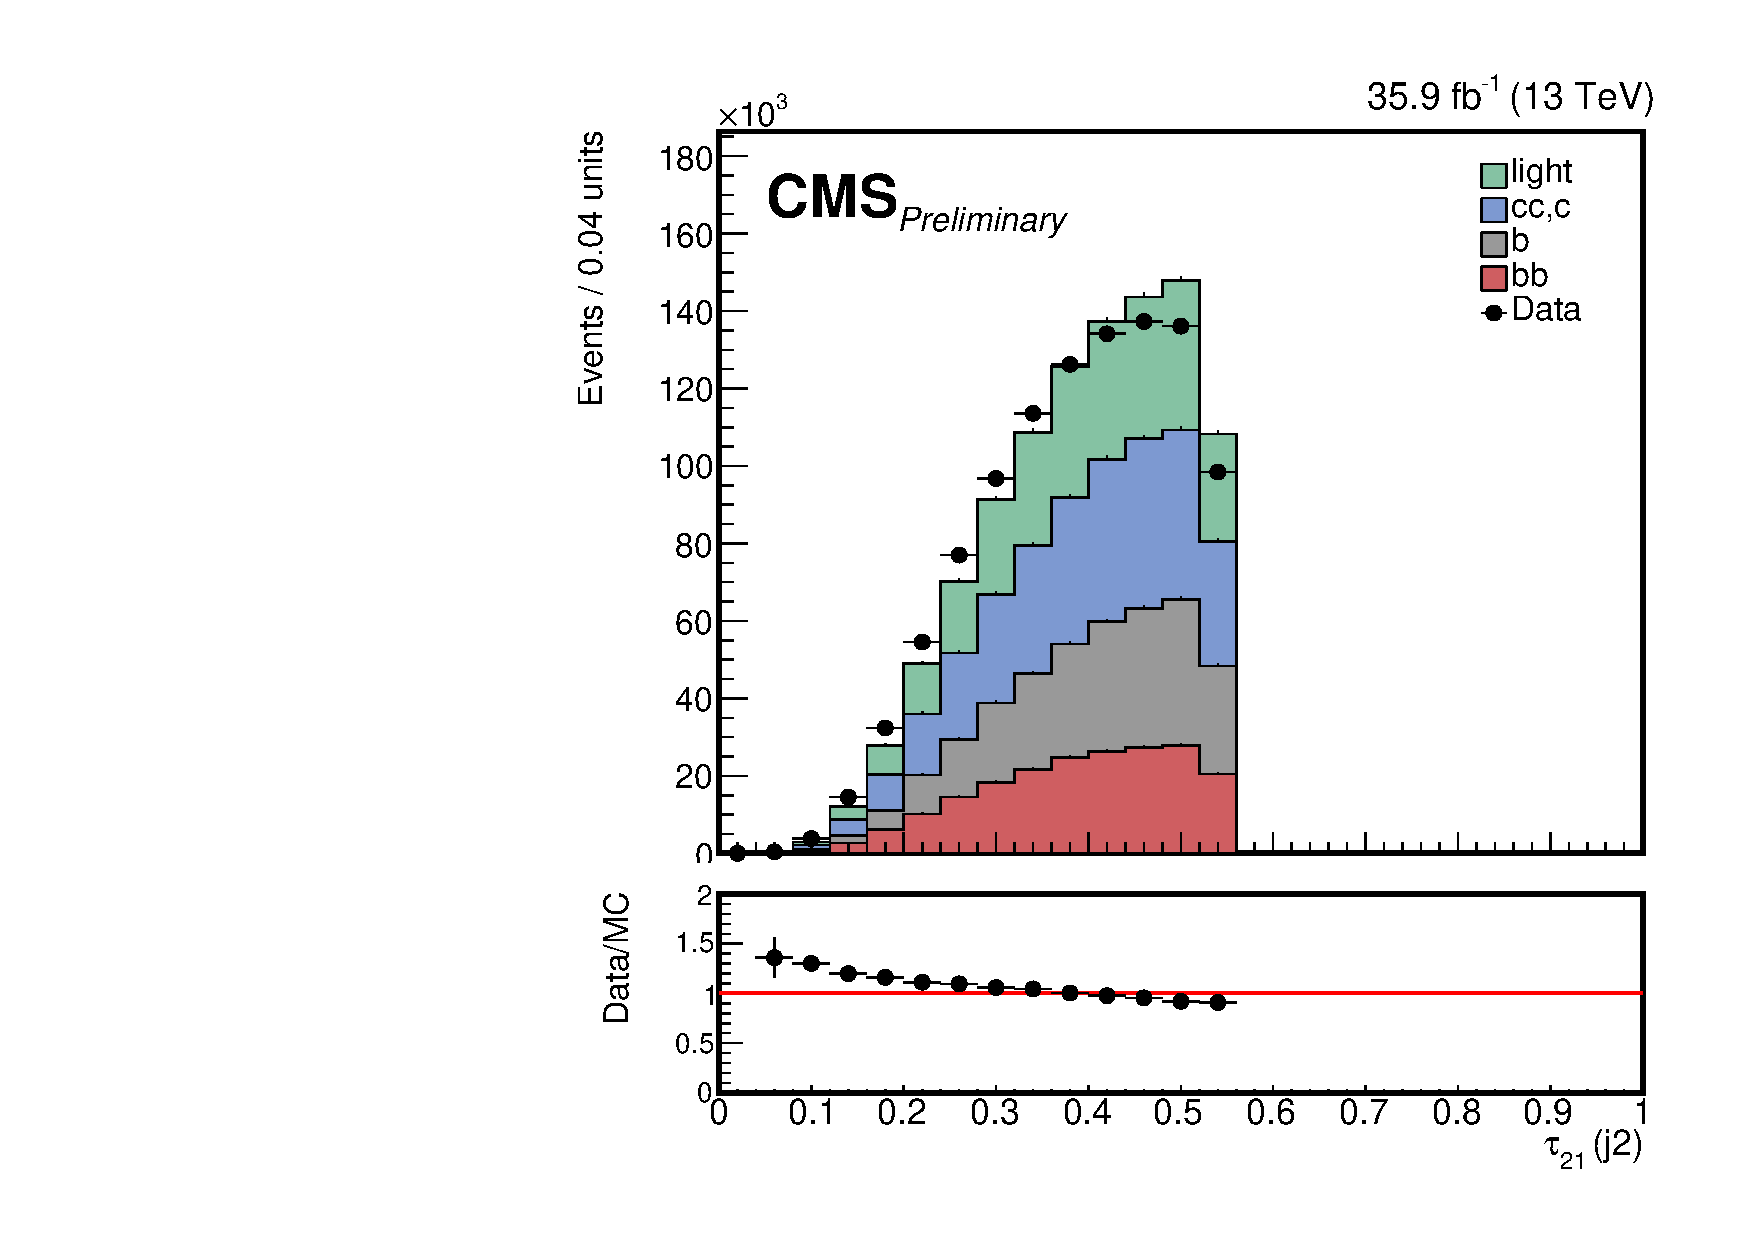
\includegraphics[width=0.5\textwidth]{Figures/dataMC_trig_antiDBT/puppiTau21_j1.pdf} \\
     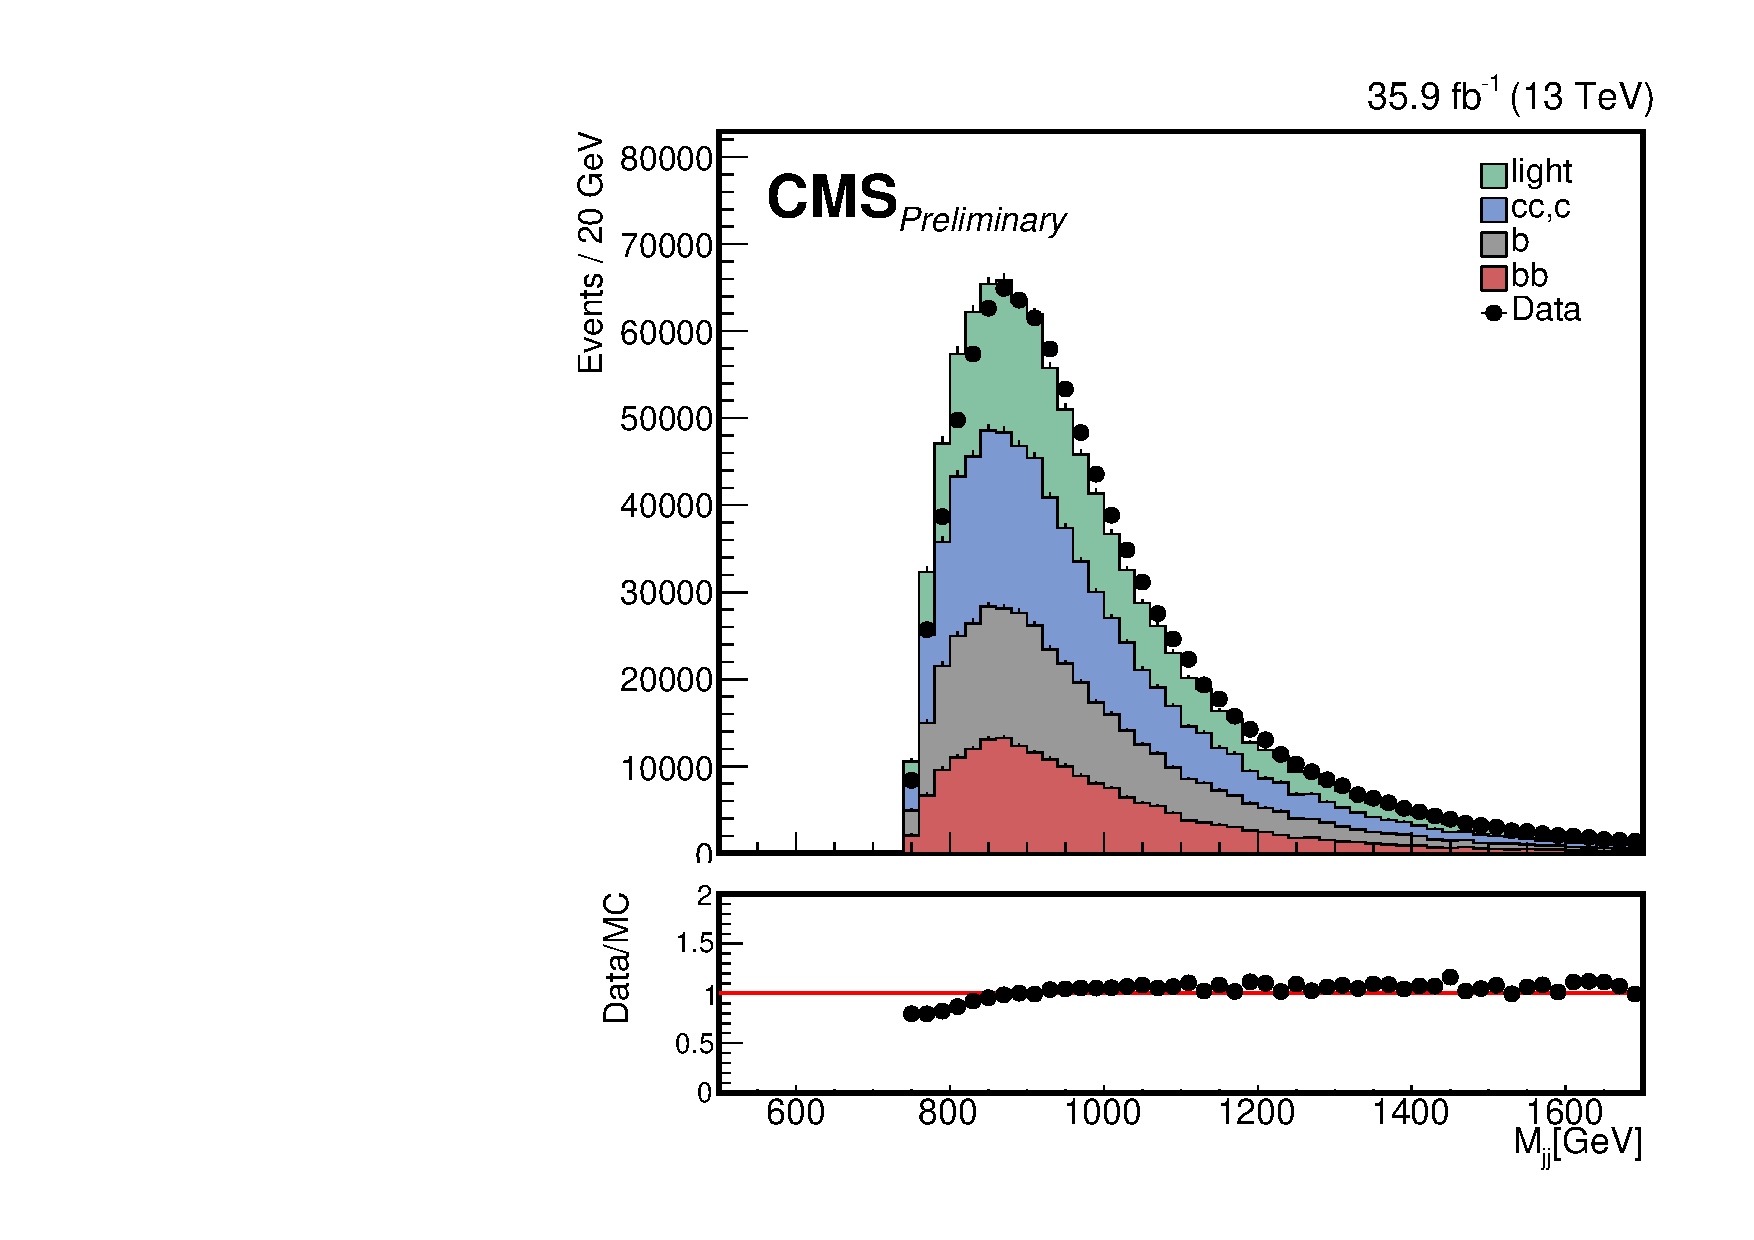
\includegraphics[width=0.5\textwidth]{Figures/dataMC_trig_antiDBT/totalMassRed.pdf} &
    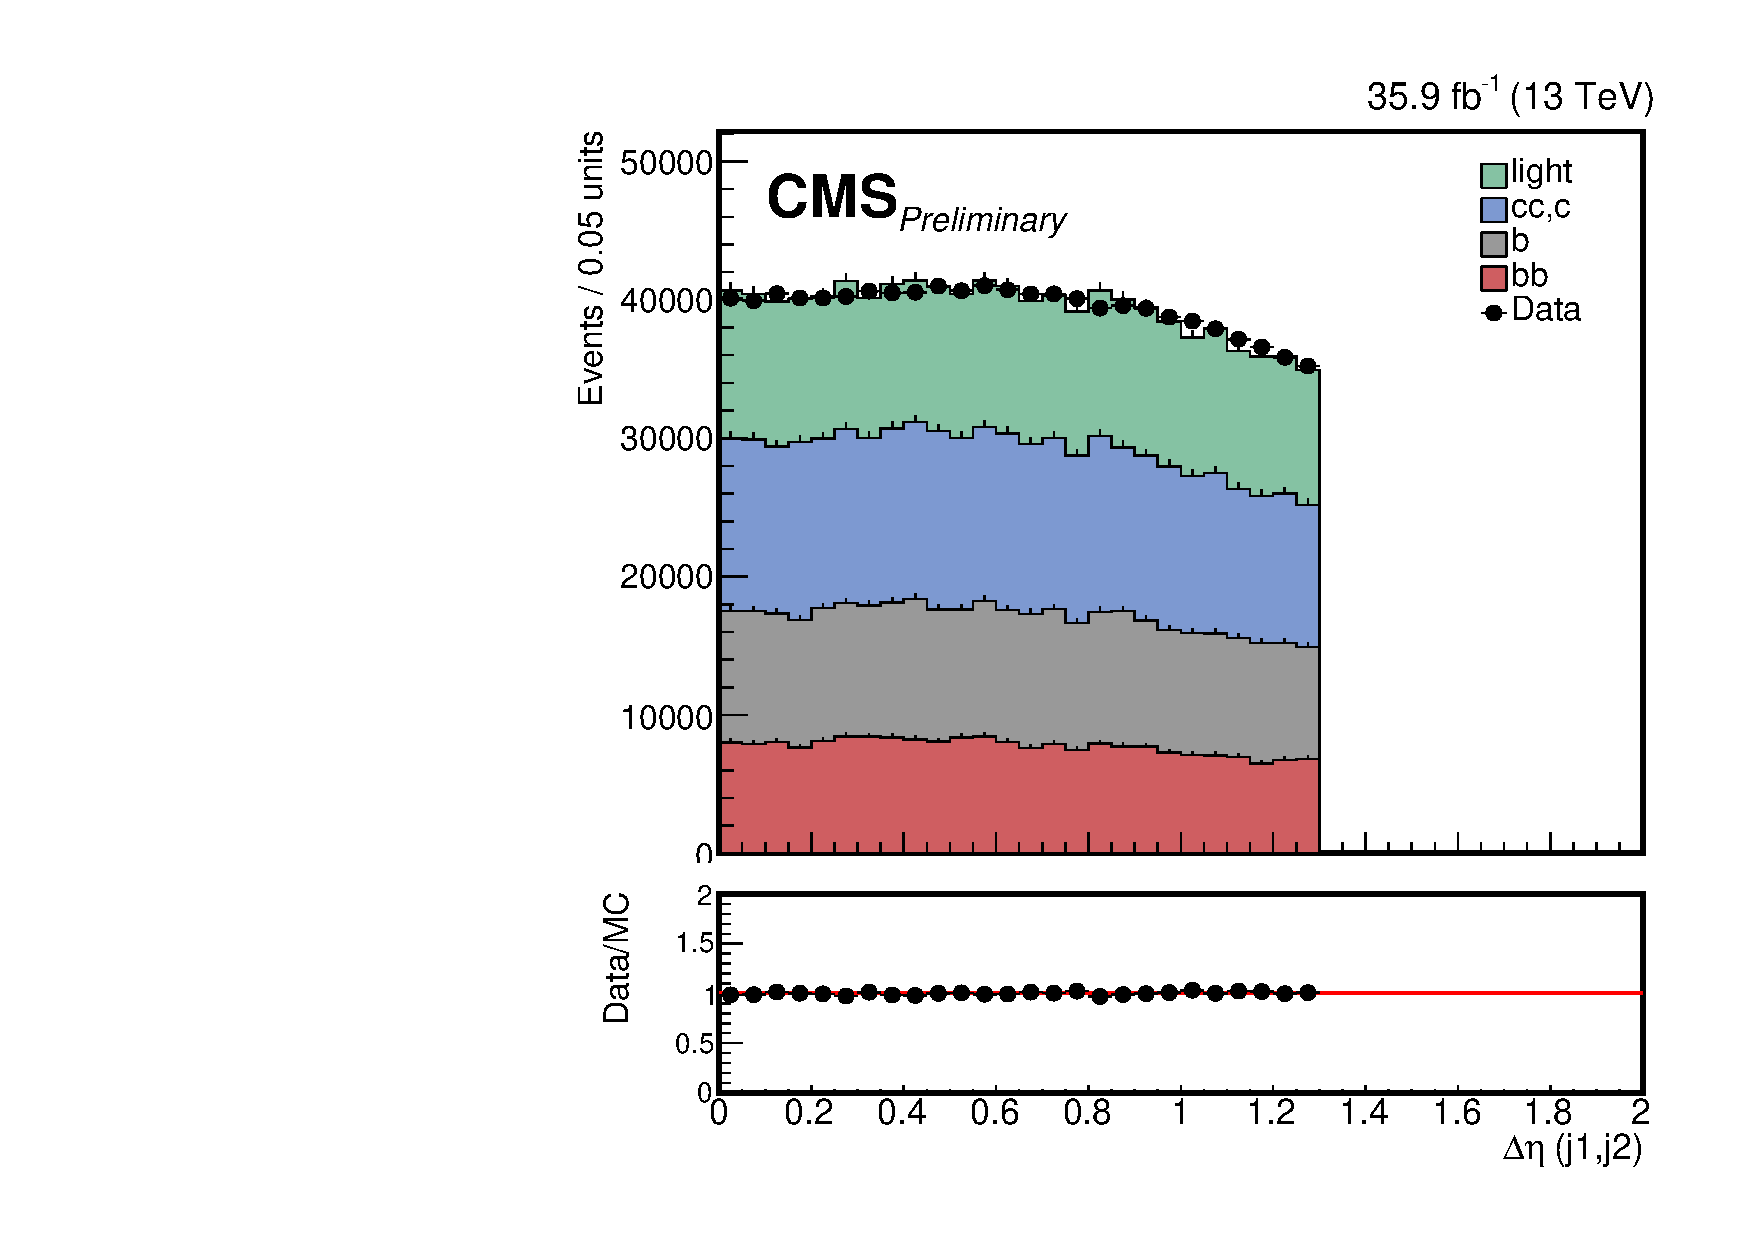
\includegraphics[width=0.5\textwidth]{Figures/dataMC_trig_antiDBT/deltaEta.pdf} \\
  \end{tabular}
  \caption{The comparison of data and background in inverse double-b region. Multi-jet events are seperated into four categories summarized in the table 3.10. From top to buttom are the comparison of PUPPI soft-drop mass, $\tau _{21}$ of leading (left) and next leading (right) AK8 jet, the reduced mass (buttom left), and |$\Delta \eta $ (the two leading AK8 jets)| (buttom right).}
  \label{fig:hvt_brs}
\end{figure}

\begin{figure}[t]
  \centering
  \begin{tabular}{cc}
    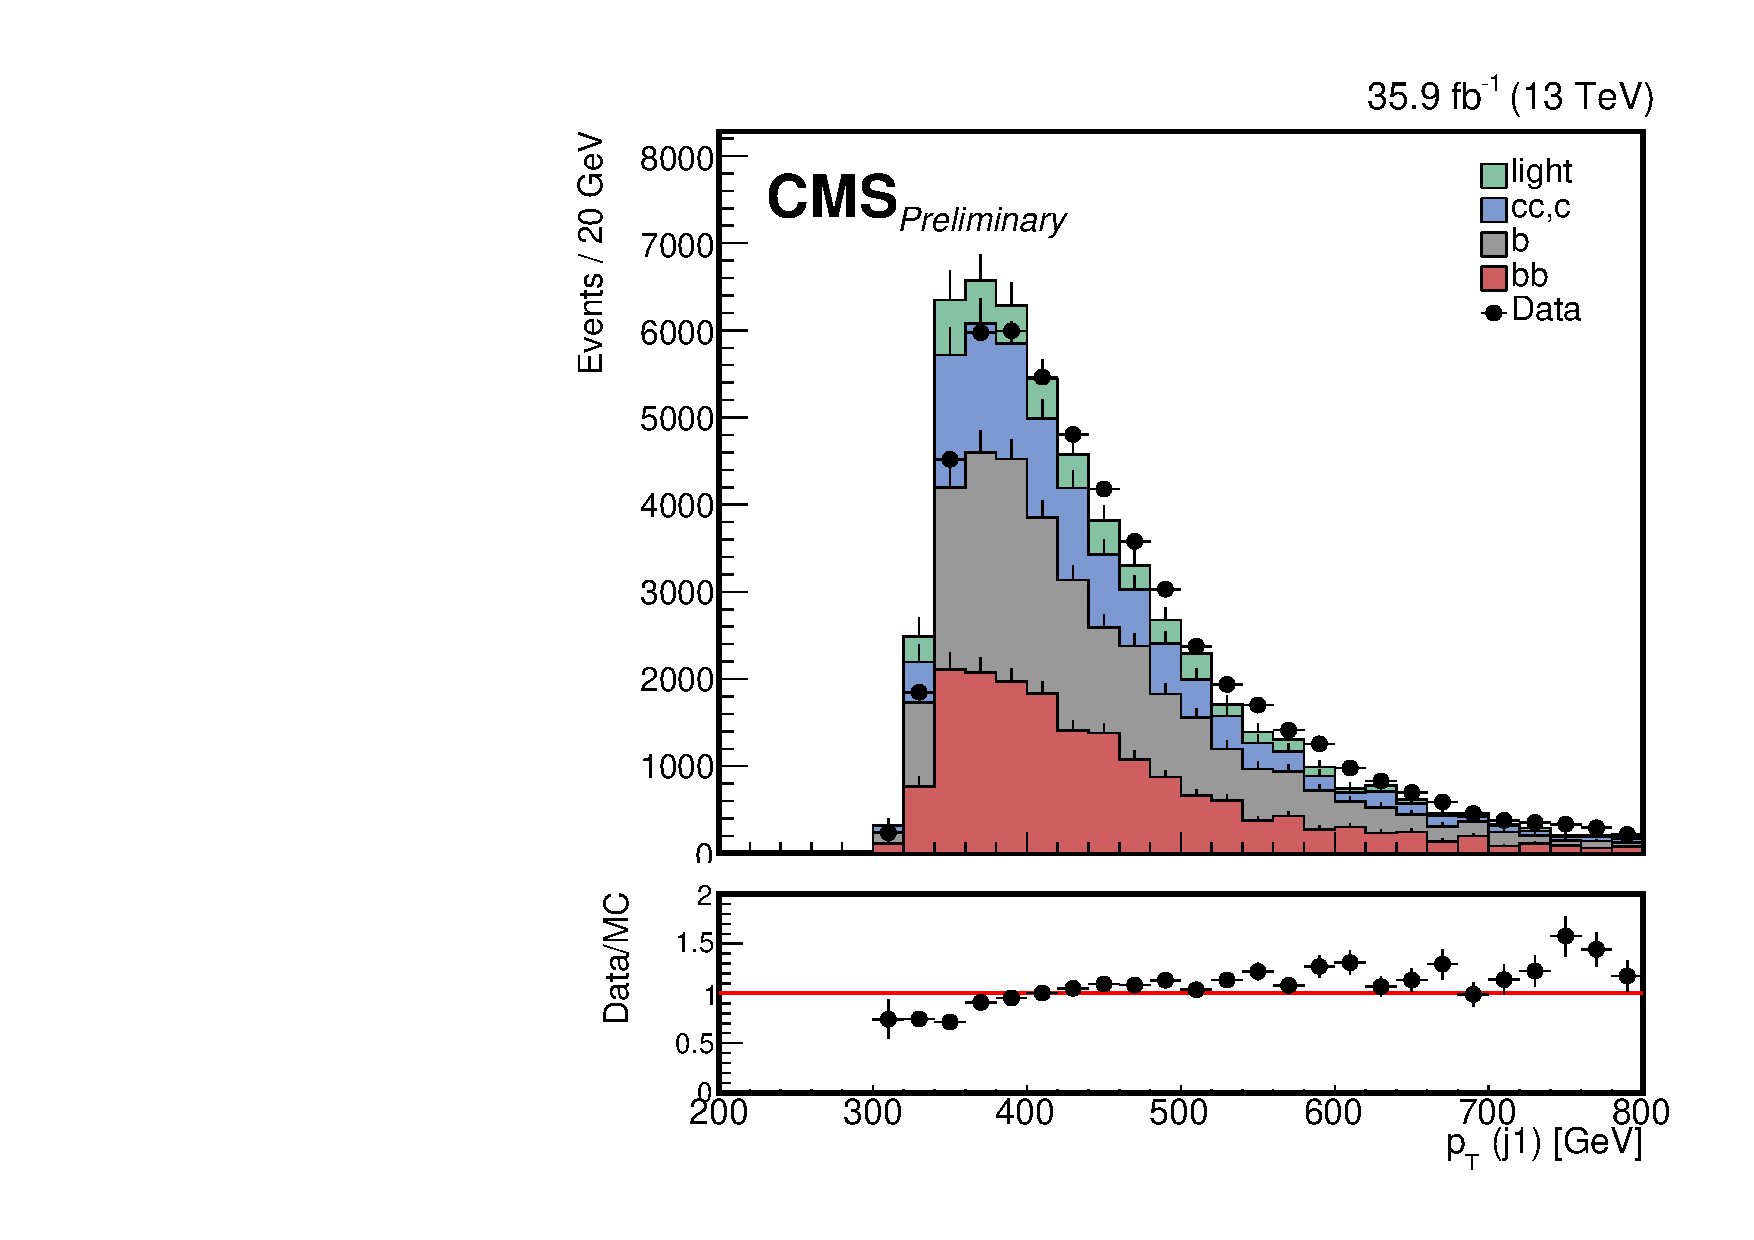
\includegraphics[width=0.5\textwidth]{Figures/dataMC_trig_antiTau21/pt_j0.pdf} &
    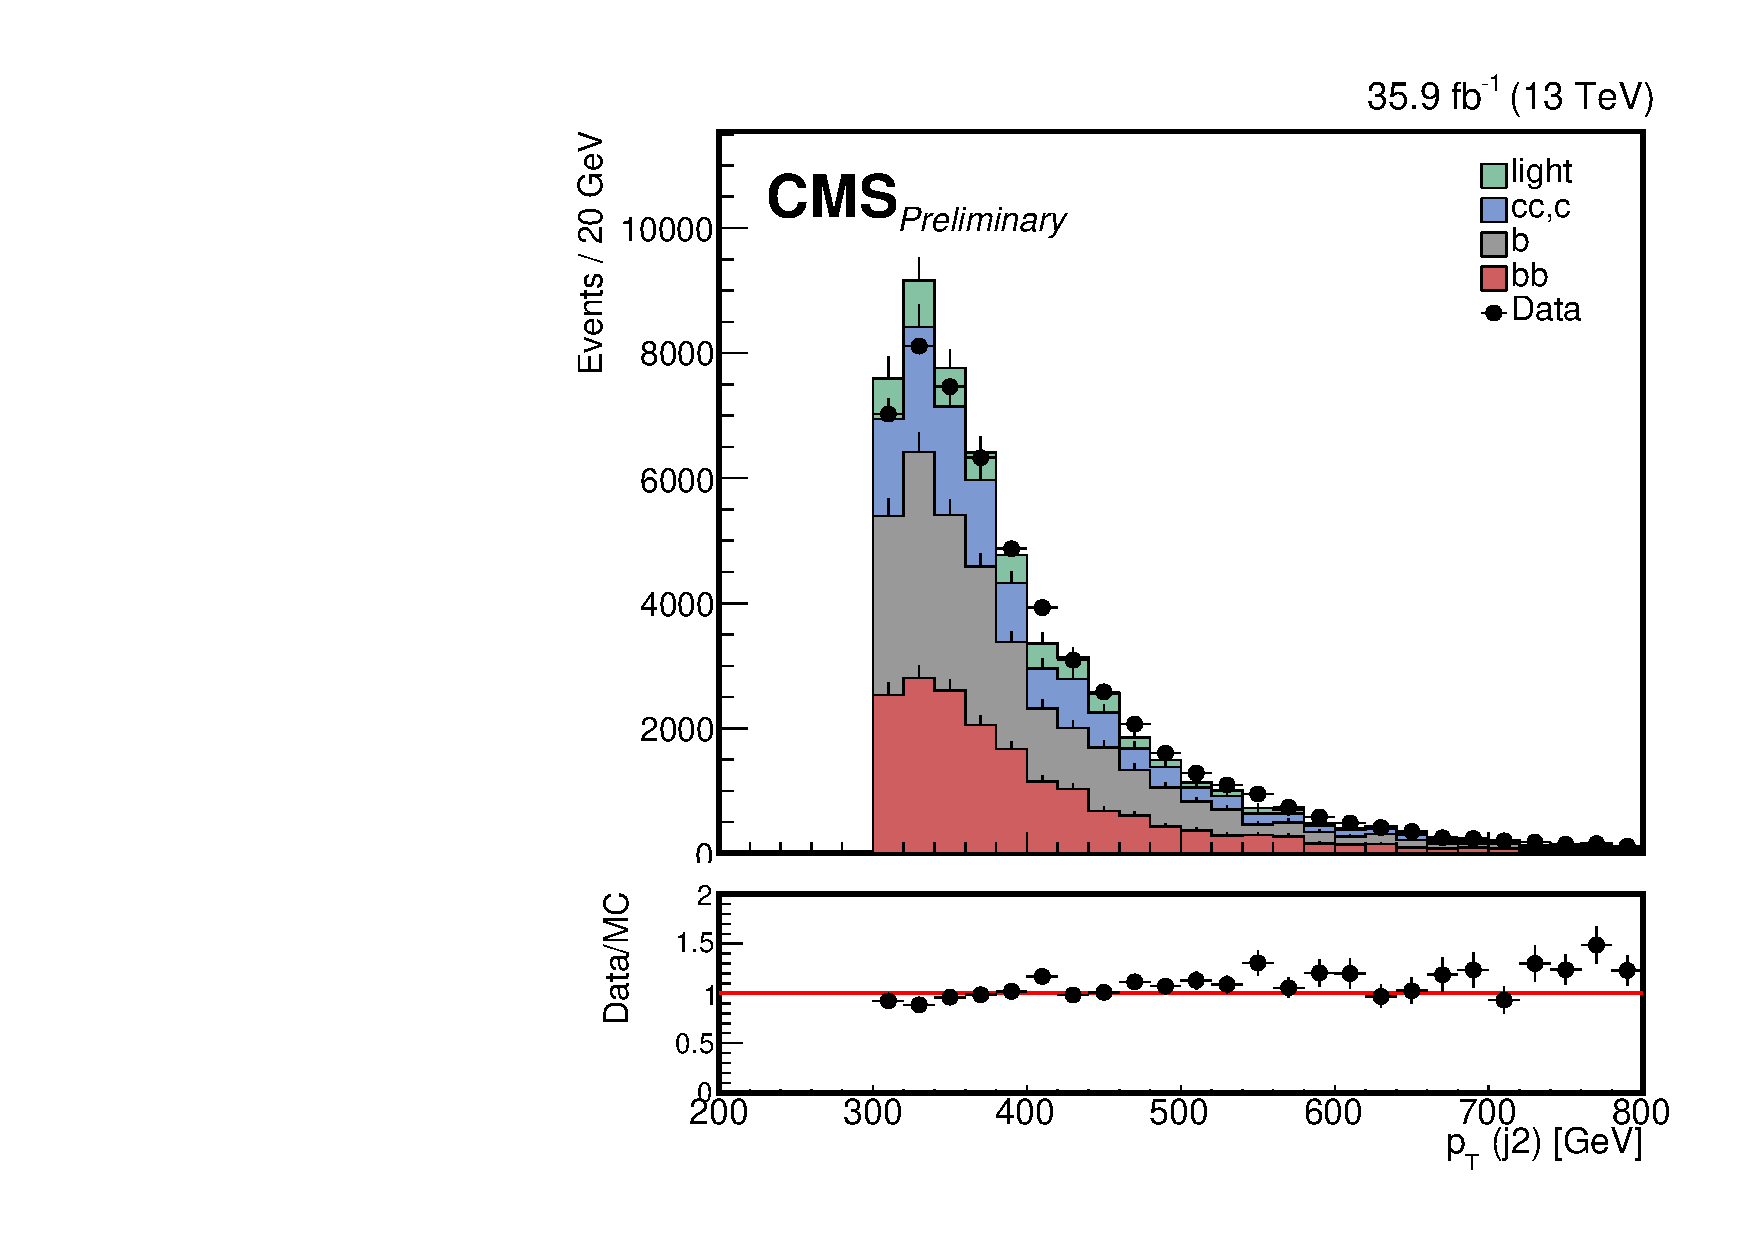
\includegraphics[width=0.5\textwidth]{Figures/dataMC_trig_antiTau21/pt_j1.pdf} \\
     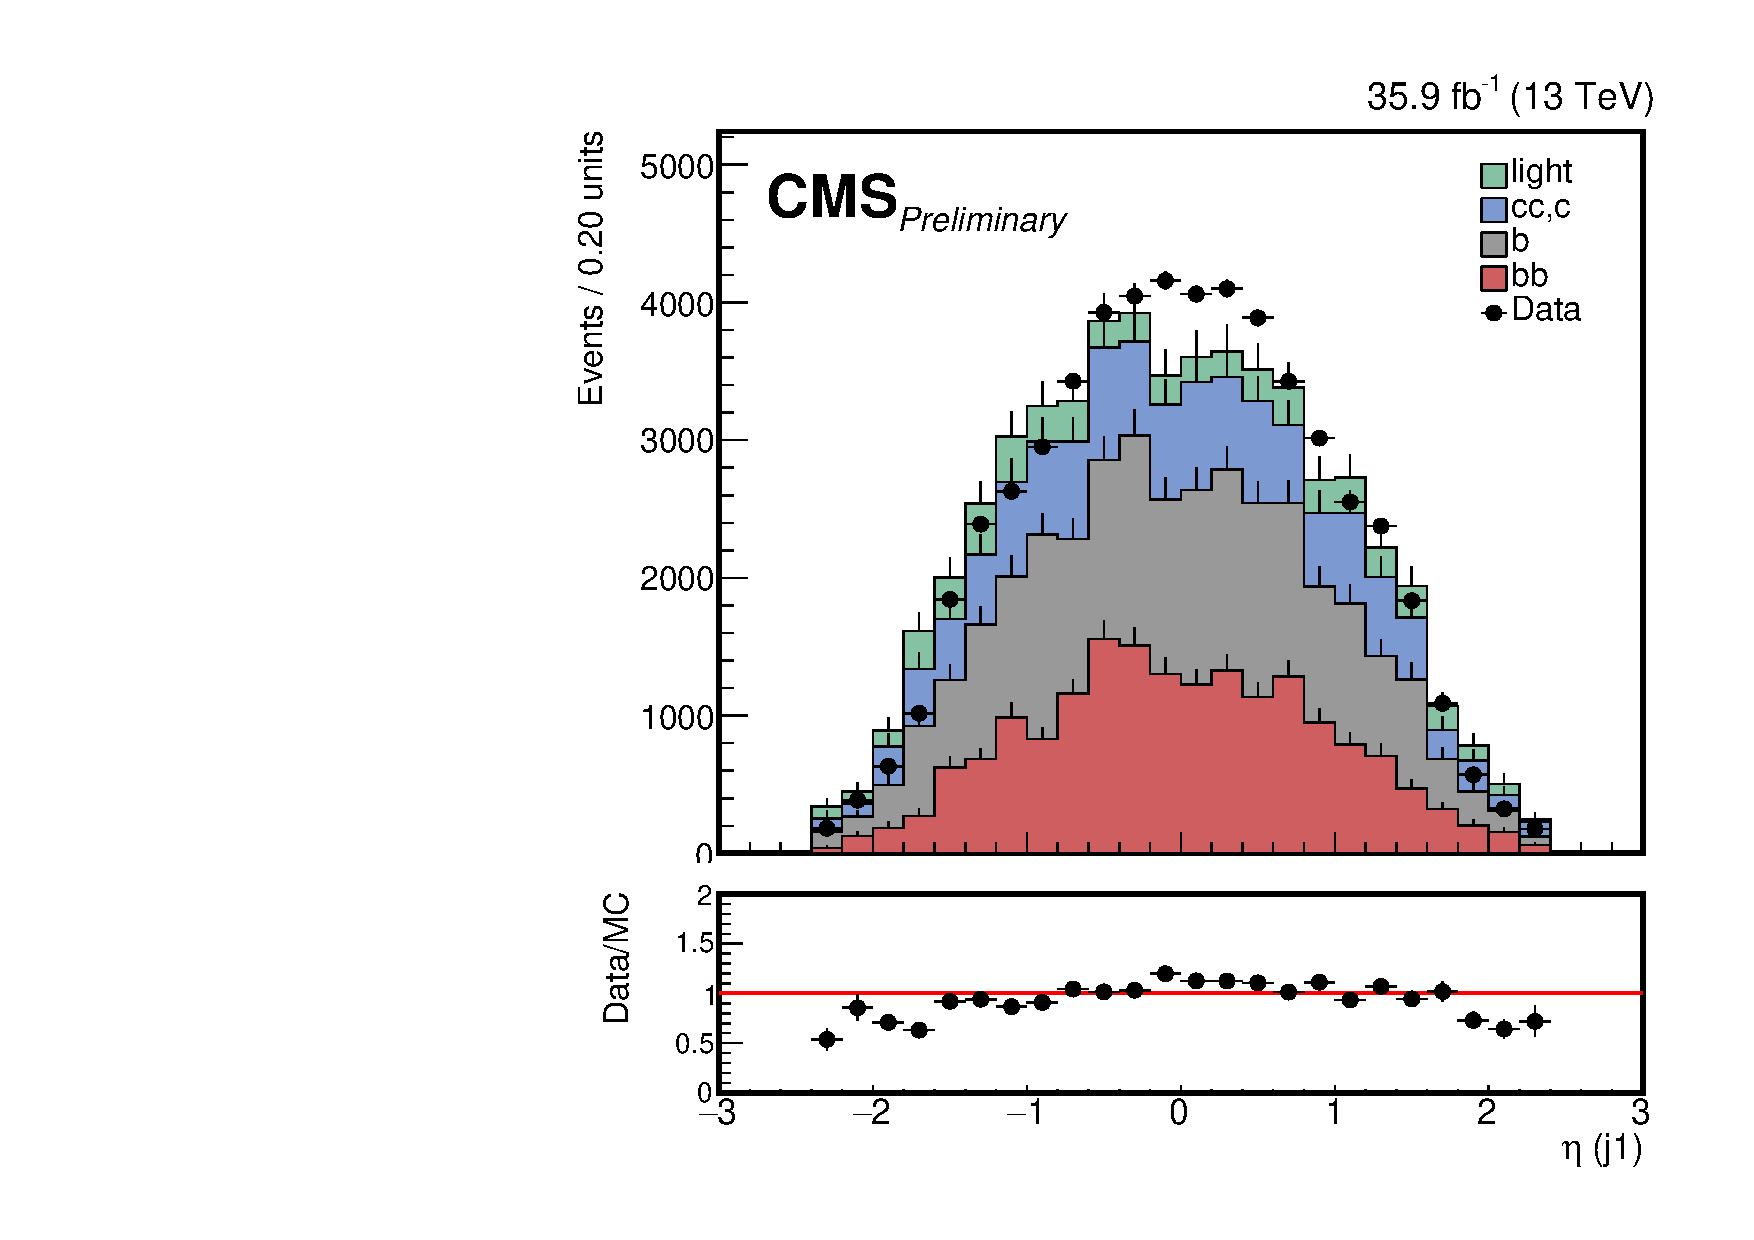
\includegraphics[width=0.5\textwidth]{Figures/dataMC_trig_antiTau21/eta_j0.pdf} &
    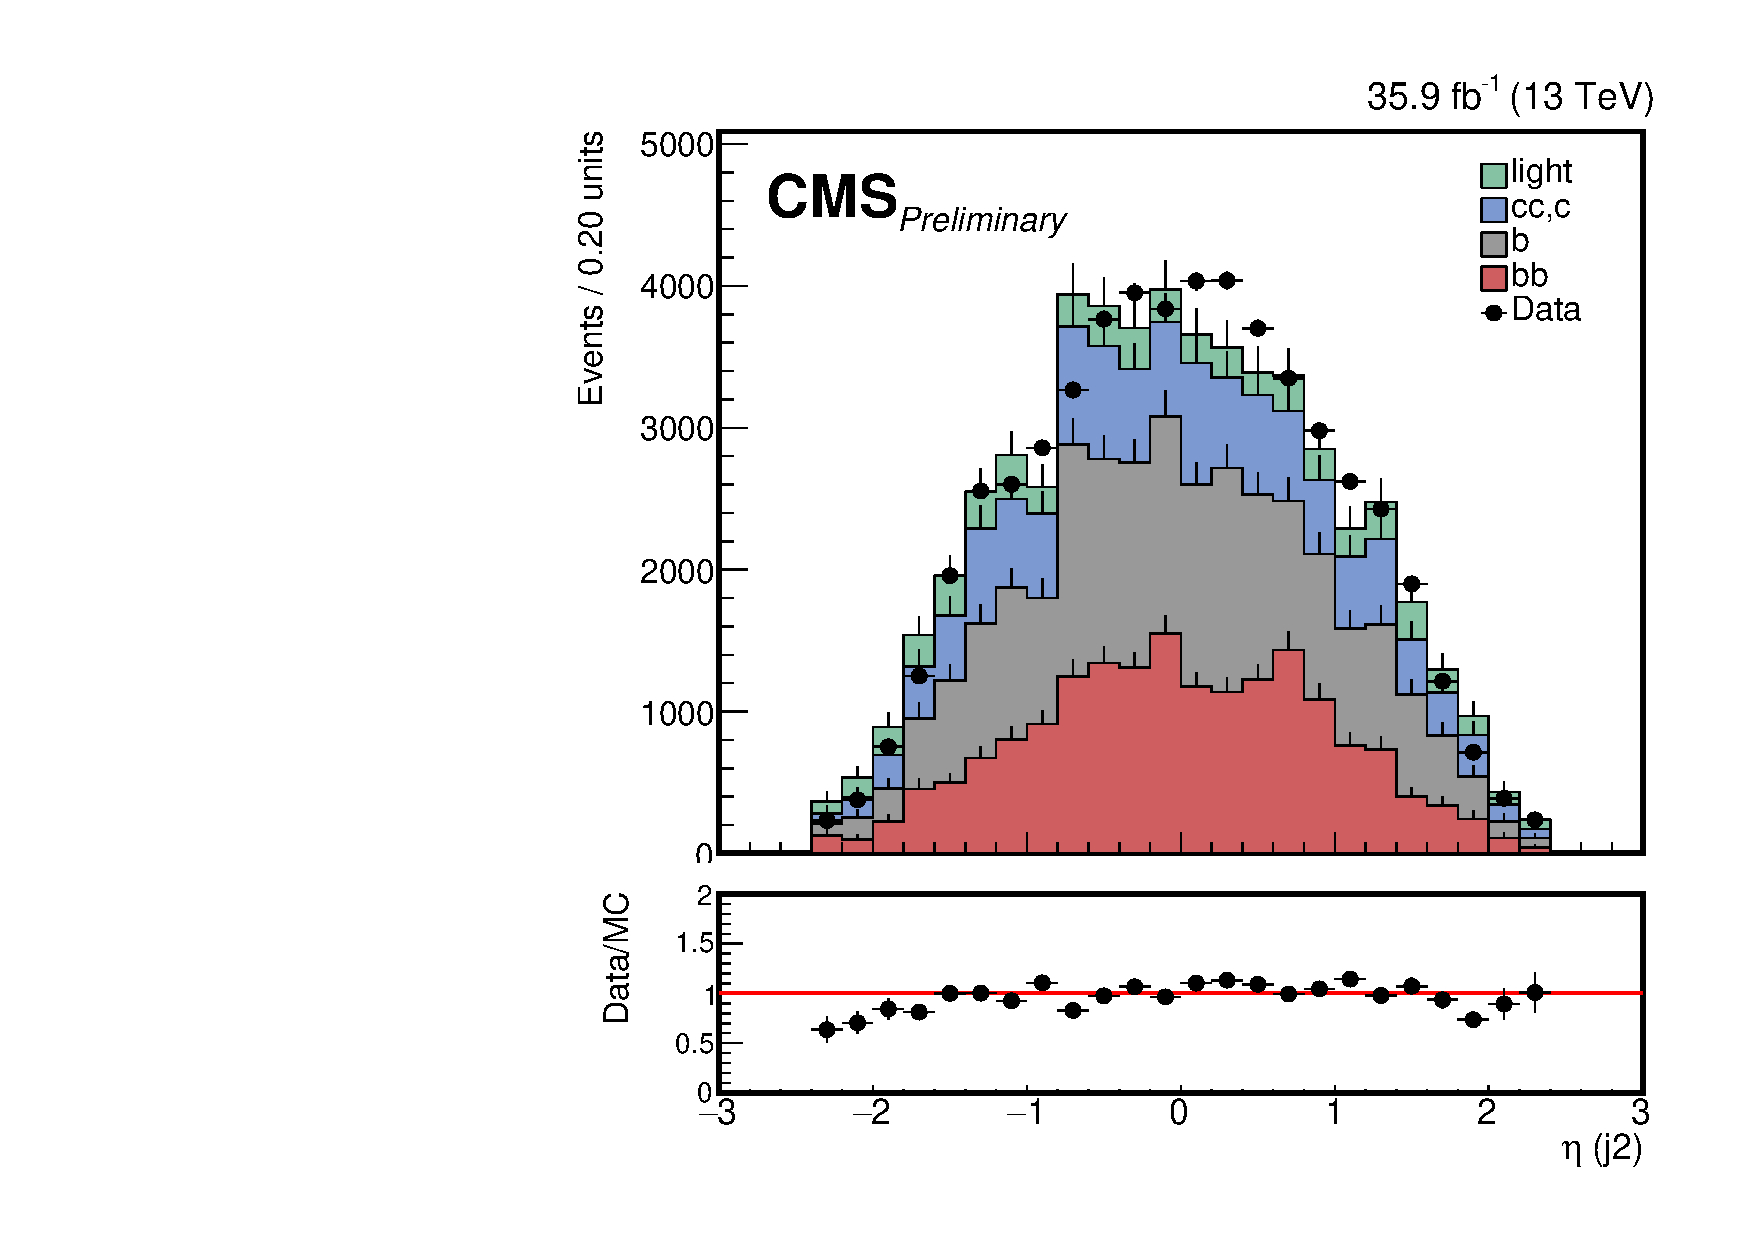
\includegraphics[width=0.5\textwidth]{Figures/dataMC_trig_antiTau21/eta_j1.pdf} \\
     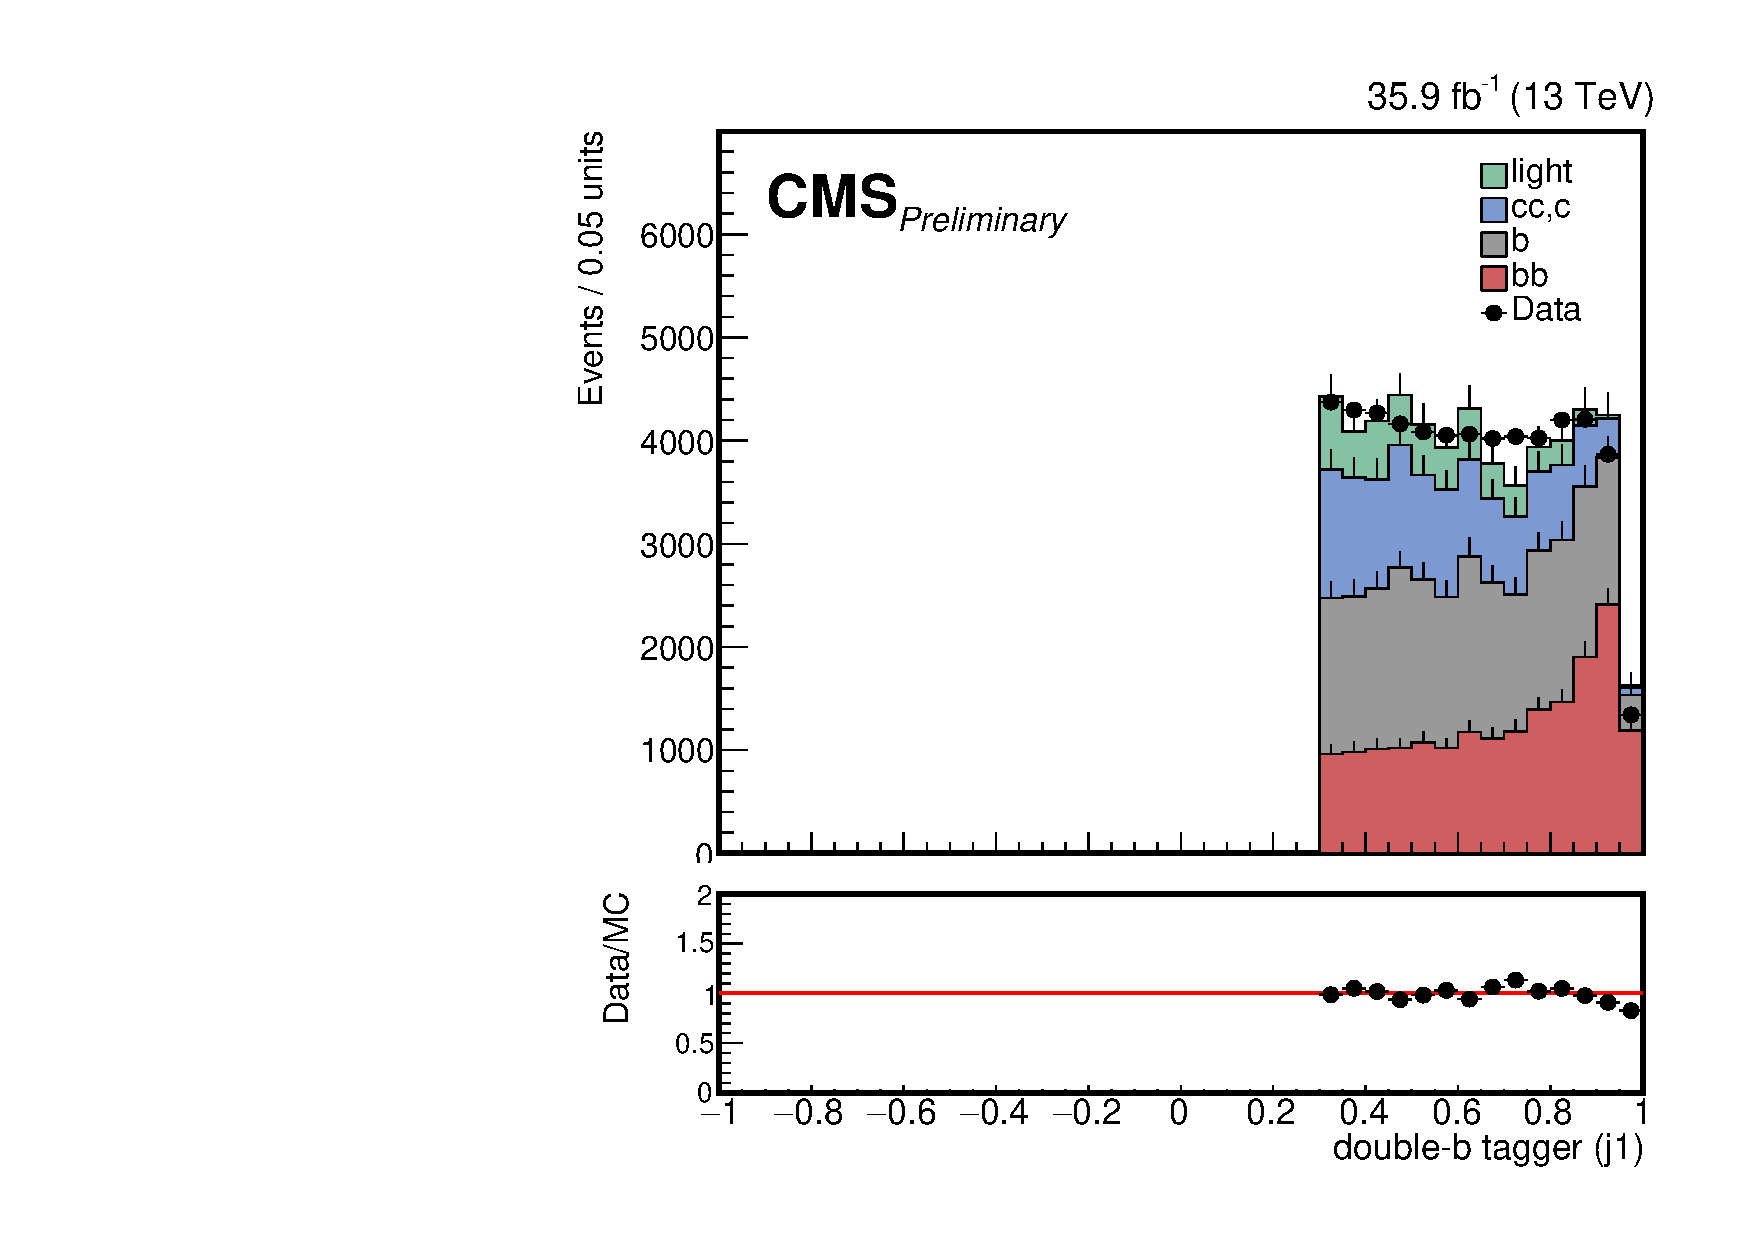
\includegraphics[width=0.5\textwidth]{Figures/dataMC_trig_antiTau21/doubleSV_j0.pdf} &
    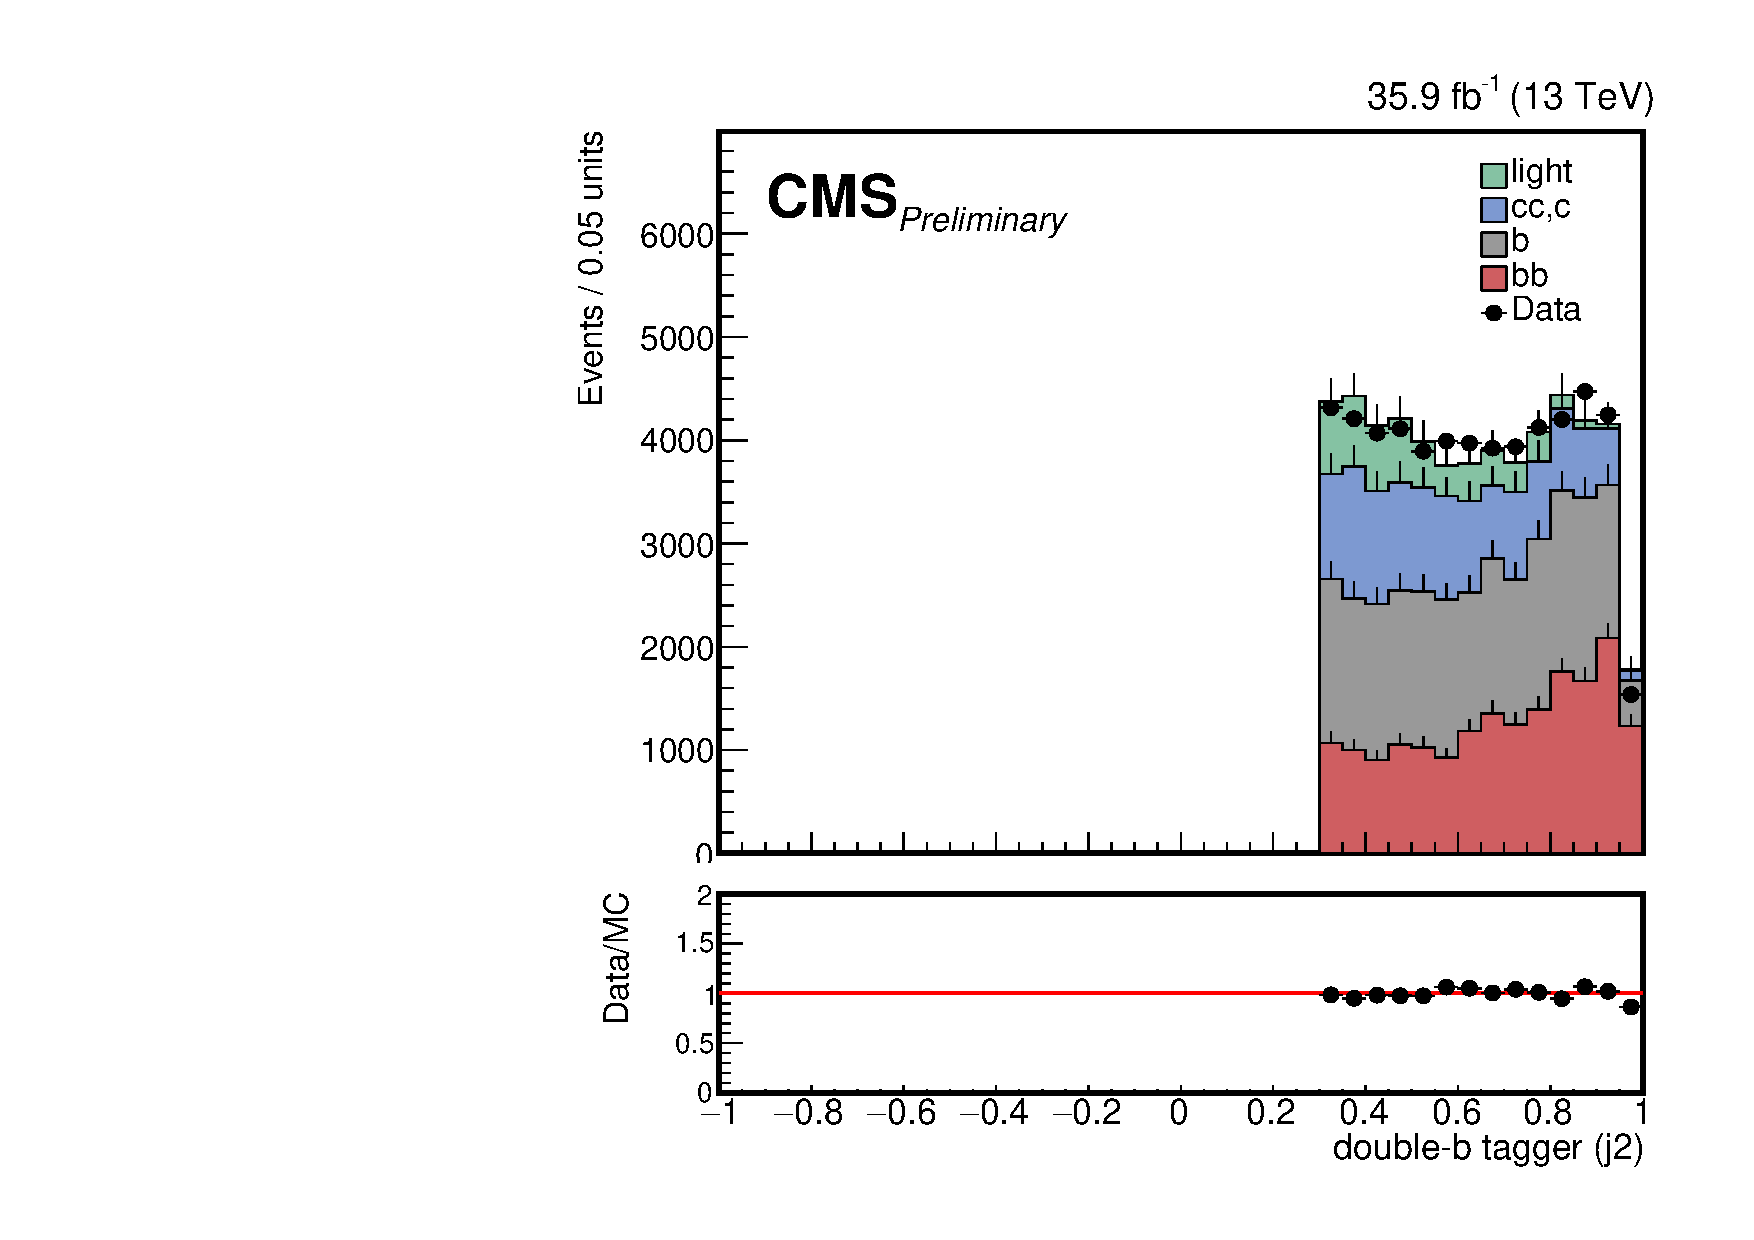
\includegraphics[width=0.5\textwidth]{Figures/dataMC_trig_antiTau21/doubleSV_j1.pdf} \\
  \end{tabular}
  \caption{The comparison of data and background in inverse $\tau _{21}$ region. Multi-jet events are seperated into four categories summarized in the table 3.10. From top to buttom are the comparison of $p_{T}$, $\eta $, and double-b tagger of leading (left) and next leading (right) AK8 jet.}
  \label{fig:hvt_brs}
\end{figure}
\begin{figure}[t]
  \centering
  \begin{tabular}{cc}
    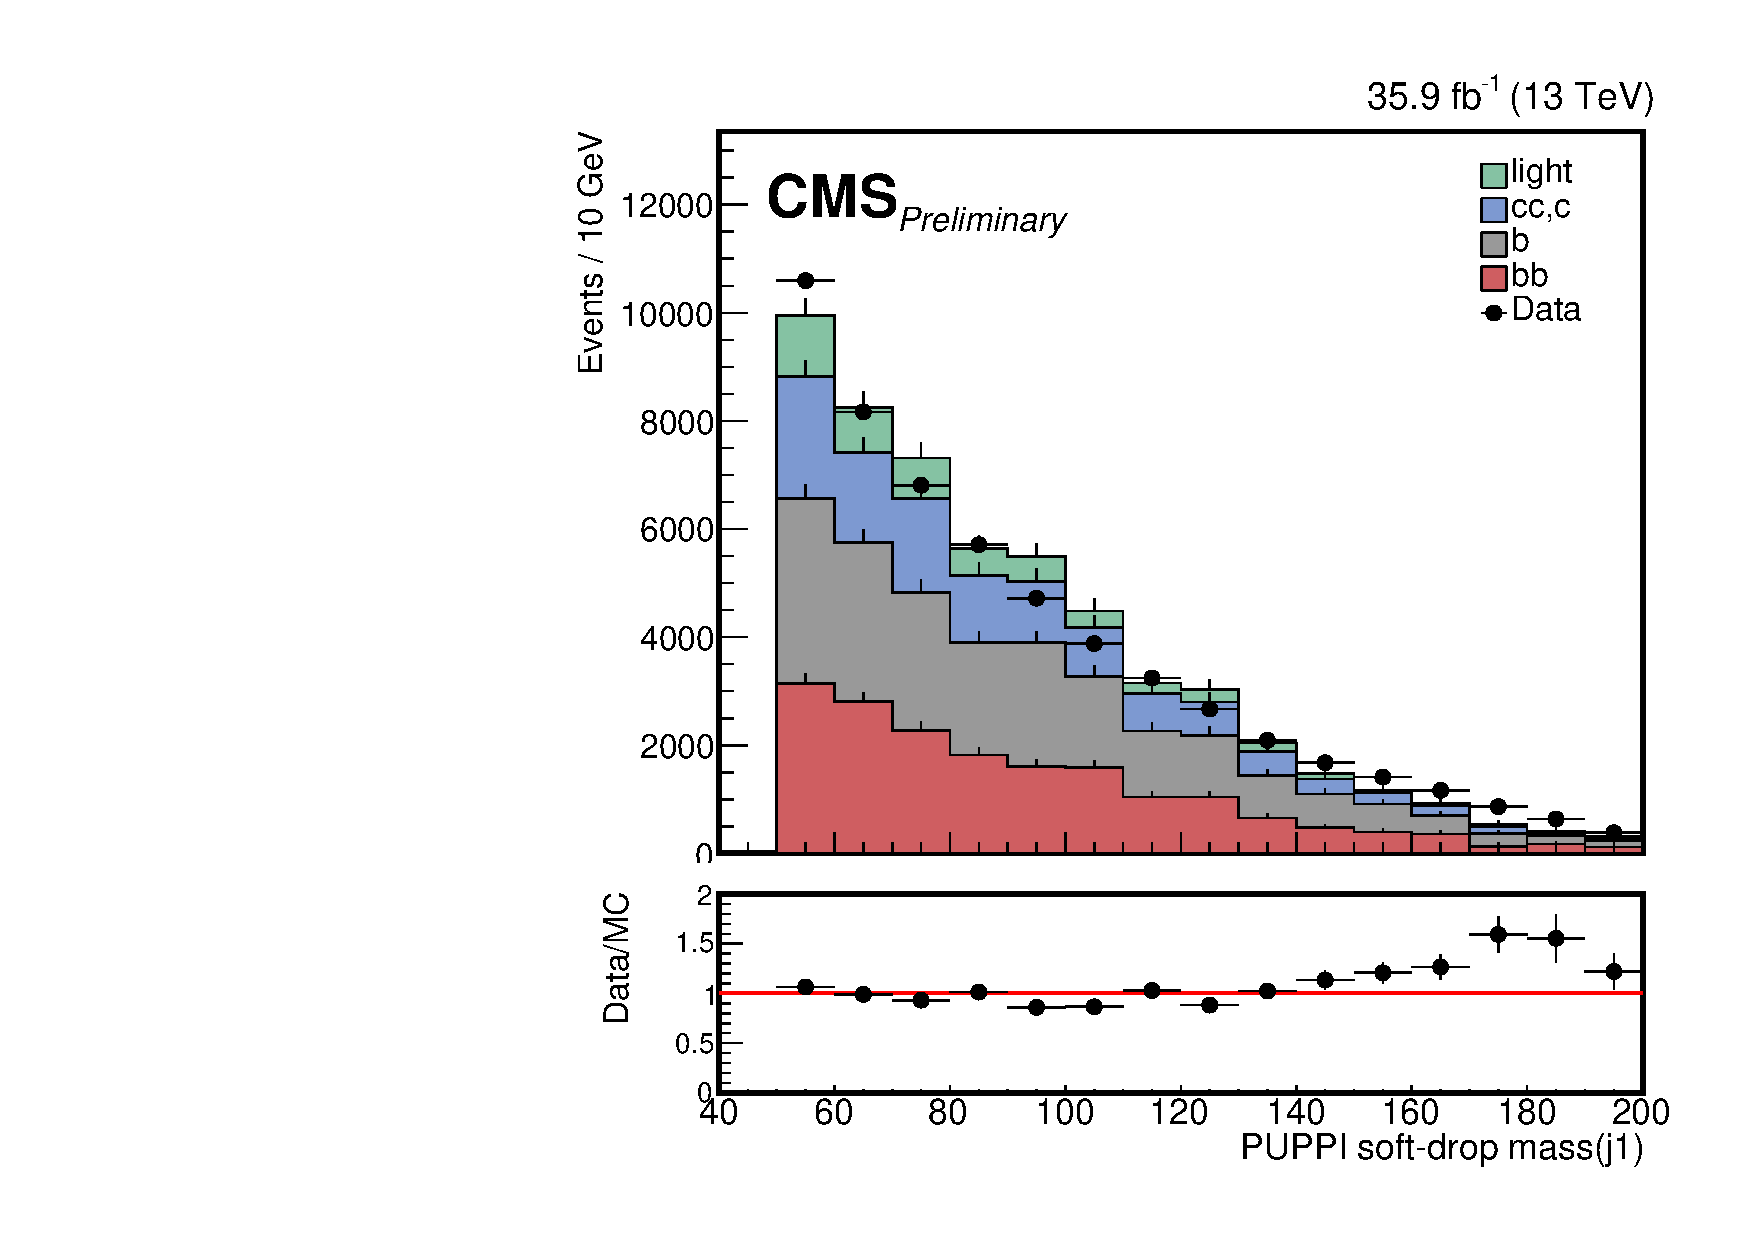
\includegraphics[width=0.5\textwidth]{Figures/dataMC_trig_antiTau21/puppiSDMassThea_j0.pdf} &
    \includegraphics[width=0.5\textwidth]{Figures/dataMC_trig_antiTau21/puppiSDMassThea_j1.pdf} \\
     \includegraphics[width=0.5\textwidth]{Figures/dataMC_trig_antiTau21/puppiTau21_j0.pdf} &
    \includegraphics[width=0.5\textwidth]{Figures/dataMC_trig_antiTau21/puppiTau21_j1.pdf} \\
     \includegraphics[width=0.5\textwidth]{Figures/dataMC_trig_antiTau21/totalMassRed.pdf} &
    \includegraphics[width=0.5\textwidth]{Figures/dataMC_trig_antiTau21/deltaEta.pdf} \\
  \end{tabular}
  \caption{The comparison of data and background in inverse $\tau _{21}$ region. Multi-jet events are seperated into four categories summarized in the table 3.10. From top to buttom are the comparison of PUPPI soft-drop mass, $\tau _{21}$ of leading (left) and next leading (right) AK8 jet, the reduced mass (buttom left), and |$\Delta \eta $ (the two leading AK8 jets)| (buttom right).}
  \label{fig:hvt_brs}
\end{figure}
%For each distribution, all selection described in previous section is required except the variable itself and double-b tagger discriminant.  
		% Chapter Backgrpund

\chapter{Background Estimation} \label{Background}
In this channel whose final state are four b-flavor jets, main background contribution comes from multi-jet events.
The background estimation in the study combines two method used in 2015 research: alphabet and bump hunt into alphabet assisted bump hunt.
 

\section{Bump Hunt}
The concept of searches for heavy resonance can be seen directly as finding a bump on the top of the smooth background, which is shown in figure 4.1. The fitted target is the mass spectrum of heavy resonances. The prababilty density function used in fitting are level-exponential function for data and Gaussian for signal.
\begin{figure}[t]
  \centering
  \begin{tabular}{c}
    \includegraphics[width=0.5\textwidth]{Figures/cart.pdf} 
   
  \end{tabular}
  \caption{The cartoon of a bump on the background.}
  \label{fig:hvt_brs}
\end{figure}

\section{Alphabet}
Alphabet method evoled from ABCD method which assumes the background is homogenously distributed on the two-dimension histogram. The histogram is sepearted into signal region and sideband region. The background in signal region can be extrapolated from sideband region. For example, if we see the figure 4.2, the number of events in signal region can get by:
\begin{equation} \label{eq1}
\centering
\begin{split}
\frac{N_{signal}}{N_{anti-tag}} = \frac{N_{side band B}}{N_{side band A}} = \frac{N_{side band D}}{N_{side band C}}, \\
N_{signal} = \frac{N_{side band B} \times N_{anti-tag}}{N_{side band A}} = \frac{N_{side band D} \times N_{anti-tag}}{N_{side band C}} \\
= N_{anti-tag} \times R_{p/f}, \\
\end{split}
\end{equation}
where N is the number of events located in the square region. The ratio $\frac{N_{signal}}{N_{anti-tag}}$ is referred as $R_{p/f}$ in the section. If the $R_{p/f}$ has dependence on the mass of the leading AK8 jet, one should use Alphabet method instead of ABCD method, as figure 4.3 and 4.4 show. Alphabet method gives $R_{p/f}$ a dependence on the mass of the leading AK8 jet:
\begin{equation} \label{eq2}
\begin{split}
N_{signal} = N_{anti-tag} \times R_{p/f} (M_{leading AK8}).
\end{split}
\end{equation}
The $R_{p/f}$ is derived in each bin of the mass of leading AK8 jet in mass side band. All $R_{p/f}$ of each bin is fitted together by a quadratic polynominal fit to interpolate the $R_{p/f}$ in the region of mass of signal. The fit results are shown in figure 4.4. Finally, the predicted background is get from an anti-tagged event weighted according to the mass of its leading AK8 jet. Figure 4.5 is predicted background in both LL and TT region. 

\begin{figure}[t]
  \centering
  \begin{tabular}{c}
    \includegraphics[width=0.5\textwidth]{Figures/cart2.pdf} 
 
  \end{tabular}
  \caption{The cartoon of a two dimensional distribution.}
  \begin{tabular}{cc}
    \includegraphics[width=0.5\textwidth]{Figures/al/2d_TT.pdf} &
   \includegraphics[width=0.5\textwidth]{Figures/al/2d_LL.pdf} 
  \end{tabular}
  \caption{The double-d tagger versus the mass of the leading AK8 jet distribution in TT (left) and LL (right) region.}
\end{figure}



\begin{figure}[t]
  \centering
 \begin{tabular}{cc}
    \includegraphics[width=0.5\textwidth]{Figures/al/1d_TT.pdf} &
   \includegraphics[width=0.5\textwidth]{Figures/al/1d_LL.pdf} 
   
  \end{tabular}
  \caption{The $R_{p/f}$ and its quadratic fit in TT (left) and LL (right) region.}
  \label{fig:hvt_brs}
\end{figure}

\begin{figure}[t]
  \centering
 \begin{tabular}{cc}
    \includegraphics[width=0.5\textwidth]{Figures/al/mjj_TT.pdf} &
   \includegraphics[width=0.5\textwidth]{Figures/al/mjj_LL.pdf} 
   
  \end{tabular}
  \caption{The $R_{p/f}$ and its quadratic fit in TT (left) and LL (right) region.}
  \label{fig:hvt_brs}
\end{figure}

\clearpage
\section{Alphabet Assisted Bump Hunt}
The two background estimation methods, alphabet and bump hunt, use orthogonal information from data.
While bump hunt drive in signal region, alphabet extrapolate from data in side band region. 
Therefore, we can combine two method into alphabet assisted bump hunt.

The estimation is inplemented as follow:
\begin{itemize}
\item Define a tagging and anti-tagging region. The double-b tagger working point is used as a discriminator here.
\item Derive the ratio of number of events in tagging region to that of anti-tagging region, which referred below $" R_{p/f} "$.
\item The dependence of $R_{p/f}$ on $M_{jj}$ and that on $M_{Higgs Jet}$ are considered, while the latter is small enough to be ignored. The shape and the numbner of estimated background can be get from:
\begin{equation} \label{eq3}
\begin{split}
Bkg(M_{jj})= R_{p/f}(M_{jj}) \times Anti-tag(M_{jj}), 
\end{split}
\end{equation}
which can be further reduced to 
\begin{equation} \label{eq4}
\begin{split}
R_{p/f}(M_{jj})= 1+(M_{jj} \times lin_{par}) \\
Bkg(M_{jj})= (1+(M_{jj} \times lin_{par})) \times Anti-tag(M_{jj}),
\end{split}
\end{equation}
where the parameters in Bkg($M_{jj}$) are initialized the same as Anti-tag($M_{jj}$), and $lin_{par}$ is a parameter of the linear dependence on $M_{jj}$. The initialized p.d.f is referred as pre-fit.
\item  The function Bkg($M_{jj}$) fits on the data in signal region to finish a post-fit procedure. 

\end{itemize}
\end{linenumbers}

%----------------------------------------------------------------------------------------
%	BIBLIOGRAPHY
%----------------------------------------------------------------------------------------

{\setstretch{1.15} \sloppy \printbibliography[heading=bibintoc]}

%----------------------------------------------------------------------------------------

\end{document}  
